%%%%%%%%%%%%%%%%%%%%%%%%%%%%%%%%%%%%%%%%%%%%%%%%%%%%%%%%%%%%% 
% Preamble Options
%%%%%%%%%%%%%%%%%%%%%%%%%%%%%%%%%%%%%%%%%%%%%%%%%%%%%%%%%%%%%

% Select build mode from:
%     quick - try to compile quickly (no extras, remove front pages)
%     debug - add grid lines/compile times (print variables)
%     proof - local version of "final" 
%     final - Final publishable version (calls PurdueThesis - requires LuaLaTeX)
\def\ZZbuildmode{final}

% Input arguments required by PurdueThesis

% ----------------- Author/Document Info -----------------
% Auuthor Name
\def\ZZauthor{Jonathan Richmond}

% "May XXXX", "August XXXX", or "December XXXX"
\def\ZZgraduation{May 2024}

% Title
\def\ZZtitle{WORKING TITLE: Utilizing Invariant Manifolds of Cislunar Periodic Orbits for Efficient Deep Space Tansfers}


% -------------------- Degree Program ---------------------
% Either:
%     Doctor of Philosophy
%     Master of Science in Aeronautics and Astronautics
\def\ZZdegree{Master of Science in Aeronautics and Astronautics}

% Either "A Dissertation" or "A Thesis"
\def\ZZdocument{A Thesis}


% --------------- Final Draft Defaults (AAE) ---------------

% Purdue AAE (West Lafayette)
\def\ZZinstitution{Purdue University}
\def\ZZcampus{West\space Lafayette}
\def\ZZprogram{Aeronautics and Astronautics}

% Defaults for final draft
%      These are overwritten in PurdueThesisNL.cls but 
%      not in PurdueThesis.cls 
\def\ZZshowgridlines{false}
\def\ZZshowmarginlines{false}
\def\ZZshowtimestamp{false}
\def\ZZtodonotes{false}
\def\ZZatinformation{}
\def\ZZshowcolophon{false}
\def\ZZshowdiagonalline{false}

% Build the document this will select the document class based on :
%    quick/debug/proof - Local simplified PurdueThesis.cls file
%                final - Official PurdueThesis.cls file
\RequirePackage{ifthen}
\ifthenelse{\equal{\ZZbuildmode}{final}}
{\documentclass{PurdueThesis}}{\documentclass{PurdueThesisNL}}

% Set up the latex document w/ imports, definitions, and 
% template customizations
\ConfigureBibliography
% \graphicspath{{eps/}{tiff/}}
\graphicspath{{figures/}{figures/template}}

% Look in the "packages" subfolder for packages.
% This is done to reduce the number of files in the main thesis folder
% so the ones in there are easier to find.
\makeatletter
  \def\input@path{{packages/}}
\makeatother

% The vertical space between a table heading and the table contents in a tabular environment.
\newcommand{\tabularspace}{\noalign{\vspace*{2pt}}}

% Define boolean variables that contorl how the document is compiled
\newboolean{quick}
\newboolean{debug}
\newboolean{proof}
\newboolean{final}
\newboolean{quick-or-debug}
\newboolean{proof-or-final}

\ifthenelse{\equal{\ZZbuildmode}{quick}}
    {\setboolean{quick}{true}}{\setboolean{quick}{false}}
\ifthenelse{\equal{\ZZbuildmode}{debug}}
    {\setboolean{debug}{true}}{\setboolean{debug}{false}}
\ifthenelse{\equal{\ZZbuildmode}{proof}}
    {\setboolean{proof}{true}}{\setboolean{proof}{false}}
\ifthenelse{\equal{\ZZbuildmode}{final}}
    {\setboolean{final}{true}}{\setboolean{final}{false}}

\ifthenelse{\boolean{quick} \OR \boolean{debug}}
  {\setboolean{quick-or-debug}{true}}
  {\setboolean{quick-or-debug}{false}}
\ifthenelse{\boolean{proof} \OR \boolean{final}}
  {\setboolean{proof-or-final}{true}}
  {\setboolean{proof-or-final}{false}}

% -------------------- From Template -------------------

% So "_" will work in URLs when using BibTeX.
\usepackage[T1]{fontenc}

% The mathtools package
% (see http://mirror.utexas.edu/ctan/macros/latex/required/amsmath/amsmath.pdf)
% loads the amsmath package which defines the
%     align
%     align*
%     alignat
%     alignat*
%     equation
%     equation*
%     flalign
%     flalign*
%     gather
%     gather*
%     multitaper
%     multitaper*
%     split
% environments and extends amsmath by defining many other commands.
% See
%     https://ctan.org/pkg/amsmath
% for information about amsmath and
%     http://ctan.math.washington.edu/tex-archive/macros/latex/contrib/mathtools/mathtools.pdf
% for information about mathtools.
\usepackage{mathtools}

% Define \FigureDash.
% \FigureDash is a dash the width of a digit in the current font.
\usepackage{pa-figure-dash}

% For PurdueThesis, PuTh, TeX, LaTeX, METAFONT, METAPOST, etc. related logos.
\usepackage{pa-logos}

% (Or maybe use isomath instead?  -mark  2021-06-20)
% Follow ISO 80000-2:2019
%     o   put e, i, j, and pi in upright font automatically
%     o   use, for example, "\di x" to get "\,mathrm{d}\/x"
% This loads
%     o   amsmath.sty (which is already loaded above)
%     o   mathtools.sty
%     o   upgreek.sty
% Load the package.
\usepackage{pa-mismath}
    % Tell mismath to put e, i, j, and pi in upright font automatically.
    \enumber
    \inumber
    \jnumber
    \pinumber
  % To typeset math italic e, i, j, and pi use
  %     \mathit e
  %     \mathit i
  %     \mathit j
  %     \itpi


% Define \FloatBarrier
\usepackage{placeins}

% For highlighting text using \hl
\usepackage{soul}

% For \sfrac, used to do slanted fractions, similar to, e.g., 1/2, but 1 is small and high and 2 is small and low.
\usepackage{xfrac}

% For typographical conventions stuff including
%     \Emph{...}
%     \First{...}
%     \Keys{...}
%     \Literal{...}
%     \Menu{...}
%     \Place{...}
%     \Shell{...}
% This must be after
%     \usepackage{tikz}
\usepackage{pa-typographic-conventions}


% ----------------- Added Dependencies -----------------

% Generate lorem ipsum 
%    e.g.: \lipsum[1-2]
\usepackage{lipsum}

% To sort variables alphabetically in debug mode
\usepackage{datatool}

% Extra math symbols
%     mathbb
\usepackage{amssymb}

% Acronyms
\usepackage[acronym]{glossaries}
  \glsdisablehyper

% cleveref
%   For easier cross-referencing
%   Redefine the subref formatting so that you get:
%     Figure 1.1(a) instead of Figure 1.1a
\usepackage[noabbrev, capitalise]{cleveref}
  \captionsetup[subfigure]{subrefformat=simple,labelformat=simple}
  \renewcommand\thesubfigure{(\alph{subfigure})}

% Put table captions on top / adjust the spacing
\captionsetup[table]{
    position=above,
    belowskip=4pt
  }

% My packages (JHR)
\usepackage{float}



% Define \NL (newline) so LaTeX goes to the next output line.
% Just doing \\ complains
%     ! LaTeX Error: There's no line here to end.
% \mbox{} is an empty math box.
\newcommand{\NL}{\mbox{}\\}



% To keep track of variables used in the document
%    for optional printing when in debug mode
\makeatletter
    \newcommand*\paperVariables{}
    \newcommand*\paperSortVars{}
    \newcommand*\storeVariables[2]
    {\ifx\paperVariables\empty
        \def\paperVariables{{#1,#2}}%
    \else
        \g@addto@macro\paperVariables{, {#1,#2}}%
    \fi
    }
    \makeatother
    

% Use \varDef instead of \newCommand to track variables for debug mode
%       #1: latex command for the variable (e.g. \myAngle)
%       #2: symbol to use (e.g. a, A, \alpha)
%       #3: (optional) font class (e.g. \mathbb )
\def\temp{ \NewDocumentCommand{\varDef}{m m o e{_^}} }

\ExplSyntaxOn
\temp{%
    \IfValueTF{#3}{ %
        \newcommand{#1}{{#3{#2}}\sb{\IfValueT{#4}{#4}}\sp{\IfValueT{#5}{#5}}}%
    }{%
        \newcommand{#1}{{#2}\sb{\IfValueT{#4}{#4}}\sp{\IfValueT{#5}{#5}}} %
    }%
    % \IfValueT{#5}{^{#5}}%
    % Only store variables if needed for debug mode
    \ifthenelse{\equal{debug}{\ZZbuildmode}} { %
        \storeVariables{#1}{#2}}{} %
} %
\ExplSyntaxOff


% Vector formatting
\newcommand{\vectorFmt}[1]{\pmb{#1}}
\newcommand{\unitVecFmt}[1]{\hat{#1}}
\newcommand{\sub}[2]{{#1}_{#2}}
\newcommand{\upRight}[2]{{#1}^{#2}}
\newcommand{\upLeft}[2]{{}^{#2} {#1}}
\newcommand{\firstDerivative}[1]{\dot{#1}}
\newcommand{\secondDerivative}[1]{\ddot{#1}}

% Define useful variables of the form:
%    \vardef{\command}{var-name}[\format] 

% Testing out some basic ones
\varDef{\zNd}{z}
\varDef{\xNd}{x}
\varDef{\yNd}{y}
\varDef{\xDim}{X}
\varDef{\yDim}{Y}
\varDef{\zDim}{Z}
\varDef{\angleTwo}{\beta}
\varDef{\angleOne}{\alpha}
\varDef{\angleFour}{\Pi}
\varDef{\angleThree}{\Gamma}
\varDef{\otherCvar}{C}
\varDef{\nBody}{N}

% Math
\varDef{\Real}{R}[\mathbb]
\varDef{\Complex}{C}[\mathbb]

% Stats
\varDef{\Normal}{N}[\mathcal]
\varDef{\Uniform}{U}[\mathcal]
\varDef{\ExpVal}{E}[\mathbb]

% Dynamical Systems
\varDef{\lagrangian}{L}[\mathcal]
\varDef{\hamiltonian}{H}[\mathcal]

% To show how formatting is handled
\varDef{\vectorFormat}{x}[\vectorFmt]
\varDef{\unitVectorFormat}{x}[\unitVecFmt]

% How about superscripts?
\varDef{\xSquared}{x}^{2}
\varDef{\xSubTwo}{x}_{2}
\varDef{\xSubTwoSquared}{x}_{2}^{2}
\varDef{\aVectorSquared}{y}[\vectorFmt]^{2}

% Rates (Mine)
\varDef{\rbardot}{\rbar}[\dot]
\varDef{\rbarddot}{\rbar}[\ddot]
\varDef{\rdot}{r}[\dot]
\varDef{\rhobardot}{\rhobar}[\dot]
\varDef{\rhodot}{\rho}[\dot]
\varDef{\thetadot}{\theta}[\dot]
\varDef{\Xddot}{X}[\ddot]
\varDef{\xddot}{x}[\ddot]
\varDef{\xdot}{x}[\dot]
\varDef{\Yddot}{Y}[\ddot]
\varDef{\yddot}{y}[\ddot]
\varDef{\ydot}{y}[\dot]
\varDef{\Zddot}{Z}[\ddot]
\varDef{\zddot}{z}[\ddot]
\varDef{\zdot}{z}[\dot]

% Unit Vectors (Mine)
\varDef{\Xhat}{X}[\hat]
\varDef{\xhat}{x}[\hat]
\varDef{\Yhat}{Y}[\hat]
\varDef{\yhat}{y}[\hat]
\varDef{\Zhat}{Z}[\hat]
\varDef{\zhat}{z}[\hat]

% Vectors (Mine)
\varDef{\ebar}{e}[\bar]
\varDef{\Fbar}{F}[\bar]
\varDef{\ambar}{h}[\bar]
\varDef{\nbar}{n}[\bar]
\varDef{\ntilde}{n}[\tilde]
\varDef{\Pbar}{P}[\bar]
\varDef{\Qbar}{Q}[\bar]
\varDef{\qbar}{q}[\bar]
\varDef{\qbardot}{\qbar}[\dot]
\varDef{\Rbar}{R}[\bar]
\varDef{\rbar}{r}[\bar]
\varDef{\Xbar}{X}[\bar]
\varDef{\xbar}{x}[\bar]
\varDef{\xbardot}{\xbar}[\dot]
\varDef{\zerobar}{0}[\bar]
\varDef{\nubar}{\nu}[\bar]
\varDef{\rhobar}{\rho}[\bar]
\varDef{\omegabar}{\omega}[\bar]


% Tableau Colors (Matplotlib Defaults)
\definecolor{tab-blue}{HTML}{1F77B4}
\definecolor{tab-orange}{HTML}{FF7F0E}
\definecolor{tab-green}{HTML}{2CA02C}
\definecolor{tab-red}{HTML}{D62728}
\definecolor{tab-purple}{HTML}{9467BD}
\definecolor{tab-brown}{HTML}{8C564B}
\definecolor{tab-pink}{HTML}{E377C2}
\definecolor{tab-gray}{HTML}{7F7F7F}
\definecolor{tab-yellow}{HTML}{BCBD22}
\definecolor{tab-cyan}{HTML}{17BECF}

% See https://marcom.purdue.edu/our-brand/visual-identity
%   and https://marcom.purdue.edu/app/uploads/2020/01/AA_ColorChart_NEW_BRAND.pdf
\definecolor{purdue-boilermaker-gold}{HTML}{cfb991}
\definecolor{purdue-aged}{HTML}{8e6f3e}
\definecolor{purdue-rush}{HTML}{daaa00}
\definecolor{purdue-field}{HTML}{ddb945}
\definecolor{purdue-dust}{HTML}{ebd99f}
\definecolor{purdue-steel}{HTML}{555960}
\definecolor{purdue-cool-gray}{HTML}{6F727B}
\definecolor{purdue-railway-gray}{HTML}{9d9795}
\definecolor{purdue-steam}{HTML}{c4bfc0}
\newacronym{nrho}{NRHO}{Near Rectilinear Halo Orbit}
\newacronym{crtbp}{CR3BP}{Circular Restricted Three Body Problem}

% TODO: not sure if everything should use \input

%%%%%%%%%%%%%%%%%%%%%%%%%%%%%%%%%%%%%%%%%%%%%%%%%%%%%%%%%%%%% 
% Document 
%%%%%%%%%%%%%%%%%%%%%%%%%%%%%%%%%%%%%%%%%%%%%%%%%%%%%%%%%%%%% 

\begin{document}
\maketitle

% Front matter (title, acknowledgements, abstract, etc)

% Only include these sections if this is a proof or final version
\ifthenelse{\boolean{quick}}{}{
    % Statement of Thesis/Dissertation Approval Page
% This page is REQUIRED.  The page should be numbered "2"
% and should NOT be listed in your TABLE OF CONTENTS.

\begin{statement}
    % Delete or add \entry commands as needed for all committe members.
    \entry{Dr.~Kathleen C. Howell, Chair}{School of Aeronautics and Astronautics}
    \entry{Dr.~Carolin Frueh}{School of Aeronautics and Astronautics}
    \entry{Dr.~Dengfeng Sun}{School of Aeronautics and Astronautics}
    \entry{Dr.~James M. Longuski}{School of Aeronautics and Astronautics}
    % There should be one \approvedby command containing the
    % "FORM 9 THESIS FORM HEAD NAME HERE" (from TEMPL, retrieved on 2020-03-01).
    \approvedby{Dr.~Gregory A. Blaisdell}
\end{statement}

  
    % Dedication page is optional.
% A name and often a message in tribute to a person or cause.
% References: WEB9 332.

\ifthenelse{\boolean{quick-or-debug}}{}
{
\begin{dedication}
    To my family and my Lord Jesus Christ,

    for always having supported me.

    \vspace{40mm}

    "\textit{Being confident of this, that he who began a good work in you will carry it on to completion
    until the day of Christ Jesus.}" - Philippians 1:6
\end{dedication}
}
    % Acknowledgements page is optional but most theses include
% a brief statement of appreciation or recognition of special
% assistance.
\ifthenelse{\boolean{quick-or-debug}}{}
{
\begin{acknowledgments}
    Purdue University's Engineering Computer Network
    and Graduate School helped fund \PurdueThesisLogo\ development.
\end{acknowledgments}
}
    %% The preface is optional.
% References: TCMOS17 1.49, WEB9 927.

% \begin{preface}
%   This is the preface.
% \end{preface}
    %
    \pdfbookmark{TABLE OF CONTENTS}{Contents}
    \tableofcontents
    \listoftables
    \listoffigures
}

% Optional: Symbols, Abbreviations, Nomenclature, Glossary
\ifthenelse{\equal{\ZZbuildmode}{final}}
{
    \begin{symbols}
    \emph{Variables}\\
    $a$& Semimajor axis [km]\cr
    $B$& Barycenter\cr
    $C$& Jacobi constant\cr
    $DF$& Jacobian matrix\cr
    $d$& Manifold step-off distance\cr
    $d_{SoI}$& Sphere of influence gravitational ratio\cr
    $E$& Eccentric anomaly [rad (deg)]\cr
    $\mathcal{E}$& Specific mechanical energy [km$^{2}$/s$^{2}$]\cr
    $e$& Eccentricty\cr
    $\ebar$& Eccentricity vector in $\mathbb{R}^{3}$\cr
    $\Fbar$& Constraint vector\cr
    $\Fbar_{g}$& Gravitational force vector in $\mathbb{R}^{3}$ [kN]\cr
    $G$& Universal gravitational constant [kN*km$^{2}$/kg$^{2}$]\cr
    $\tilde{G}$& Normalized gravitational constant\cr
    $g$& Gravitational acceleration\cr
    $\ambar$& Specific angular momentum vector in $\mathbb{R}^{3}$ [km$^{2}$/s]\cr
    $i$& Inclination [rad (deg)]\cr
    $L$& Lagrange (equilibrium) point\cr
    $l^{*}$& Characteristic length [km]\cr
    $M$& Mean anomaly [rad (deg)]\cr
    $m$& Mass [kg]\cr
    $m^{*}$& Characteristic mass [kg]\cr
    $n$& Mean motion [rad/s (deg/s)]\cr
    $\ntilde$& Normalized mean motion\cr
    $\nbar$& Node vector in $\mathbb{R}^{3}$\cr
    $P$& Primary\cr
    $\mathbb{P}$& Period [s]\cr
    $\Qbar$& Inertial state vector in $\mathbb{R}^{6}$\cr
    $\qbar$& Rotating state vector in $\mathbb{R}^{6}$\cr
    $\Rbar$& Inertial position vector in $\mathbb{R}^{3}$ [km]\cr
    $r$& Distance [kg]\cr
    $\rbar$& Position vector in $\mathbb{R}^{3}$ [km]\cr
    $\rbardot$& Velocity vector in $\mathbb{R}^{3}$ [km/s]\cr
    $\rbarddot$& Acceleration vector in $\mathbb{R}^{3}$ [km/s$^{2}$]\cr
    $r_{a}$& Radius of apoapsis [km]\cr
    $r_{p}$& Radius of periapsis [km]\cr
    $s/c$& Spacecraft\cr
    $t$& Time [s]\cr
    $t^{*}$& Characteristic time [s]\cr
    $U$& Pseudo-potential\cr
    $v$& Velocity [km/s]\cr
    $v_{r}$& Radial velocity [lm/s]\cr
    $X$& Position along the $\Xhat$-axis in an inertial frame [km]\cr
    $\Xbar$& Free variable vector\cr
    $\Xddot$& Acceleration along the $\Xhat$-axis in an inertial frame [km/s$^{2}$]\cr
    $x$& Position along the $\xhat$-axis in a rotating frame\cr
    $\xdot$& Velocity along the $\xhat$-axis in a rotating frame\cr
    $\xddot$& Acceleration along the $\xhat$-axis in a rotating frame\cr
    $Y$& Position along the $\Yhat$-axis in an inertial frame [km]\cr
    $\Yddot$& Acceleration along the $\Yhat$-axis in an inertial frame [km/s$^{2}$]\cr
    $y$& Position along the $\yhat$-axis in a rotating frame\cr
    $\ydot$& Velocity along the $\yhat$-axis in a rotating frame\cr
    $\yddot$& Acceleration along the $\yhat$-axis in a rotating frame\cr
    $Z$& Position along the $\Zhat$-axis in an inertial frame [km]\cr
    $\Zddot$& Acceleration along the $\Zhat$-axis in an inertial frame [km/s$^{2}$]\cr
    $z$& Position along the $\zhat$-axis in a rotating frame\cr
    $\zdot$& Velocity along the $\zhat$-axis in a rotating frame\cr
    $\zddot$& Acceleration along the $\zhat$-axis in a rotating frame\cr
    $\Delta v$& Change in velocity that characterizes a maneuver\cr
    $\epsilon$& Machine tolerance\cr
    $\theta$& True anomaly [rad (deg)]\cr
    $\kappa$& Small perturbation\cr
    $\lambda$& Eigenvalue\cr
    $\mu$& CR3BP mass ratio\cr
    $\mu_{2BP}$& Two-body gravitational constant [kN*km$^{2}$/kg]\cr
    $\nubar$& Eigenvector in $\mathbb{R}^{6}$\cr
    $\Pbar$& Inertial position vector in $\mathbb{R}^{3}$\cr
    $\rhodot$& Barycentric rotating velocity\cr
    $\rhobar$& Barycentric rotating position vector in $\mathbb{R}^{3}$\cr
    $\rhobardot$& Barycentric rotating velocity vector in $\mathbb{R}^{3}$\cr
    $\Sigma$& Hyperplance\cr
    $\varsigma$& Stability index\cr
    $\tau$& Time\cr
    $\Upsilon$& Time constant\cr
    $\Phi$& State transition matrix\cr
    $\phi$& State transition matrix element\cr
    $\Omega$& Right ascension of ascending node (RAAN) [rad (deg)]\cr
    $\omega$& Argument of periapsis [rad (deg)]\cr
    $\omegabar$& Angular velocity vector in $\mathbb{R}^{3}$\cr

    \emph{Coordinate Frames}\\
    $\{\Xhat,\Yhat,\Zhat\}$& Arbitrary inertial coordinate frame\cr
    $\{\Xhat_{Ec},\Yhat_{Ec},\Zhat_{Ec}\}$& Ecliptic J2000 inertial coordinate frame\cr
    $\{\xhat,\yhat,\zhat\}$& Rotating coordinate frame\cr
\end{symbols}

    \begin{abbreviations}
    2BP& 2-Body Problem\cr
    BCR4BP& Bicircular Restricted 4-Body Problem\cr
    CR3BP& Circular Restricted 3-Body Problem\cr
    HFEM& High-fidelity ephemeris model\cr
    HR4BP& Hills Restricted 4-Body Problem\cr
    NAIF& Navigation and Ancillary Information Facility\cr
    NASA& National Aeronautics and Space Administration\cr
    QBCR4BP& Quasi-Bicircular Restricted 4-Body Problem\cr
    RAAN& Right ascension of ascending node\cr
    SoI& Sphere of influence\cr
    STM& State transition matrix\cr
    SVD& Singular value decomposition\cr
    TOF& Time-of-flight\cr
\end{abbreviations}
}{}

% Always include the abstract
\begin{abstract}%
    ADD ABSTRACT
  \end{abstract}
  

% For the official template
% \setcounter{tocdepth}{3} % Might need this for the official template?
\ifthen{\equal{\ZZbuildmode}{final}}{\setcounter{tocdepth}{3}}

% Input all chapters here
\chapter{INTRODUCTION}
\section{Motivation}
In recent years, international interest in cislunar missions and operations has rapidly increased.
This is evidenced by the development of infrastructure for the National Aeronautics and Space
Administration's (NASA) Gateway program, a long-term hub that will reside in an Earth-Moon
Near-Rectilinear Halo Orbit (NRHO) in the lunar vicinity\cite{Zamora:2024}. While there are a lot
of exciting opportunities for cislunar missions, periodic orbits and dynamical structures in this
region of space can also be exploited as stepping stones on the way to deep-space exploration. In
its 2022 Strategic Plan, NASA outlines goals to "Extend human presence to the Moon and on towards
Mars for sustainable long-term exploration, development, and utilization" and "Enhance space access
and services"\cite{NASA:2022s}, that are further supported by its "Moon to Mars Objectives"
document released that same year\cite{NASA:2022m}. These documents support the idea that operations
and infrastructure in the cislunar region can be employed to support future missions to Mars and
other deep-space targets.

Unlike Earth orbits, periodic orbits and trajectories in cislunar space exist in a complex
multi-body dynamical regime that is significantly affected by gravitational forces from both the
Earth and the Moon (and in some cases the Sun). While the addition of these forces introduces new
challenges to the trajectory design process, it also provides opportunities to leverage elements of
dynamical systems theory in ways that are not possible with standard Keplerian dynamics. These
elements include unstable families of periodic orbits with stable and unstable invariant manifolds
that are useful for constructing transfers between orbits. These techniques are currently employed
to design missions in the cislunar region and similar strategies can be adapted and applied to
construct transfers between cislunar orbits and deep-space targets residing outside of the Earth
region.

NASA's goal of establishing a permanent presence on Mars necessitates more efficient and adaptable
transfer strategies for missions since traditional approaches have high maneuver costs and are
inflexible. In the past, NASA and other space agencies have designed and executed uncrewed
interplanetary missions to Mars. However, their goal to develop a human presence on Mars in the
near future requires an increase in both crewed and uncrewed missions to the Martian vicinity,
highlighting the need for low-cost, reliable transfer strategies. Traditionally, uncrewed
interplanetary missions depart from the Earth with high-energy transfers\cite{Drake:2009}. Not only
do these solutions have a high propellant cost, but they are also point solutions that need to be
recomputed whenever a mission parameter changes. As humankind prepares for sustained exploration of
Mars, the development of more cost-effective and flexible mission strategies is crucial to ensure
success.

An alternative option is to depart from a cislunar orbit, perhaps after refueling at a servicing
depot, decreasing the propellant costs for both the launch from the surface of Earth and the
interplanetary transfer. The past successful applications of multi-body dynamical systems theory to
cislunar transfer design suggest that these techniques can also be applied to deep-space transfers
with similar performance. Utilizing unstable periodic orbit families and invariant manifold theory
allows for lower-energy and lower-cost departures from the Earth-Moon system. After departure,
patched dynamical models and existing transfer techniques are employed to complete the construction
of end-to-end transfers from the Earth-Moon system to deep-space destinations. One consequence of
this approach is that invariant manifolds often increase the trajectory time-of-flight. While long
times-of-flight are not desirable characteristics for manned missions due to radiation and other
concerns, it is an acceptable trade-off for cargo and supply missions. Consequently, rather than
focusing on optimizing the interplanetary transfer itself, comparing available unstable periodic
orbit families leads to insight into time-efficient departures from the Earth-Moon system. The
exploitation of simplified dynamical models also provides families of transfers instead of point
solutions, adding flexibility to the mission design process. Incorporating these dynamical
techniques into mission planning offers a more flexible approach to deep-space transfers.

\section{Research Objectives}
To sustain an increase in missions to Mars and other deep-space targets, a framework for lower-cost
transfers from the Earth region is necessary. One promising avenue to decrease propellant costs is
to utilize invariant manifold theory for low-energy departures from unstable multi-body periodic
orbits in the cislunar region. Since the application of multi-body dynamical systems theory to
cislunar mission design is relatively new, little is known about the departure characteristics for
families of unstable periodic orbits modeled in the Earth-Moon Circular Restricted 3-Body Problem
(CR3BP). Additionally, previous work has determined that invariant manifolds from one Sun-planet
CR3BP system do not connect to manifolds in other systems in a practical amount of
time\cite{Koon:2000}. Consequently, new transfer design methodologies must be developed to connect
manifolds from planetary systems. Finally, since the current standard methods for interplanetary
transfers produce only point solutions, it would be beneficial to have new flexible methodologies
that provide families of transfers. Developing these new methodologies that connect invariant
manifolds across Sun-planet systems is key to achieving lower-energy deep-space transfers.

Consequently, this investigation aims to develop a design methodology for end-to-end transfers to
deep-space targets that provides families of solutions to compare the departure characteristics of
unstable Earth-Moon CR3BP periodic orbit families. This goal is broken down into the following
objectives:
\begin{enumerate}
    \item   \textbf{Establish a low-energy transfer design methodology between the cislunar region
			and Mars that utilizes CR3BP invariant manifolds.} This new transfer methodology
			includes a solution for bridging the gap between the invariant manifolds of Sun-planet
			CR3BP systems. Employing the CR3BP and patched models, the resulting solutions also
			exist in families, providing flexible mission design.
    \item   \textbf{Compare transfers that stage in intermediate Sun-Earth halo orbits to "direct"
			transfers.} Immediately once a trajectory departs the Earth-Moon CR3BP, it is in a
			region of space that is modeled by the Sun-Earth CR3BP. Sun-Earth invariant manifolds
			may depart their system faster than Earth-Moon manifolds that are propagated in the
			Sun-Earth model. Consequently, transfers that arrive at an intermediate Sun-Earth
			staging orbit are compared to those that directly depart the Sun-Earth system
			trajectory to determine the classification that has more favorable departure
			characteristics.
    \item   \textbf{Analyze and compare the Earth-Moon departure characteristics of various
			unstable CR3BP periodic orbit families within the framework of this investigation.} The
			ultimate goal of this investigation is to compare families of unstable Earth-Moon
			orbits to determine the ones that provide low-energy transfers to Mars with lower
			times-of-flight. The results inform future interplanetary and deep-space mission
			designs and lend insight into cislunar departure dynamics.

\end{enumerate}
To demonstrate the transfer methodologies, all the end-to-end cislunar-to-Mars transfers in this
investigation depart from various Earth-Moon CR3BP orbits but arrive at the same Sun-Mars $L_{1}$
northern halo orbit. Although this investigation primarily investigates cislunar-to-Mars transfers,
the techniques and developed methodologies apply to many other applications involving CR3BP systems
and other deep-space targets.

\section{Previous Contributions}
Traditionally, missions to Mars and other deep-space targets employ impulsive transfers that depart
directly from the Earth or low Earth orbit (LEO). Porkchop plots are often applied in tandem with
patched conics to quickly provide point initial guesses for various epochs\cite{Drake:2009}. Earth
flybys have also been proposed by Landau and Longuski to reduce propellant
requirements\cite{Landau:2006}, while Fritz and Turkoglu harness gravity-assist maneuvers around
other bodies\cite{Fritz:2016}. While they are practical strategies for fast transfers, these
traditional methods highlight the need for innovative techniques to reduce propellant costs and
increase mission flexibility.

The application of multi-body dynamics to space trajectory design has evolved significantly since
its origins, leading to its application in several notable missions. One of the biggest
breakthroughs in multi-body astrodynamics occurred with the development of the CR3BP by Euler in
1722\cite{BarrowGreen:1997}. However, it took centuries before this model was finally incorporated
into trajectory design in the late 20th century. Some notable missions that have utilized
multi-body dynamics include the International Sun-Earth Explorer-3 (ISEE-3)\cite{Farquhar:1984},
Genesis\cite{Lo:2001}, ARTEMIS\cite{Woodard:2009}, and CAPSTONE\cite{Cheetham:2021}. Currently,
this model and associated techniques are also being employed to design the baseline trajectory and
operations for NASA's Gateway hub\cite{Zamora:2024,Boudad:2022,ZimovanSpreen:2022}. Dynamical
systems theory continues to play an increasing role in spacecraft mission design, offering new
possibilities for future exploration.

Within the context of interplanetary transfers and missions to deep-space targets, although
missions applying multi-body dynamical systems theory have yet to be flown, several authors have
developed/proposed multi-body dynamics methodologies. Miele and Wang exploit the dynamics of a
circular-restricted 4-body problem to numerically optimize transfers between Keplerian LEO and low
Mars orbits (LMO)\cite{Miele:1999}. Going a step further, Conte starts from a lunar distant
retrograde orbit (DRO), a stable CR3BP orbit, but still employs porkchop plots to design direct
transfers to low Mars orbits\cite{Conte:2017}, while Esper and Aldrin harness aero-braking to
arrive into a Phobos DRO\cite{Esper:2019}. Interplanetary transfer design strategies utilizing
multi-body invariant manifolds started to appear around 2005 with Topputo et al., who investigated
transfers between CR3BP Sun-Earth and Sun-Mars Lyapunov orbits\cite{Topputo:2005}. Nakamiya et al.
conducted a similar investigation between Sun-Earth and Sun-Mars halo orbits in the Hills
Restricted 3-Body Problem (HR3BP)\cite{Nakamiya:2010}. Haibin et al. added gravity assists and
pseudo-manifolds to aid in the transfer process between Sun-Earth and Sun-Mars halo orbits in the
CR3BP\cite{Haibin:2014}, while Kakoi et al. investigated transfers from Earth-Moon CR3BP halo
orbits to Mars\cite{Kakoi:2014}. To depart from a stable CR3BP orbit, Cavallari et al. utilize
Earth-Moon Lyapunov manifolds to facilitate transfers between lunar DROs and Sun-Mars Lyapunov
orbits\cite{Cavallari:2019}. Most recently in 2022, Scantamburlo et al. investigated Lyapunov
manifolds in the Elliptic Restricted 3-Body Problem (ER3BP) to connect the Sun-Earth and Sun-Mars
systems\cite{Scantamburlo:2022}, and Canales et al. employed a semi-analytical moon-to-moon
transfer design methodology to construct trajectories between CR3BP Sun-Earth and Sun-Mars halo
orbits\cite{Canales:2021a,Canales:2022}. Taking a slightly different approach, Lu et
al.\cite{Lu:2015}, Shimane and Ho\cite{Shimane:2022}, and Singh and Negi\cite{Singh:2024}
investigated the application of low-thrust maneuvers (instead of impulsive) to connect the
invariant manifolds of Sun-planet systems. Almost all of these previous studies treat the Sun-Earth
and Sun-Mars systems as coplanar, and none of them include analyses of other periodic orbit
families besides Lyapunovs and halos.

Several authors have also investigated connecting Earth-Moon to Sun-Earth orbits in their
respective CR3BP systems. Masdemont et al. go directly to CR3BP Sun-Earth libration point orbits
from Keplerian lunar orbits\cite{Masdemont:2021}. The previous study by Kakoi et al. utilizes a
patched CR3BP model to ballistically connect Earth-Moon and Sun-Earth halo orbits in their actual
respective planes\cite{Kakoi:2014}. Guo and Lei conducted a similar investigation to CR3BP
Sun-Earth libration point orbits\cite{Guo:2019}, whereas Pasquale et al. investigated heliocentric
escape options\cite{Pasquale:2021}. Finally, other authors have also investigated connections in
other dynamical models, such as Boudad et al. with the Bi-Circular Restricted 4-Body Problem
(BCR4BP)\cite{Boudad:2021}. These studies demonstrate the growing interest in leveraging multi-body
dynamical systems theory to connect various space regimes, offering valuable insights for future
mission designs.

\section{Overview of Current Work}
The main goal of this investigation is to compare families of unstable periodic orbits in the
Earth-Moon CR3BP to determine the ones that have desirable system departure characteristics. A
transfer design methodology is developed between the Earth-Moon and Sun-Mars CR3BP systems that
utilizes invariant manifolds to facilitate the orbit family comparison. This methodology consists
of two transfer types: one that stages at an intermediate Sun-Earth halo orbit and one that
directly departs the system. Both types produce families of transfers instead of just point
solutions, allowing for more flexible mission designs. The resulting methodology and results apply
to other deep-space targets besides Mars, such as Venus or asteroids, and provide insight into
general low-energy interplanetary transfers.

The following chapters elaborate on the cislunar-to-Mars transfer design methodology and the CR3BP
Earth-Moon unstable orbit family analysis:
\begin{itemize}
	\item	\textbf{Chapter 2: Dynamical Models}\\
			This chapter introduces the dynamical models and coordinate frames that are employed in
			this investigation. The 2-Body Problem (2BP) and CR3BP are the main dynamical models
			utilized, with patched and blended model combinations that describe transitions between
			the systems. Within the CR3BP, the barycentric synodic rotating frame is primarily
			employed to represent trajectories, but a Sun-centered Ecliptic J2000 frame best
			represents the interplanetary transfers in their entirety.
	\item	\textbf{Chapter 3: CR3BP Dynamical Structures}\\
			The techniques from dynamical systems theory that are applied in this investigation are
			described here. These numerical techniques and dynamical structures are utilized in
			both the transfer design process and the subsequent analysis of the system departure
			characteristics. This chapter also includes examples of the unstable CR3BP periodic
			orbit families that appear throughout this investigation, as well as procedures for
			generating invariant manifolds from them.
	\item	\textbf{Chapter 4: Cislunar-to-Mars Trajectory Construction}\\
			Two existing transfer methodologies are adapted and combined to form end-to-end
			cislunar-to-Mars transfer strategies. All of the transfers utilize a version of the
			Moon-to-Moon Analytical Transfer (MMAT) method developed by
			Canales\cite{Canales:2021b}. If transfers stage at an intermediate Sun-Earth orbit,
			near-ballistic transfers between the Earth-Moon orbits and the Sun-Earth halo orbits
			are constructed similarly to Kakoi's methodology\cite{Kakoi:2015}. This chapter also
			explains Hohmann transfers and their utility in designing patched conic transfers
			between the Earth and Mars.
	\item	\textbf{Chapter 5: Cislunar Departure Orbit Comparison}\\
			With a fully developed end-to-end transfer strategy, cislunar-to-Mars trajectories are
			constructed, originating from a variety of unstable Earth-Moon orbits. Several periodic
			orbit families, and orbits at different Jacobi constants (energy levels) within these
			families, are analyzed to determine those that provide favorable system departure
			characteristics compared to the others. This chapter also includes a comparison between
			the transfers that directly depart the system and those that utilize intermediate
			staging orbits. It concludes with a comparison of the transfer results to those from
			the existing literature, including Hohmann transfers.
	\item	\textbf{Chapter 6: Conclusion}\\
			The main results and conclusions of the investigation are summarized along with
			recommendations for potential future work.
\end{itemize}

\chapter{DYNAMICAL MODELS}

In the cislunar and other multi-body environments, the gravitational accelerations from one or more
masses can affect spacecraft trajectories simultaneously, depending on their proximity to the
vehicle. Multiple dynamical models are available to describe the spacecraft behavior; however, as
the fidelity of the models increases, so does their complexity. Consequently, the appropriate
dynamical model for a given application is a balance between accuracy and simplicity. This
investigation is based on two primary dynamical models: The 2-Body Problem (2BP) and the Circular
Restricted 3-Body Problem (CR3BP). The 2BP serves as a model for spacecraft dynamics when their
motion is well-represented by assuming it is solely governed by the gravitational influence of a
single body, primarily applied to heliocentric arcs along a trajectory. In cases where the dynamics
are significantly influenced by the gravitational forces of two bodies, for example, in Sun-planet
or the Earth-Moon systems, the CR3BP offers a more accurate description of the spacecraft behavior
while remaining simple enough to provide insight into the general dynamics.

\section{Coordinate Frames}
In this investigation, Cartesian coordinate frames are employed to represent \\three-dimensional
vector quantities. These frames may either remain fixed in space (inertial) or rotate about the
origin at a constant angular rate (rotating). The choice of coordinate frame depends on the
specific application as it can be advantageous to position the origin at the center of mass of the
system (barycenter) or align it with a primary body of interest.

\subsection{Barycentric Rotating and Inertial Frames}
In a CR3BP system, the motion of a spacecraft is best depicted within a rotating frame with its
origin at the system barycenter. The $\xhat$-axis is defined to extend from the barycenter toward
the smaller primary body, while the $\zhat$-axis aligns with the sytem's angular momentum vector.
Completing the triad, the $\yhat$-axis is established as $\yhat=\zhat\times\xhat$. This frame
rotates about the barycenter at a constant angular rate identical to that of the primary bodies.

Additionally, an arbitrary barycentric inertial frame can be similarly defined using the rotating
axes at a specific instance in time, denoted as $\Xhat$, $\Yhat$, and $\Zhat$. As time progresses,
the inertial frame remains fixed in space, whereas the rotating frame revolves around the shared
origin with the primaries. In \cref{fig:baryFrames}, the barycentric $\{\xhat,\yhat,\zhat\}$
rotating frame and $\{\Xhat,\Yhat,\Zhat\}$ inertial frames for an example CR3BP system are
illustrated, with their common origin centered at the barycenter of the primaries, $P_{1}$ and
$P_{2}$. The angle between the two frames is denoted here by $\theta$ and it increases at a
constant rate of $n$. It is important to note that both the $\Zhat$- and $\zhat$-axes adhere to the
right-hand frame convention, pointing out of the page.

\begin{figure}[ht]
    \centering
    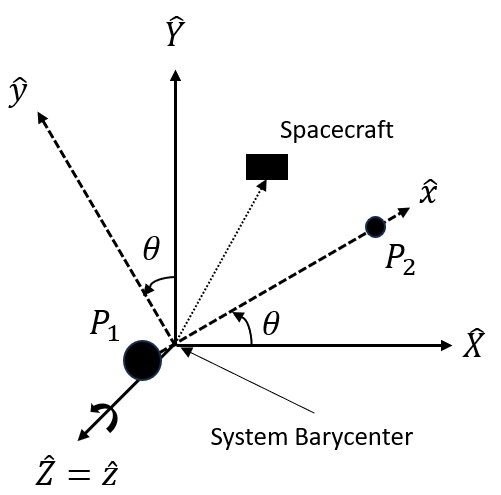
\includegraphics[width=0.5\textwidth]{figures/BaryFrames.jpg}
    \caption{Barycentric rotating and inertial frames in a CR3BP system.}
    \label{fig:baryFrames}
\end{figure}

\subsection{The Ecliptic J2000 Primary-Centered Inertial Frame}
A commonly used primary-centered inertial frame is the Ecliptic J2000. As the name implies, this
frame is established with its origin at the center of a primary body, and the Sun-Earth orbital
plane on January 1, 2000 as the $\Xhat_{Ec}\Yhat_{Ec}$-plane. The $\Xhat_{Ec}$-axis is directed
towards the vernal equinox, which is the line of intersection between the Earth's equatorial and
ecliptic planes on January 1, 2000. The $\Zhat_{Ec}$-axis is orthogonal to the ecliptic plane, and
the $\Yhat_{Ec}$-axis completes the triad, defined as $\Yhat_{Ec}=\Zhat_{Ec}\times\Xhat_{Ec}$.

Since the frame is centered on a primary, it is applicable to both the 2BP and CR3BP, making it
also valuable for patched dynamical models. The construction of this coordinate frame, as depicted
in \cref{fig:eclipJ2000Frame}, is computed using the Navigation and Ancillary Information
Facility's (NAIF) SPICE ephemeris toolkit\cite{Semenov:2023}.

\begin{figure}[ht]
    \centering
    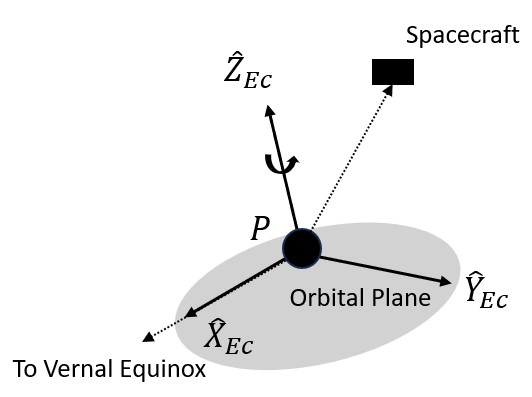
\includegraphics[width=0.5\textwidth]{figures/EclipJ2000Frame.jpg}
    \caption{Earth-centered Ecliptic J2000 inertial frame.}
    \label{fig:eclipJ2000Frame}
\end{figure}

\section{The Two-Body Problem}
This investigation treats the motion of spacecraft in heliocentric space, specifically when they
are far from planets and moons, as a Two-Body Problem, governed by a single gravitational force.
This section provides a brief overview of key aspects of 2BP dynamics, Keplerian orbital elements,
and Kepler's Equation. For a more comprehensive derivation of the 2BP, refer to Chapters 1 and 2 of
Vallado's \emph{Fundamentals of Astrodynamics and Applications}\cite{Vallado:2013}. Additionally,
Canales highlights the background information relevant to understanding the transfer methodologies
presented in this analysis\cite{Canales:2021}.

\subsection{Equations of Motion}
The 2BP involves two point masses\textemdash a primary body and a spacecraft\textemdash that exert
gravitational forces on each other. Since no external forces act on this system, the center of mass
of the bodies moves at a constant velocity and serves as the origin for an inertial coordinate
frame. In this inertial frame, the gravitational force that the primary body exerts on the
spacecraft, denoted as $\Fbar_{g_{P\rightarrow s/c}}$, is expressed as:
\begin{equation}
    \Fbar_{g_{P\rightarrow s/c}}=-\frac{Gm_{P}m_{s/c}}{r_{P\rightarrow s/c}^{3}}\rbar_{P\rightarrow s/c},
    \label{eq:gravity}
\end{equation}
where $G$ is the universal gravitational constant (6.67384x10$^{-20}$ kN*km$^{2}$/kg$^{2}$),
$m_{P}$ and $m_{S}$ are the masses of the primary body and spacecraft, respectively,
$r_{P\rightarrow s/c}$ is the distance from the primary body to the spacecraft, and
$\rbar_{P\rightarrow s/c}=\rbar_{s/c}-\rbar_{P}$ is the position vector from the primary body to
the spacecraft in the inertial frame, as illustrated in \cref{fig:2BP}.

\begin{figure}[ht]
    \centering
    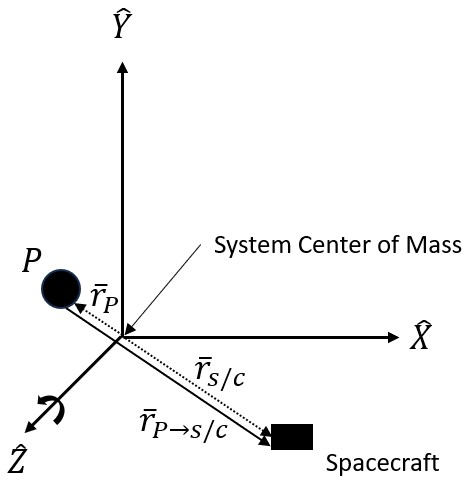
\includegraphics[width=0.5\textwidth]{figures/TBP.jpg}
    \caption{Two-body problem in a barycentric inertial frame.}
    \label{fig:2BP}
\end{figure}

Assuming that the mass of the spacecraft is negligible compared to the mass of the primary body,
the nonlinear relative equation of motion for the 2BP is derived\cite{Vallado:2013, Canales:2021}:
\begin{equation}
    \rbarddot_{P\rightarrow s/c}=-\frac{\mu_{2BP}}{r_{P\rightarrow s/c}^{3}}\rbar_{P\rightarrow s/c},
    \label{eq:TBPEoM}
\end{equation}
where $\rbarddot_{P\rightarrow s/c}$ is the inertial acceleration of the spacecraft relative to the
primary body and $\mu_{2BP}=Gm_{P}$. This vector equation can also be expressed as $\Xhat$,
$\Yhat$, and $\Zhat$ scalar equations in the inertial frame:
\begin{equation}
    \Xddot=-\frac{\mu_{2BP}}{r_{P\rightarrow s/c}^{3}}(X_{s/c}-X_{P}),
    \label{eq:TBPEoMX}
\end{equation}
\begin{equation}
    \Yddot=-\frac{\mu_{2BP}}{r_{P\rightarrow s/c}^{3}}(Y_{s/c}-Y_{P}),
    \label{eq:TBPEoMY}
\end{equation}
\begin{equation}
    \Zddot=-\frac{\mu_{2BP}}{r_{P\rightarrow s/c}^{3}}(Z_{s/c}-Z_{P}).
    \label{eq:TBPEoMZ}
\end{equation}

\subsection{Conic Sections}
Instead of relying on numerical propagation of the nonlinear equations of motion, spacecraft motion
in the 2BP can be effectively represented analytically using conic sections. This section provides
a concise overview of conic motion in the 2BP.

Two essential constants characterize conic orbits: specific angular momentum $\ambar$ and specific
mechanical energy $\mathcal{E}$:
\begin{equation}
    \ambar=\rbar_{P\rightarrow s/c}\times\rbardot_{P\rightarrow s/c},
    \label{eq:angularmomentum}
\end{equation}
\begin{equation}
    \mathcal{E}=\frac{v_{P\rightarrow s/c}^{2}}{2}-\frac{\mu_{2BP}}{r_{P\rightarrow s/c}},
    \label{eq:energy}
\end{equation}
where $v_{P\rightarrow s/c}=||\rbardot_{P\rightarrow s/c}||_{2}$ is the spacecraft velocity in the
inertial frame relative to the primary body.

Kepler's first law, asserting that orbital motion is conic, provides the trajectory equation for
the 2BP:
\begin{equation}
    r_{P\rightarrow s/c}=\frac{a(1-e^{2})}{1+e\cos(\theta)},
    \label{eq:trajectory}
\end{equation}
where $a$ represents the orbit semimajor axis, $e$ is the orbit eccentricity, and $\theta$ denotes
the orbit true anomaly. These three elements will be elaborated upon in a later subsection.
\cref{eq:trajectory} can also be employed to compute the periapsis and apoapsis distances, $r_{p}$
and $r_{a}$ respectively:
\begin{equation}
    r_{p}=a(1-e),
    \label{eq:periapsis}
\end{equation}
\begin{equation}
    r_{a}=a(1+e).
    \label{eq:apoapsis}
\end{equation}

The eccentricity can also be used to determine the type of conic section:
\begin{itemize}
    \item   $e=0$: Circular orbit (a special case of an ellipse).
    \item   $0<e<1$: Elliptical orbit.
    \item   $e=1$: Parabola.
    \item   $e>1$: Hyperbola.
\end{itemize}
This investigation focuses on circles and ellipses with $0\leq e<1$.

Similarly, Kepler's third law provides the orbit period $\mathbb{P}$ and, consequently, the mean
motion $n$:
\begin{equation}
    \mathbb{P}=2\pi\sqrt{\frac{a^{3}}{\mu_{2BP}}},
    \label{eq:period}
\end{equation}
\begin{equation}
    n=\frac{2\pi}{\mathbb{P}}=\sqrt{\frac{\mu_{2BP}}{a^{3}}}.
    \label{eq:meanmotion}
\end{equation}

\subsection{Keplerian Orbital Elements}
Instead of specifying the six-dimensional state of a spacecraft in a 2BP elliptical orbit using
Cartesian coordinates, six orbital elements can be employed to articulate the size, shape,
orientation, and current location along the orbit. In addition to the semimajor axis $a$ and
eccentricity $e$, which were introduced earlier and describe the size and shape of the ellipse,
three angles characterize the orientation of the orbit with respect to an inertial frame, as
depicted in \cref{fig:orbitalElements}:
\begin{itemize}
    \item \textbf{Inclination} $i$ signifies the tilt of the orbital plane relative to the inertial
    $\Xhat_{Ec}\Yhat_{Ec}$-plane.
    \item \textbf{Right ascension of the ascending node} (RAAN) $\Omega$ denotes the angle between
    the $\Xhat_{Ec}$-axis and the ascending node, where the orbit crosses the
    $\Xhat_{Ec}\Yhat_{Ec}$-plane in the positive $\Zhat_{Ec}$ direction.
    \item \textbf{Argument of periapsis} $\omega$ is the angle between the ascending node and the
    periapsis.
\end{itemize}
Finally, the true anomaly $\theta$ defines the spacecraft's position relative to the orbit's
periapsis.

\begin{figure}[ht]
    \centering
    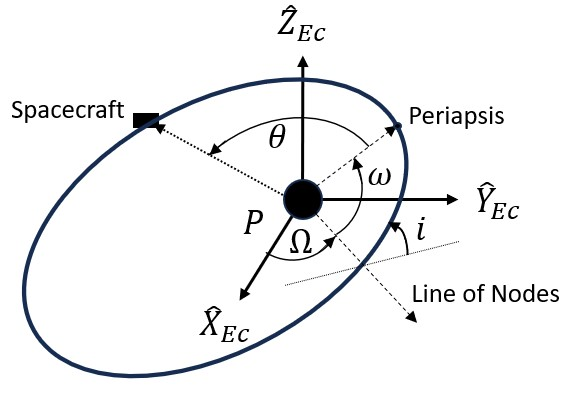
\includegraphics[width=0.5\textwidth]{figures/OrbitalElements.jpg}
    \caption{Orientation and location along an orbit in an inertial frame using Keplerian orbital elements.}
    \label{fig:orbitalElements}
\end{figure}

\subsubsection{Cartesian state to Keplerian orbital elements}
To convert from a Cartesian state vector to Keplerian orbital elements, start by calculating the
inclination from angular momentum:
\begin{equation}
    i=\arccos(\frac{h_{Z}}{||\ambar||})
    \label{eq:inclination}
\end{equation}
Using the node vector $\nbar$:
\begin{equation}
    \nbar=\Zhat_{Ec}\times\ambar,
    \label{eq:nodes}
\end{equation}
the RAAN becomes:
\begin{equation}
    \Omega=\begin{cases}\arccos(\frac{n_{X}}{||\nbar||})&n_{Y}\geq0\cr2\pi-\arccos(\frac{n_{X}}{||\nbar||})&n_{Y}<0\end{cases}.
    \label{RAAN}
\end{equation}
The eccentricity vector $\ebar$ is also calculated from the angular momentum:
\begin{equation}
    \ebar=\frac{\rbardot_{P\rightarrow s/c}\times\ambar}{\mu_{2BP}}-\frac{\rbar_{P\rightarrow s/c}}{r_{P\rightarrow s/c}},
    \label{eq:eccentricityvector}
\end{equation}
and
\begin{equation}
    e=||\ebar||.
    \label{eq:eccentricity}
\end{equation}
The remaining three orbital elements are calculated as follows:
\begin{equation}
    a=\frac{||\ambar||}{\mu_{2BP}(1-e^{2})},
    \label{eq:semimajoraxis}
\end{equation}
\begin{equation}
    \omega=\begin{cases}\arccos(\frac{\nbar\cdot\ebar}{||\nbar||e})&e_{Z}\geq0\cr2\pi-\arccos(\frac{\nbar\cdot\ebar}{||\nbar||e})&e_{Z}<0\end{cases},
    \label{eq:argumentofperiapsis}
\end{equation}
\begin{equation}
    \theta=\begin{cases}\arccos(\frac{\ebar\cdot\rbar_{P\rightarrow s/c}}{er_{P\rightarrow s/c}})&v_{r}\geq0\cr2\pi-\arccos(\frac{\ebar\cdot\rbar_{P\rightarrow s/c}}{er_{P\rightarrow s/c}})&v_{r}<0\end{cases},
    \label{eq:trueanomaly}
\end{equation}
where
\begin{equation}
    v_{r}=\frac{\rbardot_{P\rightarrow s/c}\cdot\rbar_{P\rightarrow s/c}}{r_{P\rightarrow s/c}}.
    \label{eq:radialvelocity}
\end{equation}

\subsubsection{Keplerian orbital elements to Cartesian state}
Similarly, the Cartesian state vector can be obtained from the Keplerian orbital elements. First,
the eccentric anomaly $E$ is needed, which is the angle made by the eccentricity vector pointing to
periapsis and the vector from the center of the ellipse to the point directly above the spacecraft
location (perpendicular to the eccentricity vector) on an auxiliary circle drawn tangent to the
ellipse. The eccentric anomaly and the auxiliary circle are illustrated in \cref{fig:auxCircle}, along
with the eccentricity vector and semimajor axis.

\begin{figure}[ht]
    \centering
    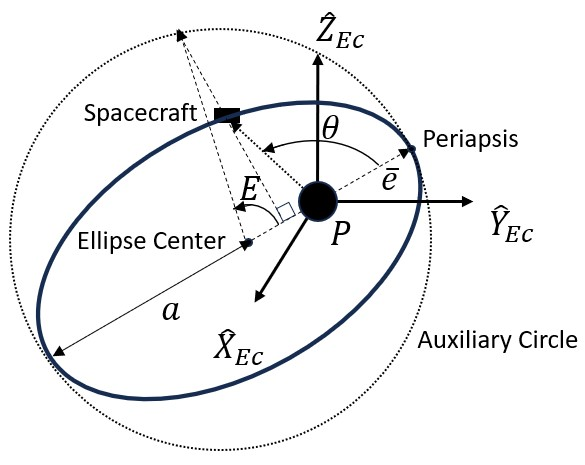
\includegraphics[width=0.5\textwidth]{figures/AuxCircle.jpg}
    \caption{Definition of eccentric anomaly and the auxiliary circle.}
    \label{fig:auxCircle}
\end{figure}

The eccentric anomaly can be related to the true anomaly,
\begin{equation}
    E=\arctan(\frac{\sqrt{1-e^{2}}\sin(\theta)}{e+\cos(\theta)}),
    \label{eq:eccentricanomaly}
\end{equation}
which can then be used to calculate the distance from the primary:
\begin{equation}
    r_{P\rightarrow s/c}=a(1-e\cos(E)).
    \label{eq:circularradius}
\end{equation}
This can be used to generate position and velocity magnitude vectors:
\begin{equation}
    \rbar_{0}=\begin{bmatrix}r_{P\rightarrow s/c}\cos(\theta)\cr r_{P\rightarrow s/c}\sin(\theta)\cr0\end{bmatrix},
    \label{eq:circularpositionvector}
\end{equation}
\begin{equation}
    \rbardot_{0}=\sqrt{\frac{\mu_{2BP}a}{r_{P\rightarrow s/c}}}\begin{bmatrix}-\sin(E)\cr\sqrt{1-e^{2}}\cos(E)\cr0\end{bmatrix}.
    \label{eq:circularvelocityvector}
\end{equation}
These vectors will need to be rotated relative to the inertial frame axes according to the
inclination, RAAN, and argument of periapsis:
\begin{equation}
    C=\begin{bmatrix}\cos(\Omega)\cos(\omega)-\cos(i)\sin(\Omega)\sin(\omega)&-\cos(\Omega)\sin(\omega)-\cos(i)\sin(\Omega)\cos(\omega)&0\cr\sin(\Omega)\cos(\omega)+\cos(i)\cos(\Omega)\sin(\omega)&-\sin(\Omega)\sin(omega)+\cos(i)\cos(\Omega)\cos(\omega)&0\cr\sin(i)\sin(\omega)&\sin(i)\cos(\omega)&0\end{bmatrix},
    \label{eq:elementrotation}
\end{equation}
\begin{equation}
    \rbar_{P\rightarrow s/c}=C\rbar_{0},
    \label{eq:positionvector}
\end{equation}
\begin{equation}
    \rbardot_{P\rightarrow s/c}=C\rbardot_{0}.
    \label{eq:velocityvector}
\end{equation}

\subsection{Kepler's Equation}
If the difference in true anomaly between two points on an orbit is known, Kepler's equation
becomes a valuable tool for calculating the time-of-flight between these points. The mean anomaly
$M$ serves as a measure of how much of the orbit has been traversed past periapsis with respect to
time:
\begin{equation}
    M=\frac{2\pi(t-t_{p})}{\mathbb{P}},
    \label{eq:meananomaly}
\end{equation}
where $(t-t_{p})$ represents the time since periapsis.

Kepler's equation establishes a connection between the mean and eccentric anomalies, thereby
linking the eccentric anomaly to time:
\begin{equation}
    M=E-e\sin(E).
    \label{eq:Keplersequation}
\end{equation}

To determine eccentric anomalies given corresponding true anomalies, employ
\cref{eq:eccentricanomaly}, and subsequently, using Kepler's equation (\cref{eq:Keplersequation}),
convert them to mean anomalies. The difference in mean anomalies with \cref{eq:meananomaly}
provides the time-of-flight between the two points along the orbit.

\section{The Circular Restricted Three-Body Problem}
\section{Patched Dynamical Models}
A variety of methods exist to model the gravitational forces of three (or more) celestial bodies in
dynamical systems. While a high-fidelity ephemeris model (HFEM) provides the best accuracy, some
models utilize simplifying assumptions to reduce computations and gain more insight into the
dynamics of the system while maintaining adequate fidelity. For including all of the bodies in one
model, there exist several 4-body problems that differ in layout, coherency, and fidelity. Some of
the more prominent options are the (BCR4BP)\cite{Boudad:2018}, Hills restricted 4-body problem
(HR4BP)\cite{Scheeres:1998}, and quasi-bicircular restricted 4-body problem
(QBCR4BP)\cite{Andreu:2002}. A different approach, and the one used in this investigation, is to
patch together 2BP and CR3BP models to build a larger model to represent the dynamics. Two such
patched models are outlined here.

\subsection{The Patched 2BP-CR3BP Model}
A patched 2BP-CR3BP model is used to describe trajectories as they move between CR3BP systems via a
2BP system. An example from this investigation is leaving the Sun-Earth CR3BP into heliocentric
space (modeled as a 2BP) before entering the Sun-Mars CR3BP. While the spacecraft is near a planet,
it is modeled in the Sun-planet CR3BP. But once it reaches a specified distance from that planet,
it is modeled instead using Keplearian 2BP motion around the Sun\cite{Canales:2021b}. The interface
location between the two models is called the sphere of influence (SoI) since it represents where
the gravitational influence of the planet becomes negligible compared to that of the Sun.

Trajectories computed in this model are best represented by using a coordinate frame centered on
the focus of the 2BP, the Sun in this example. In this investigation, trajectories in the 2BP-CR3BP
patched model are shown in the Sun-centered Ecliptic J2000 Frame, as described in Section 2.1.2.
Although the Sun-Earth CR3BP is coplanar with this frame, the Sun-Mars CR3BP system is not and Mars
is considered to be located at its respective orbital inclination. The $XY$-projection of an
example 2BP-CR3BP patched model system is shown in \cref{fig:2BP-CR3BP}.

\begin{figure}[ht]
    \centering
    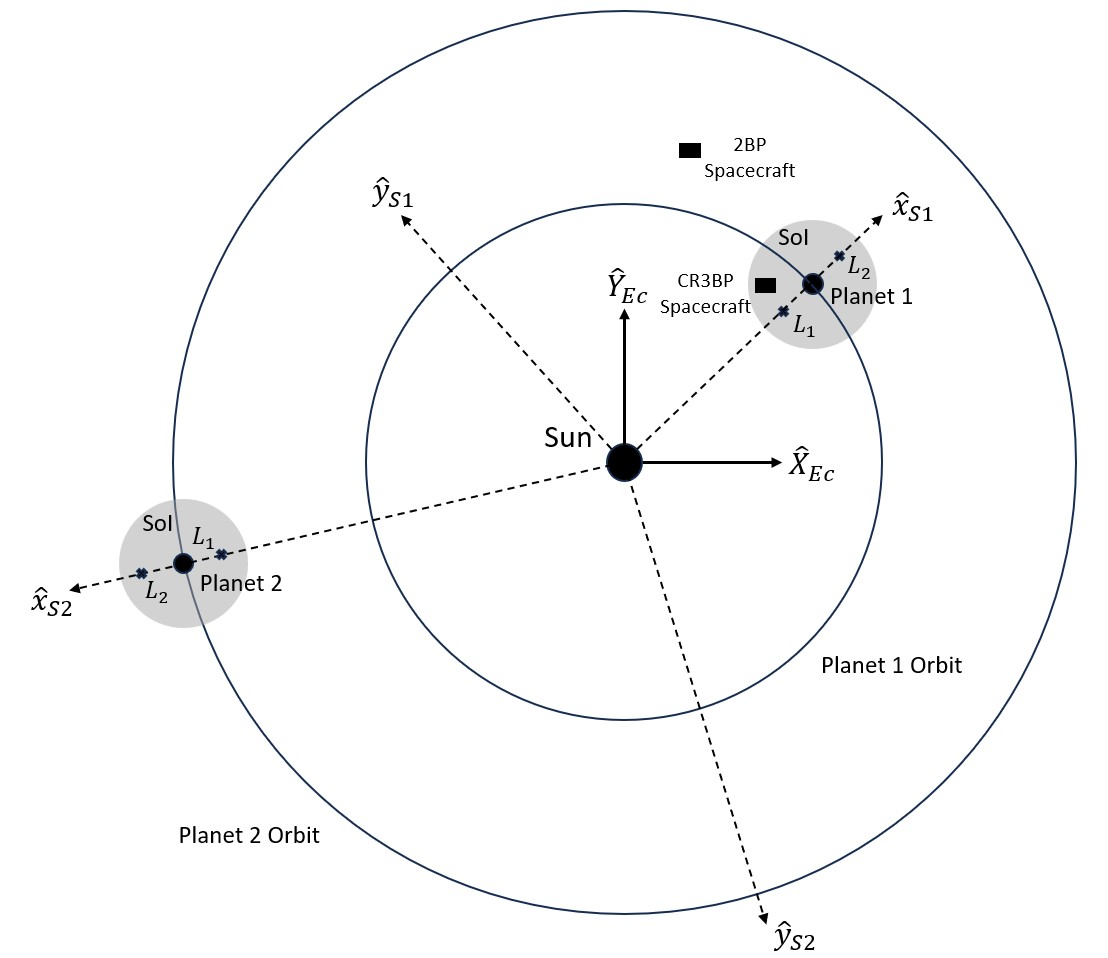
\includegraphics[width=0.75\textwidth]{figures/TBP-CR3BP.jpg}
    \caption{$XY$-Projection of the Patched 2BP-CR3BP Model}
    \label{fig:2BP-CR3BP}
\end{figure}

The radius of the SoI is a design parameter dependent on the application. For this patched model,
an SoI is desired such that CR3BP periodic orbits around the Lagrange points are included,
demonstrated in \cref{fig:SoI}. By defining a gravitational ratio:
\begin{equation}
    d_{SoI}=\frac{g_{2}}{g_{1}},
    \label{eq:patchedSoI}
\end{equation}
where $g_{i}$ is the gravitational acceleration of the respective primary body at a specified
location, an SoI radius from the planet can be chosen so that $d_{SoI}$ is sufficiently small,
i.e., the osculating (instantaneous) orbital elements remain near constant in the
CR3BP\cite{Canales:2021b}.

\begin{figure}[ht]
    \centering
    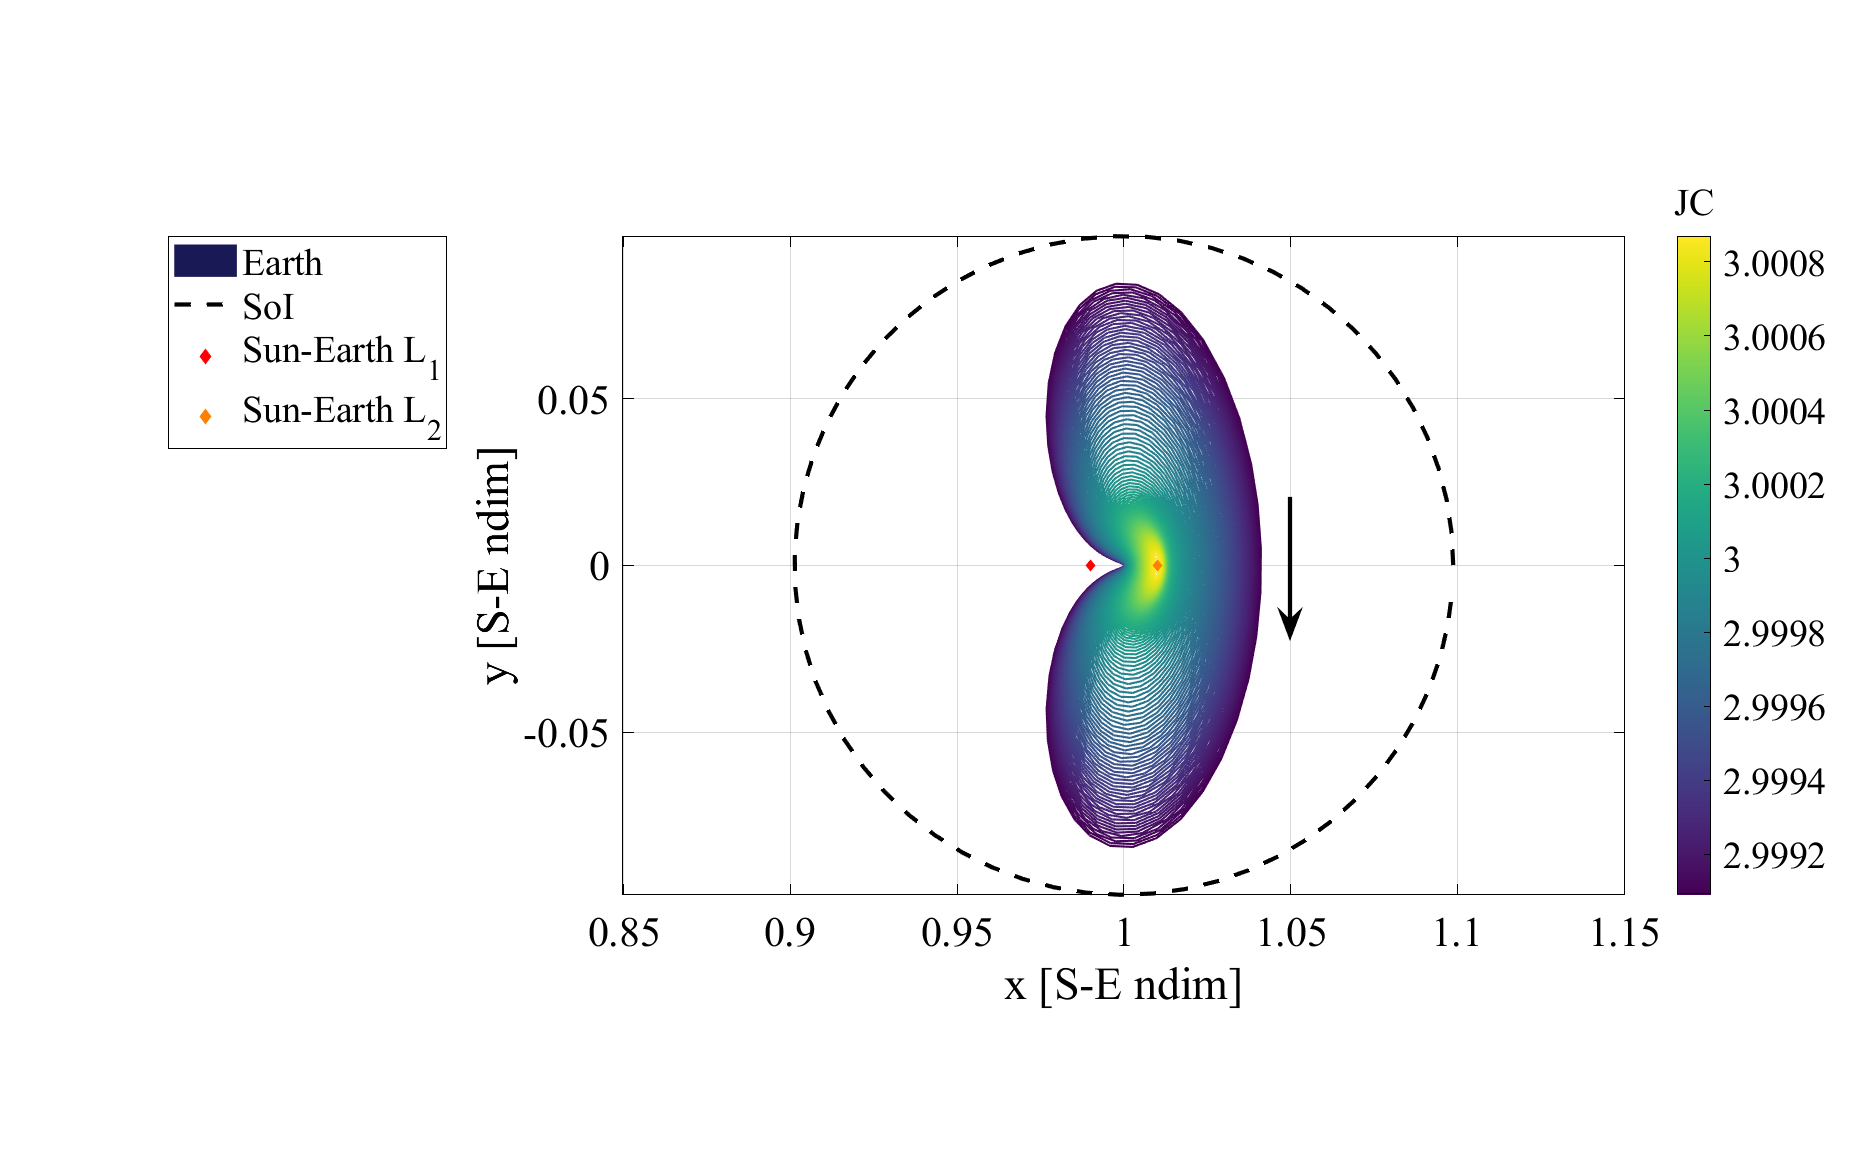
\includegraphics[width=0.9\textwidth]{figures/SoI.pdf}
    \caption{Patched 2BP-CR3BP sphere of influence around Earth, encompassing a large portion of the Sun-Earth $L_{2}$ Lyapunov family.}
    \label{fig:SoI}
\end{figure}

\subsection{The Blended CR3BP Model}
Two CR3BP models can be blended to form a 4-body model if one of the primary bodies is present in
both models. For example, a Sun-Earth CR3BP can be blended with an Earth-Moon CR3BP to form a
Sun-Earth-Moon 4-body problem (here, the Earth is the common primary). This method incorporates the
difference in inclinations between the two CR3BP models but is now a time-dependent
model\cite{Kakoi:2014}. Similar to the patched 2BP-CR3BP model, the boundary between the two models
is at an SoI, now around the smaller primary of the smaller CR3BP model (the Moon in this example).

Unlike the patched model above, this model is best represented in the barycentric rotating frame of
the larger CR3BP model (the Sun-Earth rotating frame in this example). Since the blended model is
time-dependent, the portion of the trajectory computed in the smaller CR3BP will be shifted when
represented in the larger model depending on the epoch. The $xy$-projection of an example blended
system is shown in \cref{fig:BlendedCR3BP}.

\begin{figure}[ht]
    \centering
    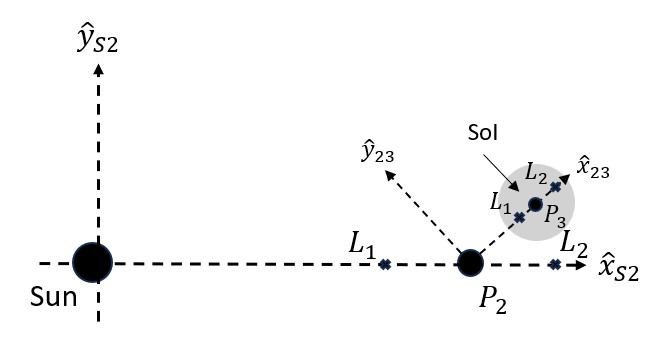
\includegraphics[width=0.5\textwidth]{figures/BlendCR3BP.jpg}
    \caption{$xy$-Projection of the Blended CR3BP Model}
    \label{fig:BlendedCR3BP}
\end{figure}

The SoI radius used for the blended model is different from that used for the patched model. As
mentioned before, this SoI is centered around the second primary of the smaller system and the
gravitational accelerations being compared are the first primary of the larger system and the
smaller primary of the second system (e.g., the Sun and the Moon). A blended CR3BP SoI radius is
defined as:
\begin{equation}
    r_{SoI}=l^{*}_{12}(\frac{m_{3}}{m_{1}})^{2/5},
    \label{eq:blendedSoI}
\end{equation}
where the primaries are numbered in order of decreasing mass\cite{Parker:2013}.

\section{Coordinate Frame Transformations}
Since the patched and blended models used in this investigation use a variety of models centered
around different bodies, it is helpful to be able to view any trajectories in multiple reference
frames. As mentioned previously, reference frames can be inertial or rotating, and an important
component of interplanetary trajectory design is the ability to transform states and trajectories
between these two types of frames. A few representative example coordinate frame transformations
follow.

\subsection{Barycentric Rotating Frame - Primary-Centric Arbitrary Inertial Frame}
Most trajectories in a CR3BP are constructed in the barycentric rotating frame where
\cref{eq:EoMx}-\cref{eq:EoMz} are defined (see \cref{fig:baryFrames}). However, it can also be
beneficial to view these in an inertial frame centered on one of the primary gravitational bodies.
An arbitrary inertial frame can be defined where the inertial unit vectors $\{\Xhat,\Yhat,\Zhat\}$
are equivalent to the rotating unit vectors $\{\xhat,\yhat,\zhat\}$ at time $t_{0}$ (although the
frame centers may be in different locations).

The following steps will transform (nondimensionalized) states from the barycentric rotating frame
to a primary-centric arbitrary inertial frame:

\begin{enumerate}
    \item   Translate the position states from barycentric to primary-centric:
            \begin{equation}
                \rhobar_{P\rightarrow s/c}=\rhobar_{s/c}-\rhobar_{P}.
                \label{eq:translation}
            \end{equation}
    \item   Rotate the states depending on time since $t_{0}$
    
            Recall that the mean motion $n$ of the rotating frame is constant. When
            nondimensionalized in the CR3BP, $\ntilde=1$ and therefore the rtoation angle is just
            $\tau-\tau_{0}$. Since the $\zhat$- and $\Zhat$-axes coincide for an arbitrary inertial
            frame, a simple rotation matrix can be used to rotate the position states:
            \begin{equation}
                \Pbar=\begin{bmatrix}   \cos(\tau-\tau_{0}) &   -\sin(\tau-\tau_{0})    &   0   \\
                                        \sin(\tau-\tau_{0}) &   \cos(\tau-\tau_{0})     &   0   \\
                                        0                   &   0                       &   1   \end{bmatrix}\rhobar=\prescript{I}{}{C}^{R}\rhobar,
                \label{eq:positionrotation}
            \end{equation}
            where $\rhobar$ is the rotating position and $\Pbar$ is the inertial position.

            Basic kinematics can be used to compute the velocity in the rotating frame relative to
            an inertial observer:
            \begin{equation}
                \frac{\prescript{I}{}{d\rhobar}}{d\tau}=\frac{\prescript{R}{}{d\rhobar}}{d\tau}+\prescript{I}{}{\omegabar}^{R}\times\rhobar=\rhobardot+\zhat\times\rhobar,
                \label{eq:BKE}
            \end{equation}
            where $\prescript{I}{}{\omegabar}^{R}=\ntilde\zhat$ is the angular velocity relating
            the two frames. Therefore:
            \begin{equation}
                \frac{\prescript{I}{}{d\rhobar}}{d\tau}=(\xdot-y)\xhat+(\ydot+x)\yhat+\zdot\zhat.
                \label{eq:inertialrotatingvelocity}
            \end{equation}
            
            Using the rotation matrix $\prescript{I}{}{C}^{R}$ from \cref{eq:positionrotation},
            \cref{eq:inertialrotatingvelocity} can be written in matrix from and combined with the
            position rotation to achieve full state rotation:
            \begin{equation}
                \Qbar=\begin{bmatrix}   \prescript{I}{}{C}^{R}      &   \zerobar                \\
                                        \prescript{I}{}{\dot{C}}^{R} &   \prescript{I}{}{C}^{R}  \end{bmatrix}\qbar,
                \label{eq:rotation}
            \end{equation}
            where $\qbar$ is the rotating state and $\Qbar$ is the inertial state.
    \item   Dimensionalize the states if desired (see Section 2.3.2).
\end{enumerate}

To transform a primary-centric arbitrary inertial state to a barycentric rotating state, just
reverse the above states (nondimensionalizing if necessary) and invert the state rotation matrix.

\subsection{Barycentric Rotating Frame - Ecliptic J2000 Inertial Frame}
When desigining a trajectory across multiple systems, it is often useful to view each part of the
trajectory in a common inertial reference frame. In this investigation, the Earth Ecliptic J2000
inertial frame, introduced in Section 2.1.2 (\cref{fig:eclipJ2000Frame}), is used as the common
frame for interplanetary trajectories.

The transformation between barycentric rotating frame states and a primary-centric Ecliptic J2000
inertial frame states follows a similar process to the arbitrary inertial frame. However, since
this frame is defined by a particular epoch (January 1, 2000), the frame rotation is
epoch-dependent:

\begin{enumerate}
    \item   To properly compare the rotating frame to the Ecliptic J2000 inertial frame, the
            location of the second primary in its orbit at each epoch of the trajectory is needed.
            This is obtained by retrieving the orbital elements of the second primary at a selected
            initial epoch from SPICE\cite{Semenov:2023}. These orbital elements are then modified
            to match the CR3BP orbit assumptions ($a=l^{*}$ and $e=0$). Since the mean
            motion/angular velocity in the CR3Bp is constant at $\ntilde=1$:
            \begin{equation}
                \theta=\tau-\tau_{0}+\theta_{0},
                \label{eq:instantaneoustrueanomaly}
            \end{equation}
            where $\theta_{0}$ is the true anomaly at the initial epoch $t-{0}$ obtained from
            SPICE. These updated orbital elements are then used to calculate the full state vector
            (in dimensional units) of the second primary relative to the first using
            \cref{eq:eccentricanomaly}-\cref{eq:velocityvector}.
    \item   Dimensionalize the trajectory states, times, and angular velocity (see Section 2.3.2).
    \item   At each time, translate the position states from barycentric to primary-centric using
            \cref{eq:translation} (note that dimensional values should be used).
    \item   Define the instantaneous state rotation matrix using the second primary's Ecliptic
            J2000 state vector and angular momentum $\ambar$ (\cref{eq:angularmomentum}) at each
            time:
            \begin{equation}
                \xhat=\frac{\Rbar_{P_{1}\rightarrow P_{2}}}{|\Rbar_{P_{1}\rightarrow P_{2}}|},
                \label{eq:xhat}
            \end{equation}
            \begin{equation}
                \zhat=\frac{\ambar}{|\ambar|},
                \label{eq:zhat}
            \end{equation}
            \begin{equation}
                \yhat=\zhat\times\xhat,
                \label{eq:yhat}
            \end{equation}
            \begin{equation}
                \prescript{Ec}{}{C}^{R}=\begin{bmatrix} \xhat   &   \yhat   &   \zhat   \end{bmatrix}.
                \label{eq:eclipticpositionrotation}
            \end{equation}

            The full state rotation matrix can be found through the same process used in Section
            2.5.1, using a dimensional angular velocity:
            \begin{equation}
                \prescript{Ec}{}{\dot{C}}^{R}=\begin{bmatrix}   n\yhat  &   -n\xhat &   \zerobar    \end{bmatrix}.
                \label{eq:eclipticvelocityrotation}
            \end{equation}
            in \cref{eq:rotation} with dimensional values.
    \item   Nondimensionalize the states if desired.
\end{enumerate}

States can be transformed from a primary-centric Ecliptic J2000 inertial frame to a barycentric
rotating frame by reversing the above steps and inverting the state rotation matrix. This
becomes a useful tool when designing interplanetary trajectories using multi-body dynamics.


\chapter{CR3BP DYNAMICAL STRUCTURES}

As mentioned in the previous chapter, there is no analytical solution to the CR3BP. Instead,
trajectories are propagated using numerical methods. Various numerical techniques are applied to
find existing dynamical structures in the model, such as periodic orbits and invariant manifolds,
and obtain corresponding initial conditions for propagation. These include differential
corrections, natural parameter continuation, eigen decomposition, and Poincar\'e mapping.

\section{Differential Corrections}
Differential corrections are used to compute solutions in targeting problems that satisfy the
provided constraints on the initial condition and the trajectory arc. To do so, it is necessary to
be able to relate downstream states to the initial condition.

\subsection{State Transition Matrix}
The state transition matrix (STM) relates variations in an initial state, $\qbar_{0}=\qbar(t_{0})$,
to variations in a downstream state $\qbar(t)$. Starting from a first-order Taylor series expansion
about the baseline trajectory arc, the linear variational equation is derived:
\begin{equation}
    \partial\qbardot(t)=A(t)\partial\qbar(t),
    \label{eq:linearvariational}
\end{equation}
where $A(t)$ is the Jacobian matrix for the equations of motion with respect to the state at time
$t$. A full derivation for the CR3BP $A(t)$ matrix can be found in Zimovan, but the result is given
here\cite{Zimovan:2017}:
\begin{equation}
    A(t)=\begin{bmatrix}    \frac{\partial x}{\partial x_{0}}       &   \frac{\partial x}{\partial y_{0}}       &   \frac{\partial x}{\partial z_{0}}       &   \frac{\partial x}{\partial \xdot_{0}}       &   \frac{\partial x}{\partial \ydot_{0}}       &   \frac{\partial x}{\partial \zdot_{0}}       \\
                            \frac{\partial y}{\partial x_{0}}       &   \frac{\partial y}{\partial y_{0}}       &   \frac{\partial y}{\partial z_{0}}       &   \frac{\partial y}{\partial \xdot_{0}}       &   \frac{\partial y}{\partial \ydot_{0}}       &   \frac{\partial y}{\partial \zdot_{0}}       \\
                            \frac{\partial z}{\partial x_{0}}       &   \frac{\partial z}{\partial y_{0}}       &   \frac{\partial z}{\partial z_{0}}       &   \frac{\partial z}{\partial \xdot_{0}}       &   \frac{\partial z}{\partial \ydot_{0}}       &   \frac{\partial z}{\partial \zdot_{0}}       \\
                            \frac{\partial \xdot}{\partial x_{0}}   &   \frac{\partial \xdot}{\partial y_{0}}   &   \frac{\partial \xdot}{\partial z_{0}}   &   \frac{\partial \xdot}{\partial \xdot_{0}}   &   \frac{\partial \xdot}{\partial \ydot_{0}}   &   \frac{\partial \xdot}{\partial \zdot_{0}}   \\
                            \frac{\partial \ydot}{\partial x_{0}}   &   \frac{\partial \ydot}{\partial y_{0}}   &   \frac{\partial \ydot}{\partial z_{0}}   &   \frac{\partial \ydot}{\partial \xdot_{0}}   &   \frac{\partial \ydot}{\partial \ydot_{0}}   &   \frac{\partial \ydot}{\partial \zdot_{0}}   \\
                            \frac{\partial \zdot}{\partial x_{0}}   &   \frac{\partial \zdot}{\partial y_{0}}   &   \frac{\partial \zdot}{\partial z_{0}}   &   \frac{\partial \zdot}{\partial \xdot_{0}}   &   \frac{\partial \zdot}{\partial \ydot_{0}}   &   \frac{\partial \zdot}{\partial \zdot_{0}}   \end{bmatrix}
        =\begin{bmatrix}    0                                       &   0                                       &   0                                       &   1   &   0   &   0   \\
                            0                                       &   0                                       &   0                                       &   0   &   1   &   0   \\
                            0                                       &   0                                       &   0                                       &   0   &   0   &   1   \\
                            \frac{\partial U}{\partial x\partial x} &   \frac{\partial U}{\partial x\partial y} &   \frac{\partial U}{\partial x\partial z} &   0   &   2n  &   0   \\
                            \frac{\partial U}{\partial y\partial x} &   \frac{\partial U}{\partial y\partial y} &   \frac{\partial U}{\partial y\partial z} &   -2n &   0   &   0   \\
                            \frac{\partial U}{\partial z\partial x} &   \frac{\partial U}{\partial z\partial y} &   \frac{\partial U}{\partial z\partial z} &   0   &   0   &   0   \end{bmatrix},
                            \label{eq:variationalJacobian}
\end{equation}
\begin{equation}
    \frac{\partial U}{\partial x\partial x}=1-\frac{1-\mu}{d^{3}}-\frac{\mu}{r^{3}}+\frac{3(1-\mu)(x+\mu)^{2}}{d^{5}}+\frac{3\mu(x-1+\mu)^{2}}{r^{5}},
    \label{eq:partialUpartialxx}
\end{equation}
\begin{equation}
    \frac{\partial U}{\partial x\partial y}=\frac{\partial U}{\partial y\partial x}=\frac{3(1-\mu)(x+\mu)y}{d^{5}}+\frac{3\mu(x-1+\mu)y}{r^{5}},
    \label{eq:partialUpartialxy}
\end{equation}
\begin{equation}
    \frac{\partial U}{\partial x\partial z}=\frac{\partial U}{\partial z\partial x}=\frac{3(1-\,u)(x+\mu)z}{d^{5}}+\frac{3\mu(x-1+\mu)z}{r^{5}},
    \label{eq:partialUpartialxz}
\end{equation}
\begin{equation}
    \frac{\partial U}{\partial y\partial y}=1-\frac{1-\mu}{d^{3}}-\frac{\mu}{r^{3}}+\frac{3(1-\mu)y^{2}}{d^{5}}+\frac{3\mu y^{2}}{r^{5}},
    \label{eq:partialUpartialyy}
\end{equation}
\begin{equation}
    \frac{\partial U}{\partial y\partial z}=\frac{\partial U}{\partial z\partial y}=\frac{3(1-\mu)yz}{d^{5}}+\frac{3\mu yz}{r^{5}},
    \label{eq:partialUpartialyz}
\end{equation}
\begin{equation}
    \frac{\partial U}{\partial z\partial z}=-\frac{1-\mu}{d^{3}}-\frac{\mu}{r^{3}}+\frac{3(1-\mu)z^{2}}{d^{5}}+\frac{3\mu z^{2}}{r^{5}}.
    \label{eq:partialUpartialzz}
\end{equation}
The solution to \cref{eq:linearvariational}:
\begin{equation}
    \partial\qbar(t)=\frac{\partial\qbar(t)}{\partial\qbar_{0}}\partial\qbar_{0},
    \label{eq:variationalsolution}
\end{equation}
can be rearranged to provide the STM $\Phi(t,t_{0})$:
\begin{equation}
    \Phi(t,t_{0})=\frac{\partial\qbar(t)}{\partial\qbar_{{0}}}.
    \label{eq:STM}
\end{equation}
The equation of motion for the STM can be appended to the CR3BP equations of motion when
propagating:
\begin{equation}
    \dot{\Phi}(t,t_{0})=A(t)\Phi(t,t_{0}),
    \label{eq:STMEoM}
\end{equation}
where the initial condition is $\Phi(t_{0},t_{0})=I_{6\times6}$.

\subsection{Multi-Variable Newton-Raphson Method}
Targeting problems require iterative approaches where an initial guess is updated until it meets a
set of constraints to solve a boundary value problem. This investigation uses a multi-variable
Newton-Raphson method as a differential corrections process for single-shooting targeting problems,
applying analytical or numerical partial derivatives of constraints with respect to the initial
conditions.

If $\Xbar$ is the free variable vector and $\Fbar(\Xbar)$ is the constraint vector, dependent on
the free variables, then the goal of the targeting problem is to find $\Xbar$ such that
$\Fbar(\Xbar)=\zerobar$ (to a chosen tolerance). Example free variable and constraint vectors will
be introduced in future sections of this chapter and document. Under the Newton-Raphson method, the
update equation is again provided by a first-order Taylor series expansion about the initial
condition $\Xbar_{0}$:
\begin{equation}
    \Fbar(\Xbar)=\Fbar(\Xbar_{0})+DF(\Xbar_{0})(\Xbar-\Xbar_{0})=\zerobar,
    \label{eq:updateequation}
\end{equation}
where $DF(\Xbar)$ is the Jacobian matrix containing the partial derivatives of the constraint
vector with respect to the free variable vector.

With this update equation, the next iteration on the initial conditions can be computed. If the
number of free variables matches the number of constraints:
\begin{equation}
    \Xbar=\Xbar_{0}-DF(\Xbar_{0})^{-1}\Fbar(\Xbar_{0}),
    \label{eq:NRsolution}
\end{equation}
and this becomes the new iteration of the initial conditions. Ideally, upon each iteration, the
norm of the constraint vector should approach closer to the tolerance. If the number of free
variables is greater than the number of constraints, a minimum-norm solution can be used:
\begin{equation}
    \Xbar=\Xbar_{0}-DF(\Xbar_{0})^{T}(DF(\Xbar_{0})DF(\Xbar_{0})^{T})^{-1}\Fbar(\Xbar_{0}).
    \label{eq:minimumnorm}
\end{equation}
When the number of free variables is less than the number of constraints, a least squares solution
can be used, but that is not addressed in this investigation.

As a simple targeting example, consider the following planar boundary value problem in
\cref{fig:targeting}. The objective is to vary the initial velocity and time-of-flight (TOF) to
target a desired final position $\rhobar_{d}$. This results in a free variable vector:
\begin{equation}
    \Xbar=\begin{bmatrix}   \xdot_{0}   &   \ydot_{0}   &   \tau    \end{bmatrix}^{T},
    \label{eq:exfreevar}
\end{equation}
and constraint vector:
\begin{equation}
    \Fbar(\Xbar)=\begin{bmatrix}    x_{f}-x_{d} &   y_{f}-y_{d} \end{bmatrix}^{T}=\zerobar.
    \label{eq:exconst}
\end{equation}
The Jacobian matrix is comprised of the partial derivatives of the constraint vector with respect
to the free variable vector, in this case, a combination of the STM and time derivatives:
\begin{equation}
    DF(\Xbar)=\begin{bmatrix}   \frac{\partial(x_{f}-x_{d})}{\partial\xdot_{0}} &   \frac{\partial(x_{f}-x_{d})}{\partial\ydot_{0}} &   \frac{\partial(x_{f}-x_{d})}{\partial\tau}  \\
                                \frac{\partial(y_{f}-y_{d})}{\partial\xdot_{0}} &   \frac{\partial(y_{f}-y_{d})}{\partial\ydot_{0}} &   \frac{\partial(y_{f}-y_{d})}{\partial\tau}  \end{bmatrix}
             =\begin{bmatrix}   \phi_{14}                                       &   \phi_{15}                                       &   \xdot_{f}                                   \\
                                \phi_{24}                                       &   \phi_{25}                                       &   \ydot_{f}                                   \end{bmatrix},
    \label{eq:exJacobian}
\end{equation}
where $\phi$ are elements of the STM of the propagated arc. These vectors and the Jacobian matrix
can then be used in \cref{eq:minimumnorm} to iteratively solve for the free variable vector that
satisfies the constraint vector and solves the provided boundary value problem.

\begin{figure}[ht]
    \centering
    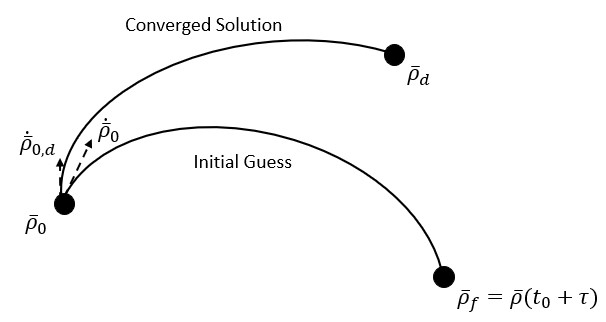
\includegraphics[width=0.75\textwidth]{figures/Targeting.jpg}
    \caption{Simple Targeting Example.}
    \label{fig:targeting}
\end{figure}

\subsection{Central Difference Method}
The Newton-Raphson method uses partial derivatives to solve a targeting problem iteratively. These
partial derivatives can be provided analytically (like in the previous example) or numerically
using an approximation method such as central differencing. The numerical approach is used in this
investigation to check analytical partial derivatives or when the analytical partials are overly
complicated.

The central difference method approximates the slope of the solution at discretized points just
before and after the initial condition:
\begin{equation}
    D\Fbar_{i}(\Xbar_{0})=\frac{\partial\Fbar(\Xbar_{0})}{\partial X_{i}}=\frac{\Fbar(X_{i}+\kappa)-\Fbar(X_{i}-\kappa)}{2\kappa},
    \label{eq:slope}
\end{equation}
where $X_{i}$ is one of the components of the free variable vector and $\kappa$ is a small
perturbation (this investigation uses the square root of the machine tolerance, $\sqrt{\epsilon}$).
Each variable in the free variable vector is perturbed in both directions by $\kappa$, one at a
time, and the constraint vector is evaluated at each new free variable vector and substituted into
\cref{eq:slope} above. Perturbing all of the free variables individually makes up the numerical
Jacobian matrix:
\begin{equation}
    DF(\Xbar_{0})=\begin{bmatrix}   D\Fbar_{1}(\Xbar_{0})   &   \dots   &   D\Fbar_{m}(\Xbar_{0})\end{bmatrix}.
    \label{eq:centraldifference}
\end{equation}
These numerical $DF$ matrices can be compared to their analytical counterparts (such as the example
Jacobian in \cref{eq:exJacobian}) to verify partial derivatives or applied in isolation when
analytical partial derivatives are either not available or exceedingly complex.

\section{Periodic Orbits}
Using the multi-variable Newton-Raphson scheme described above, periodic solutions can be targeted
in a CR3BP system. In the CR3BP, these periodic solutions exist as members of families that share
similar geometric characteristics. Some of these orbit families are symmetric about a plane or axis
in the rotating frame and this information can be utilized in the targeting process. In addition,
the initial conditions for these families can be obtained through a variety of methods including
linear variational equations about the Lagrange points and bifurcations from other orbit families.
All of the orbit families used in this investigation and shown here were selected for their
relative instability in the Earth-Moon CR3BP. For some example initial conditions for these orbit
families and others, see NASA Jet Propulsion Laboratory's CR3BP orbit database\cite{Park}.

\subsection{Lyapunov Orbits}
\phantomsection
\subsubsection{A Lyapunov Targeter}
To demonstrate the periodic orbit targeting process, the Newton-Raphson scheme will be used to
solve for a periodic orbit in the $xy$-plane of the rotating frame around the first Lagrange point.
This family of solutions is known as the $L_{1}$ Lyapunov family and they are symmetric about the
$xz$-plane. Therefore, instead of targeting the full orbit, it is only necessary to target half of
it, from one perpendicular crossing of the $xz$-plane to the next. To target one of these orbits at
a specified energy level (Jacobi constant), consider the free variable vector:
\begin{equation}
    \Xbar=\begin{bmatrix}   x_{0}   &   \ydot_{0}   &   \tau    \end{bmatrix}^{T}.
    \label{eq:Lyapunovfreevar}
\end{equation}
Since the boundary value problem being solved starts from a perpendicular crossing, it is only
necessary to allow $x_{0}$ and $\ydot_{0}$ to vary as the rest of the initial states will all be
$0$. In \cref{eq:Lyapunovfreevar}, $\tau$ represents the nondimensional propagation time (TOF) of
the initial conditions. To target another perpendicular crossing for the endpoint of the trajectory
arc, the following constraint vector is used:
\begin{equation}
    \Fbar(\Xbar)=\begin{bmatrix}    y_{f}   &   \xdot_{f}   &   C-C_{d} \end{bmatrix}^{T}=\zerobar,
    \label{eq:Lyapunovconst}
\end{equation}
where $C$ is the Jacobi constant of the propagated arc and $C_{d}$ is the desired Jacobi constant.
The Jacobian matrix is then comprised of partial derivatives from the STM, time derivatives, and
partial derivatives of the Jacobi constant with respect to state variables:
\begin{equation}
    DF(\Xbar)=\begin{bmatrix}   \frac{\partial y_{f}}{\partial x_{0}}                                       &   \frac{\partial y_{f}}{\partial\ydot_{0}}    &   \frac{\partial y_{f}}{\partial\tau}     \\
                                \frac{\partial\xdot_{f}}{\partial x_{0}}                                    &   \frac{\partial\xdot_{f}}{\partial\ydot_{0}} &   \frac{\partial\xdot_{f}}{\partial\tau}  \\
                                \frac{\partial(C-C_{d})}{\partial x_{0}}                                    &   \frac{\partial(C-C_{d})}{\partial\ydot_{0}} &   \frac{\partial(C-C_{d})}{\partial\tau}  \end{bmatrix}
             =\begin{bmatrix}   \phi_{21}                                                                   &   \phi_{25}                                   &   \ydot_{f}                               \\
                                \phi_{41}                                                                   &   \phi_{45}                                   &   \xddot_{f}                              \\
                                2x_{0}-\frac{2(x_{0}+\mu)(1-\mu)}{d^{3}}-\frac{2\mu(x_{0}-1+\mu)}{r^{3}}    &   -2\ydot_{0}                                 &   0                                       \end{bmatrix}.
    \label{eq:Lyapunovjacobian}
\end{equation}
This Jacobian matrix can then be used with \cref{eq:NRsolution} to iteratively solve for the free
variable vector $\Xbar$ that solves the provided problem. This provides the initial state and half
of the propagation time for a periodic Lyapunov orbit.

\subsubsection{Lyapunov Initial Guess}
An initial guess for a Lyapunov orbit close to the Lagrange point can come from variational
equations of motion, linearized about the equilibrium point:
\begin{equation}
    x_{0}=x_{L}+\xi,
    \label{eq:xvar}
\end{equation}
\begin{equation}
    \ydot_{0}=-\beta_{3}\xi s,
    \label{eq:ydotvar}
\end{equation}
where $\xi$ is a chosen variation from the $x$-value of the Lagrange point,
\begin{equation}
    \beta_{1}=2-\frac{\frac{\partial U}{\partial x\partial x}+\frac{\partial U}{\partial y\partial y}}{2},
    \label{eq:beta1}
\end{equation}
\begin{equation}
    \beta_{2}=\sqrt{-\frac{\partial U}{\partial x\partial x}\frac{\partial U}{\partial y\partial y}},
    \label{eq:beta2}
\end{equation}
\begin{equation}
    s=\sqrt{\beta_{1}+\sqrt{\beta_{1}^{2}+\beta_{2}^{2}}},
    \label{eq:s}
\end{equation}
\begin{equation}
    \beta_{3}=\frac{s^{2}+\frac{\partial U}{\partial x\partial x}}{2s}.
    \label{eq:beta3}
\end{equation}

The last part of the initial guess for the free variable vector is the half-period of the orbit
$\tau$. This can be approximated by propagating the initial state guess until it reaches the
$x$-axis.

\subsubsection{Converged Lyapunov Orbit}
The linear variational equations only approximate the dynamics very close to the Lagrange point.
Using $\xi=0.005$ as the initial variation in the $x$-direction from the $L_{1}$ Lagrange point in
the Earth-Moon system:
\begin{equation}
    \Xbar_{0}=\begin{bmatrix}   0.841915    &   -0.0418614  &   1.29755\end{bmatrix}^{T},
    \label{eq:Lyapunovguess}
\end{equation}
and from the guess for the initial state, $C_{d}=3.186877$. This initial free variable guess is
propagated using the CR3BP equations of motion and is represented by the dashed curve in
\cref{fig:Lyapunov}. After targeting a perpendicular crossing using the targeter described above,
the solution can be propagated (for $2\tau$) to obtain the full periodic Lyapunov orbit, shown as
a closed, solid curve in \cref{fig:Lyapunov}. Note that while the energy of the converged solution
matches that of the initial guess, the $x$- and $\ydot$-values have shifted slightly.

\begin{figure}[ht]
    \centering
    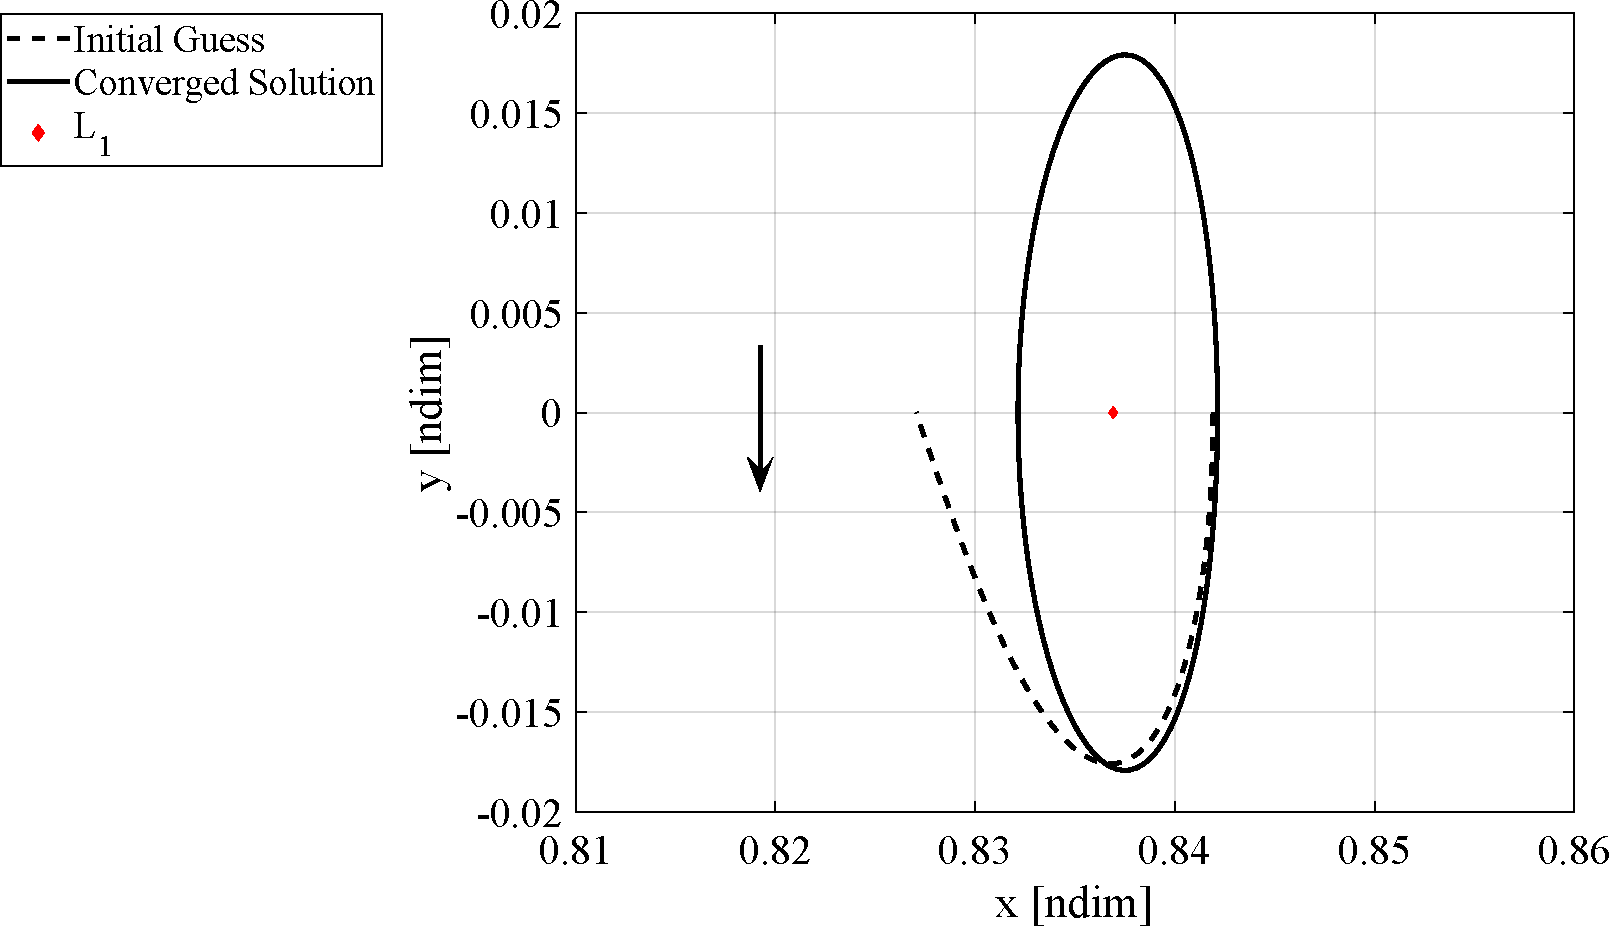
\includegraphics[width=0.75\textwidth]{figures/Lyapunov.pdf}
    \caption{Converged periodic Lyapunov orbit in the Earth-Moon barycentric rotating frame.}
    \label{fig:Lyapunov}
\end{figure}

\subsubsection{Natural Parameter Continuation}
The process described above produces a single solution near the Lagrange point. To compute more
solutions (orbits) in the family, especially further away from the Lagrange point where the linear
variational equations no longer apply, converged solutions can be used in a continuation scheme to
find other family members. This investigation utilizes natural parameter continuation, where one of
the parameters of a converged solution is changed by a small amount. This new guess for an orbit is
then converged, and a new solution is obtained. This continuation process can then be repeated
until the scheme reaches a natural/dynamical end or a desired orbit is reached. Natural parameters
of the orbit include (but are not limited to) components of the initial state, the period, or the
Jacobi constant. \cref{fig:L1Lyapunov} shows a large portion of the $L_{1}$ Lyapunov family in the
Earth-Moon system, continued in Jacobi constant from the orbit in \cref{fig:Lyapunov}. Lyapunov
families also exist about $L_{2}$ and $L_{3}$ and can be computed via the same process. Since
$L_{2}$ Lyapunovs are also used in this investigation, they are shown in \cref{fig:L2Lyapunov}.

\begin{figure}[ht]
    \centering
    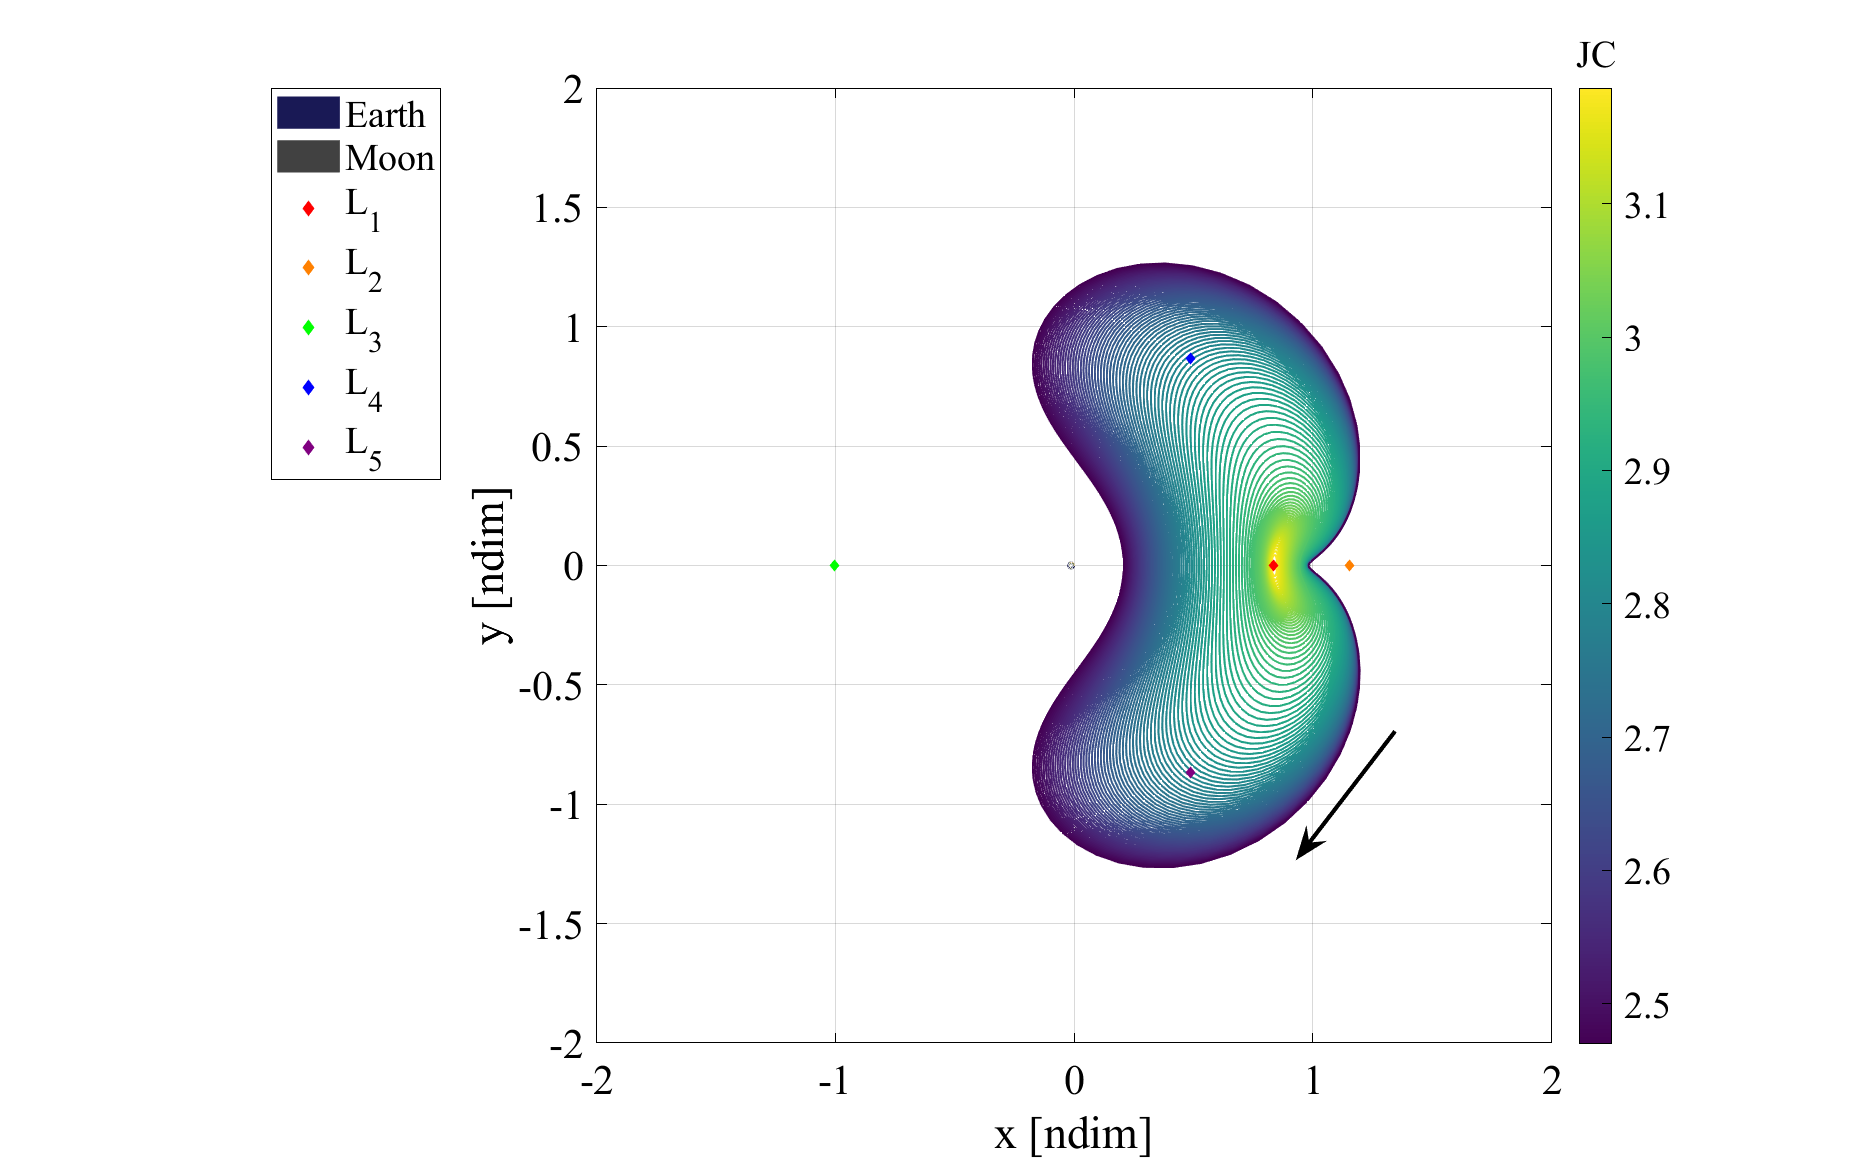
\includegraphics[width=0.9\textwidth]{figures/L1LyapunovFamily.pdf}
    \caption{Earth-Moon $L_{1}$ Lyapunov orbit family.}
    \label{fig:L1Lyapunov}
\end{figure}

\begin{figure}[ht]
    \centering
    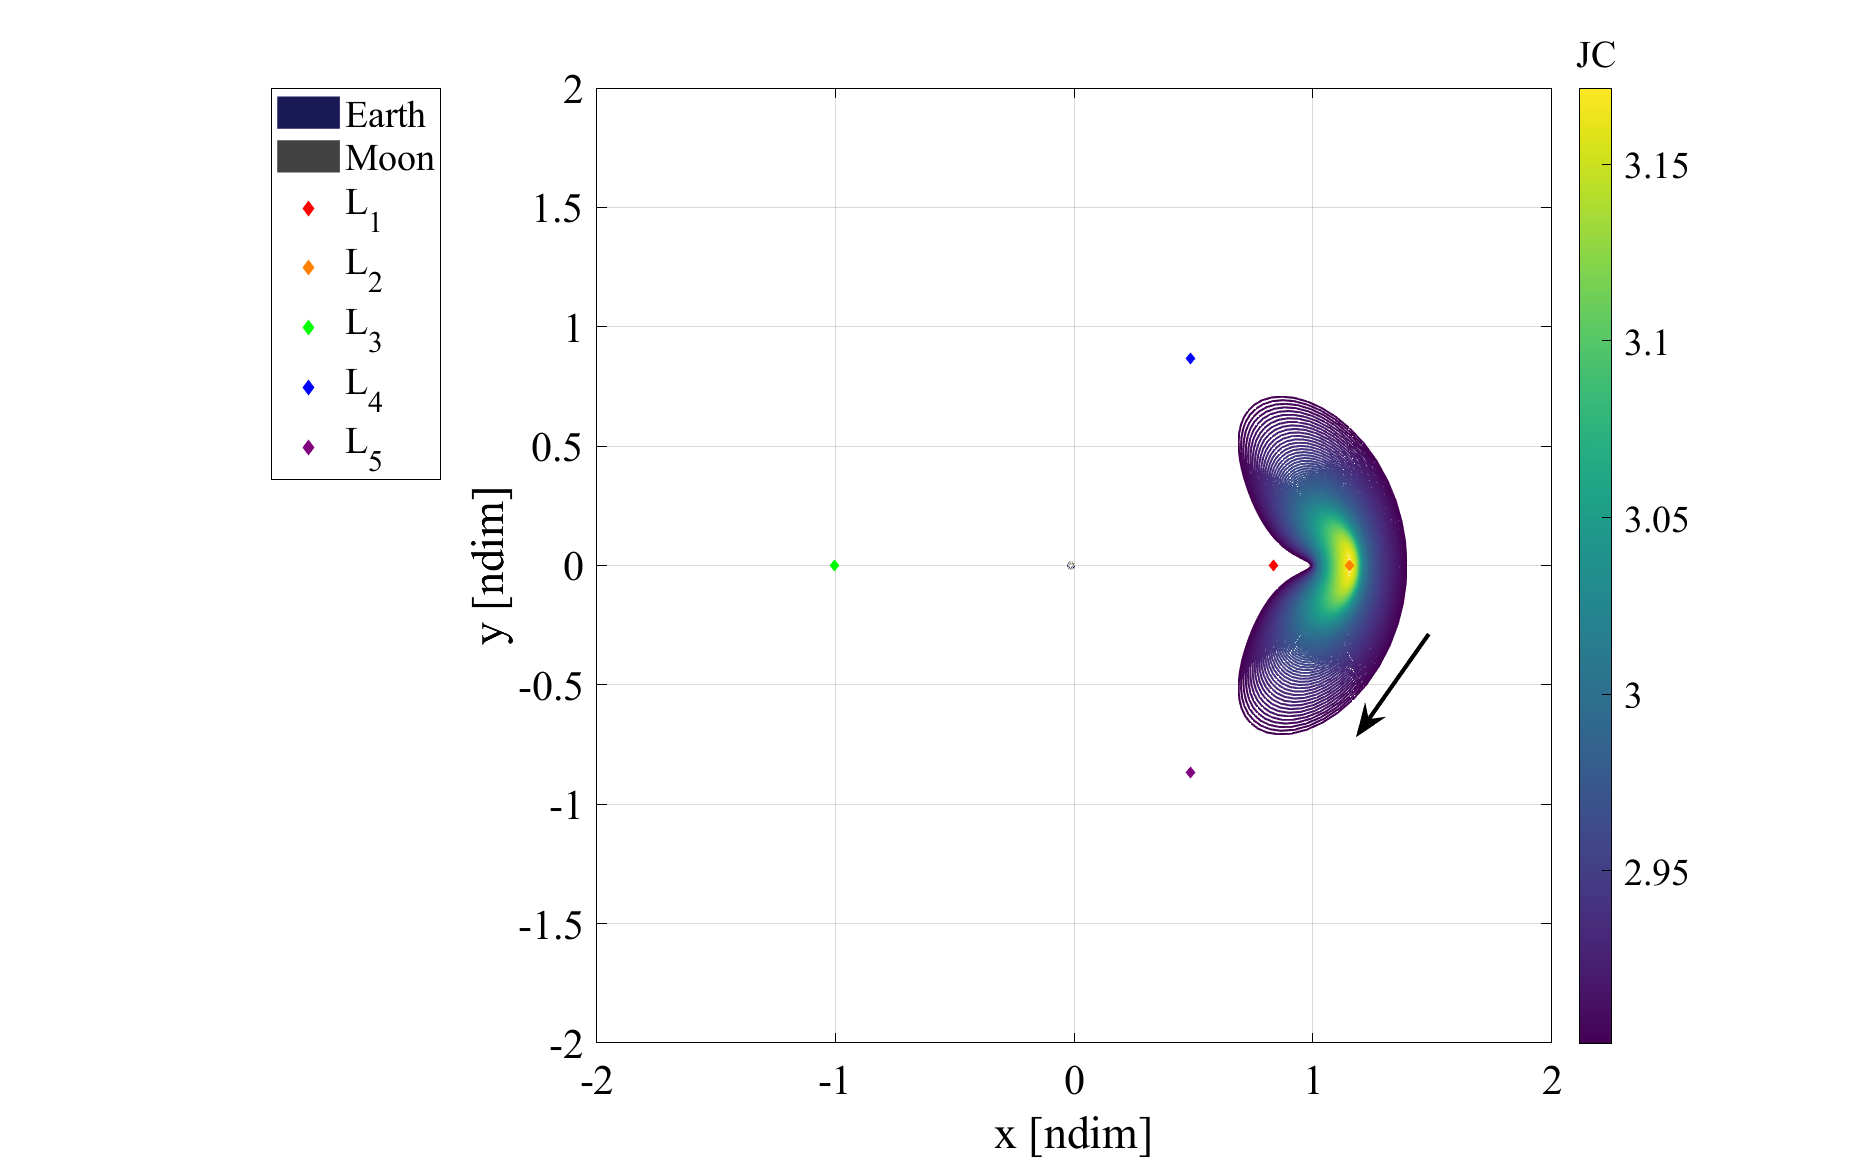
\includegraphics[width=0.9\textwidth]{figures/L2LyapunovFamily.pdf}
    \caption{Earth-Moon $L_{2}$ Lyapunov orbit family.}
    \label{fig:L2Lyapunov}
\end{figure}

\subsection{Orbital Stability}
Before discussing other orbit families, it is important to introduce orbital stability as it leads
to orbit family bifurcations and another way to generate new orbit families. Orbital stability
helps describe the characteristics of the orbit and the surrounding dynamics. The stability of an
orbit also determines the best transfer design strategies to minimize the $\Delta v$ cost. 

\phantomsection
\subsubsection{Monodromy Matrix}
The STM of one revolution of a periodic orbit in the CR3BP, $\Phi(t_{0}+\mathbb{P},t_{0})$, is
called the monodromy matrix, and discretely maps the linear growth of perturbations. Some
useful properties of the monodromy matrix are that it is symplectic, it has a determinant of $1$,
and its eigenvalues occur in reciprocal pairs\cite{ZimovanSpreen:2021}. Since the trajectory is
periodic, two of the eigenvalues (one pair) are always $1$, denoted the trivial pair, and
correspond to the trajectory's periodicity and membership in a family of solutions.

The stability of the orbit is characterized by the remaining two pairs of eigenvalues. Since the
monodromy matrix is a discrete-time mapping, eigenvalues that lie within the unit circle (magnitude
less than $1$) in the complex plane are stable and those outside the unit circle are unstable.
Perturbations in the stable subspace will flow back toward the orbit, while perturbations in the
unstable subspace will depart the orbit. If the eigenvalues lie directly on the unit circle, then
the corresponding flow is in the center subspace and remains bounded around the orbit. When the
stability of an eigenvalue pair changes, it can indicate a change in the characteristics of orbits
within a family and sometimes leads to a bifurcation in the family, discussed later.

The overall stability of the orbit is then determined by all of the eigenvalues of its monodromy
matrix. If any of the eigenvalues are unstable (greater than $1$), then the orbit is considered
linearly unstable. Note that the existence of an unstable eigenvalue implies the existence of a
stable eigenvalue because of the reciprocal pairs. Otherwise, the orbit is considered marginally
stable and all of the eigenvalues reside on the unit circle. Throughout an orbit family, while the
stability of the members may change, the eigenvalues experience a smooth (but not necessarily
monotonic) evolution.

\subsubsection{Stability Index}
A variety of metrics exist to more succinctly portray the stability of orbits, rather than viewing
all of the eigenvalues. One such metric is a stability index, of which there are a variety of
definitions whose usefulness vary depending on the application. In this investigation, the focus is
on just the overall stability of the orbit --- whether it is unstable or marginally stable --- so a
metric that can quickly differentiate between these behaviors suffices. Therefore, the following
definition is used\cite{Power:2019}:
\begin{equation}
    \varsigma=||\bar{\lambda}||_{\inf},
    \label{eq:stabilityindex}
\end{equation}
where $\bar{\lambda}$ is a vector of the eigenvalues of the monodromy matrix and the infinity norm
returns the magnitude of the largest (magnitude) element of the vector. With this definition,
$\varsigma>1$ indicates an unstable orbit and $\varsigma=1$ indicates one that is marginally
stable. Other definitions can be found in Zimovan Spreen's work\cite{ZimovanSpreen:2021}.

Like the eigenvalues themselves, the evolution of the stability index over an orbit family is
smooth. \cref{fig:stability} shows the stability indices for the members of the $L_{1}$ (a) and
$L_{2}$ (b) Lyapunov families from \cref{fig:L1Lyapunov} and \cref{fig:L2Lyapunov}. A larger
stability index means that the orbit has a higher instability and perturbations will experience
faster growth. Note that all of the members of both of these families are unstable. However, there
are stability changes among individual eigenvalues within each family that can lead to
bifurcations.

\begin{figure}[ht]
    \begin{subfigure}[h]{0.4\linewidth}
        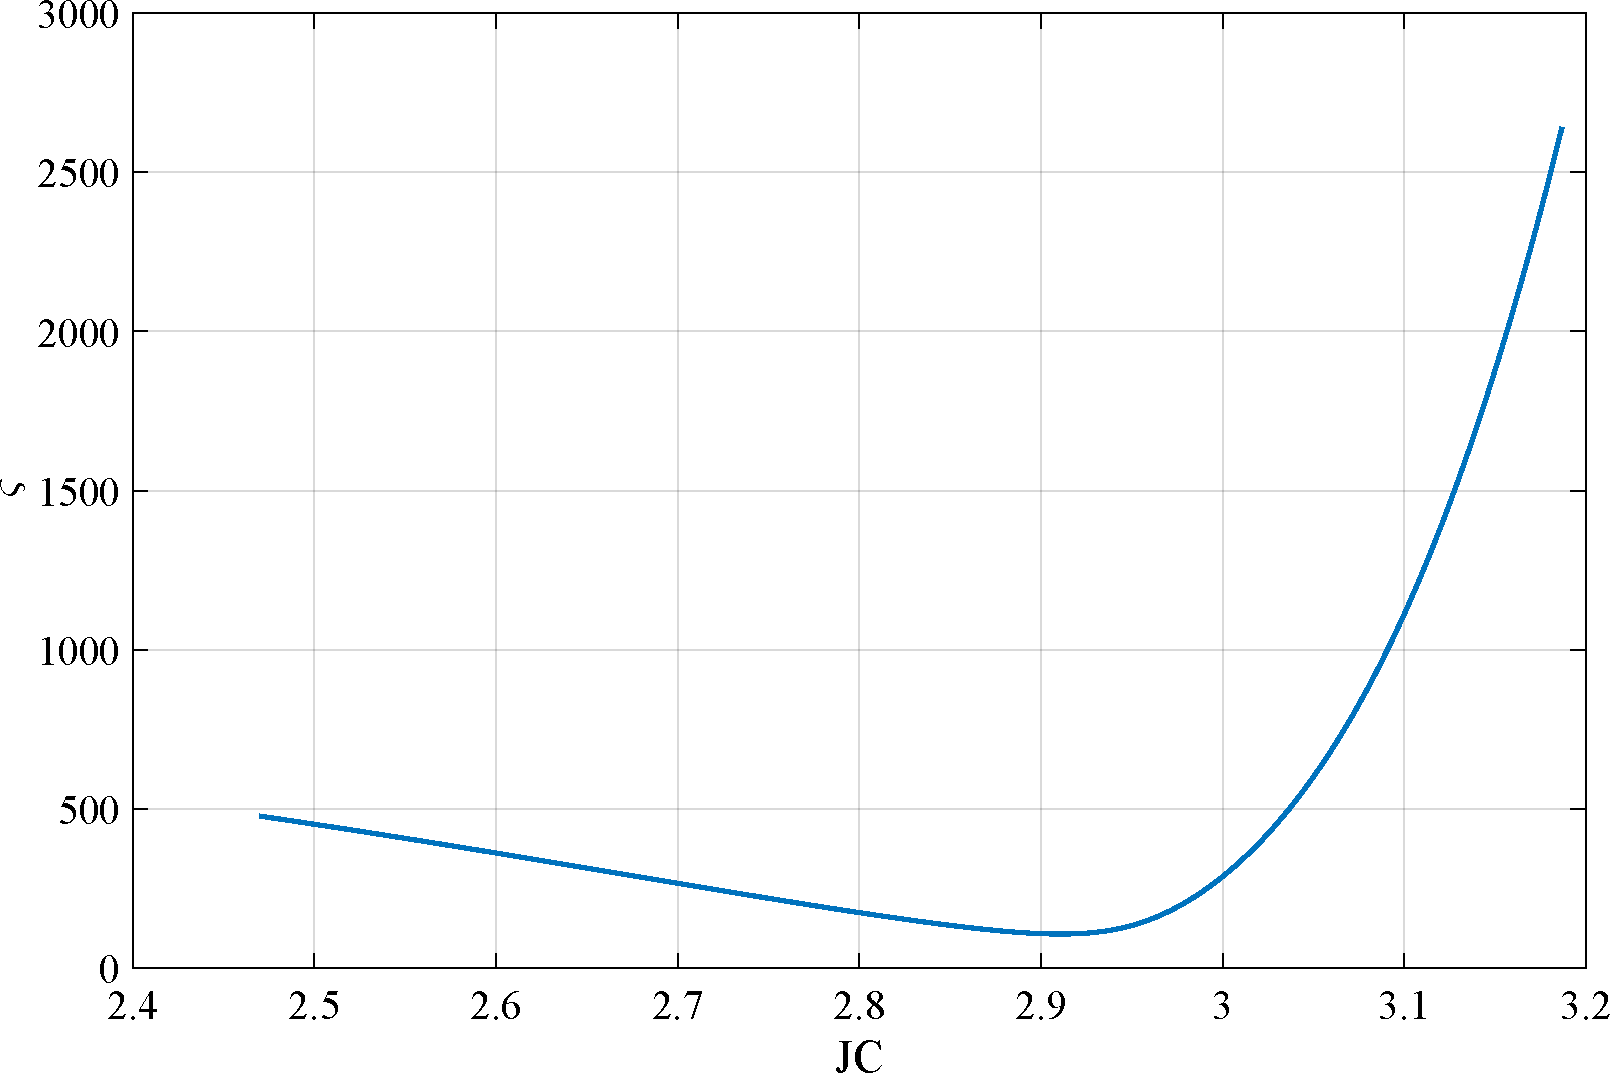
\includegraphics[width=\textwidth]{figures/L1LyapunovStability.pdf}
        \caption{$L_{1}$}
    \end{subfigure}
    \hfill
    \begin{subfigure}[h]{0.4\linewidth}
        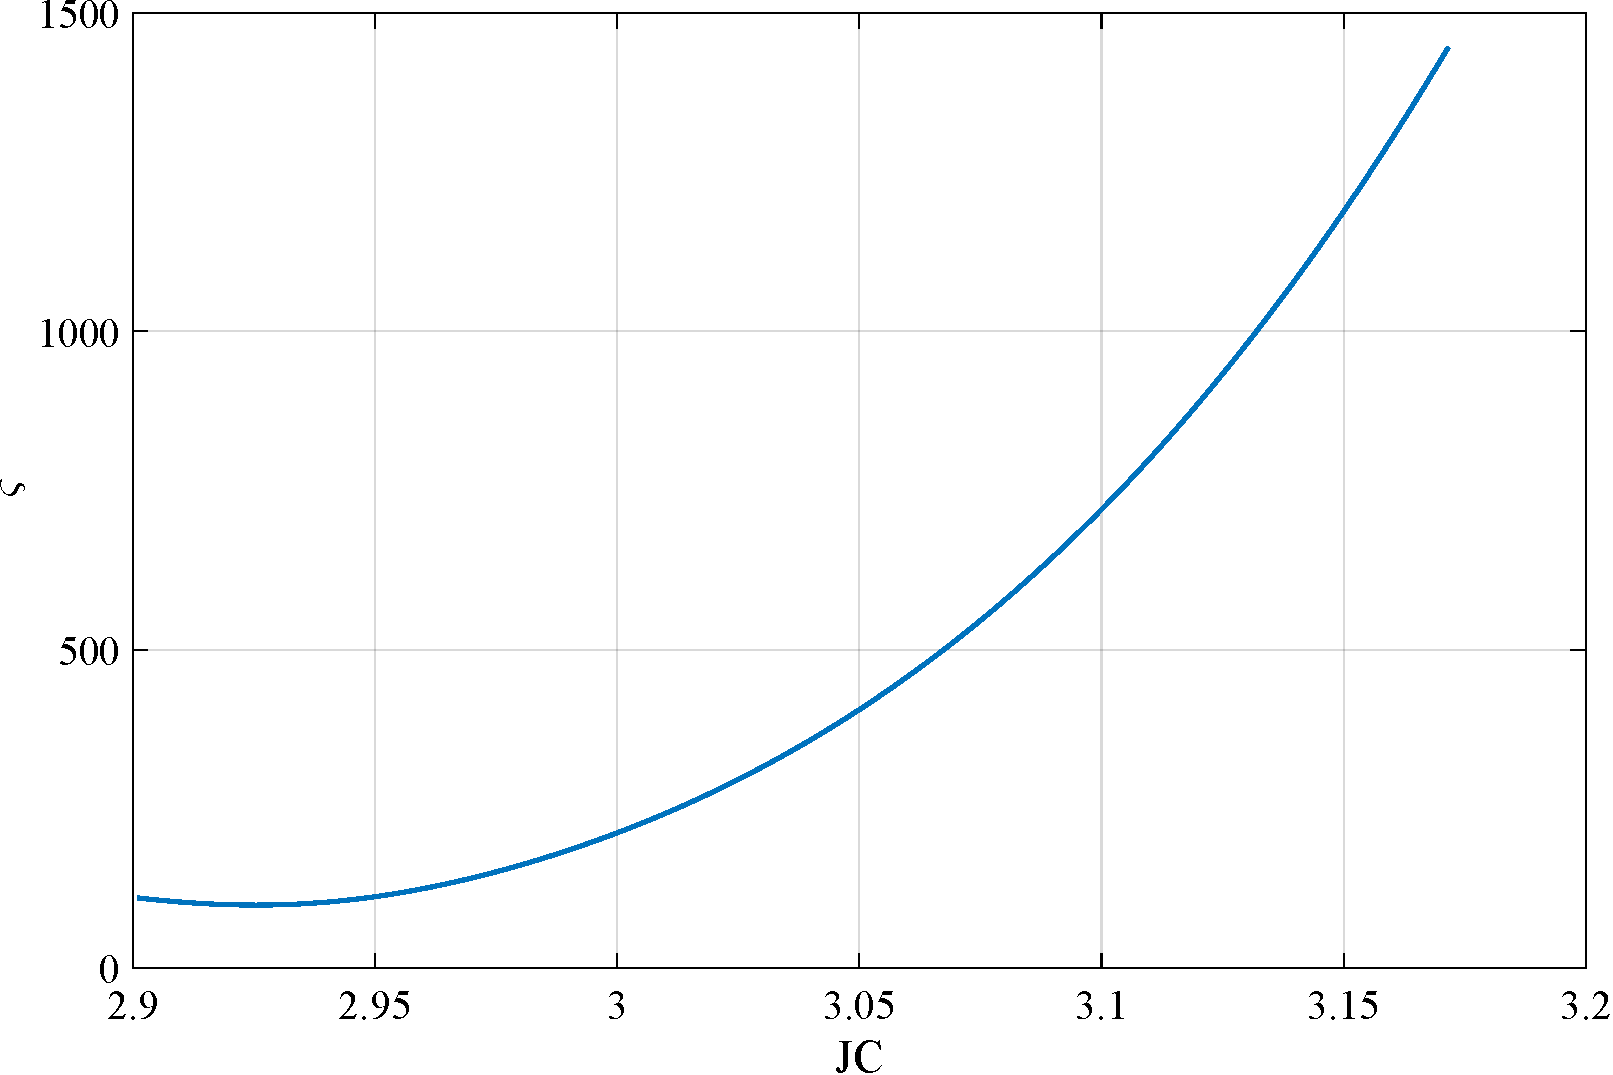
\includegraphics[width=\textwidth]{figures/L2LyapunovStability.pdf}
        \caption{$L_{2}$}
    \end{subfigure}
    \caption{Earth-Moon Lyapunov family stability index evolution.}
    \label{fig:stability}
\end{figure}

\subsubsection{Time Constant}
Another useful metric of stability is the time constant, which approximates how long it takes, in
time units or in orbit revolutions, for a perturbation to grow by a factor of $e$:
\begin{equation}
    \Upsilon=\frac{1}{\ln\varsigma},
    \label{eq:timeconstant}
\end{equation}
where the dimensions are orbit revolutions. This equation can be multiplied by the period of the
orbit $\mathbb{P}$ to produce the time constant in time units. \cref{fig:timeConstant} shows the
time constant evolution of both Lyapunov families in orbit revolutions. Note that a larger time
constant indicates that it takes longer for a perturbation, meaning that the orbit is less
unstable, and a marginally stable orbit has an infinite time constant.

\begin{figure}[ht]
    \begin{subfigure}[h]{0.4\linewidth}
        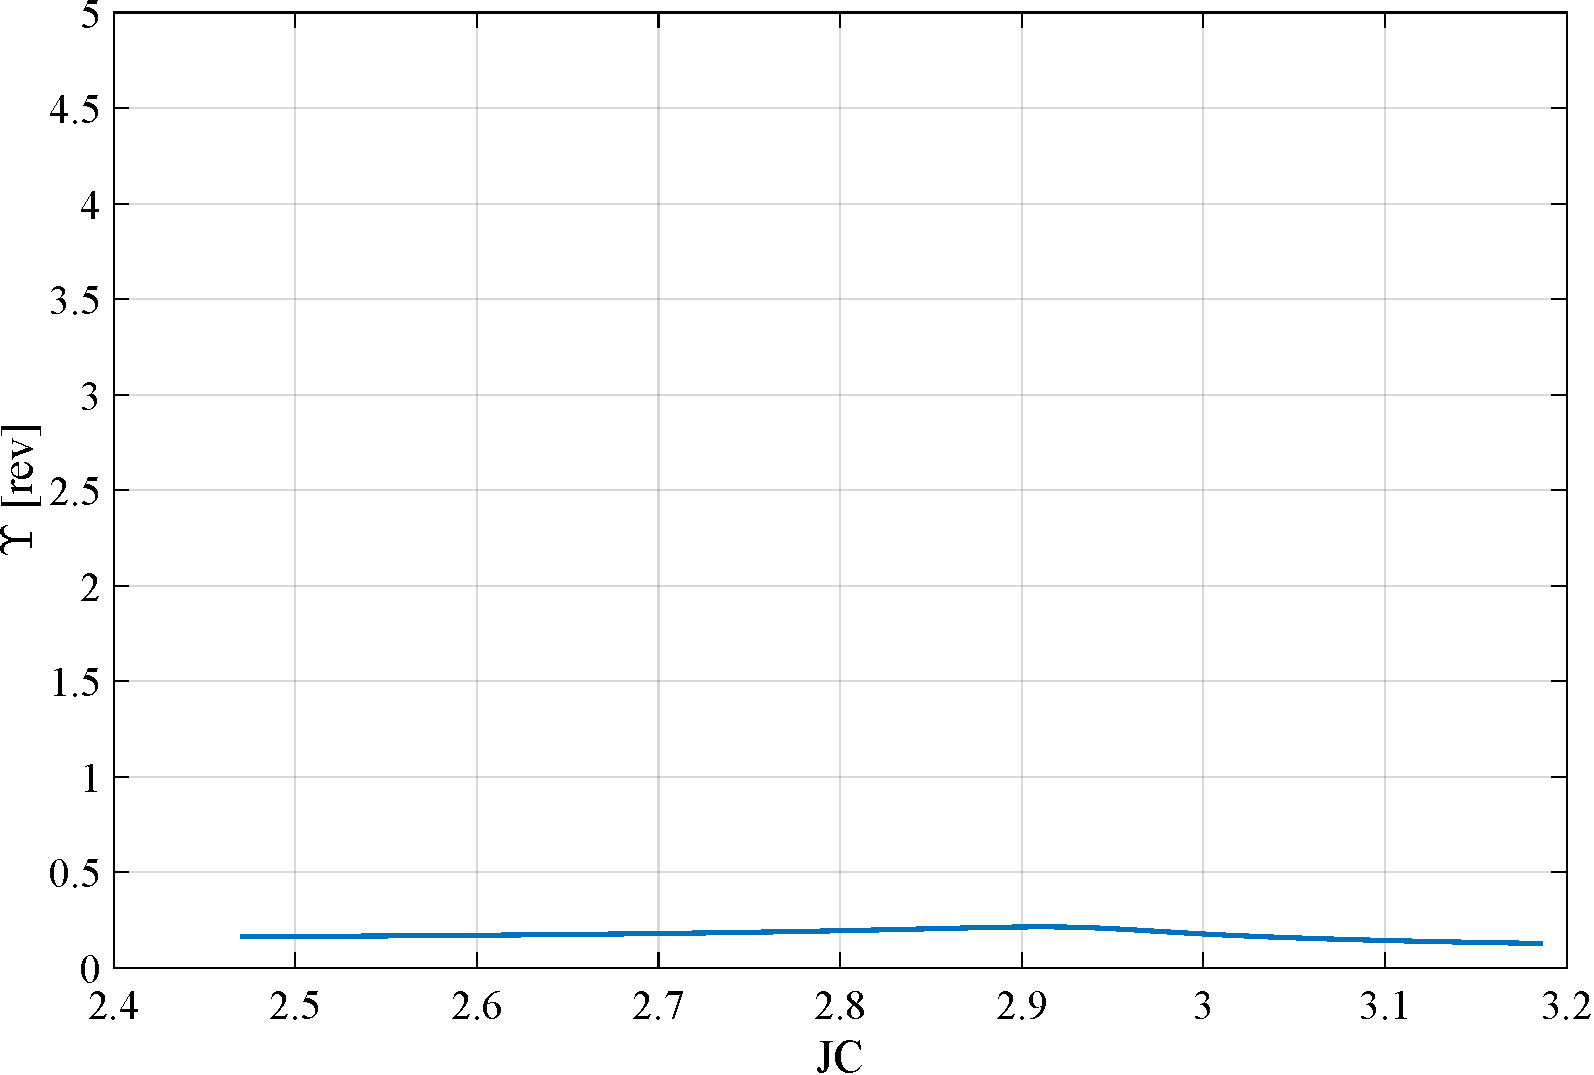
\includegraphics[width=\textwidth]{figures/L1LyapunovTimeConstant.pdf}
        \caption{$L_{1}$}
    \end{subfigure}
    \hfill
    \begin{subfigure}[h]{0.4\linewidth}
        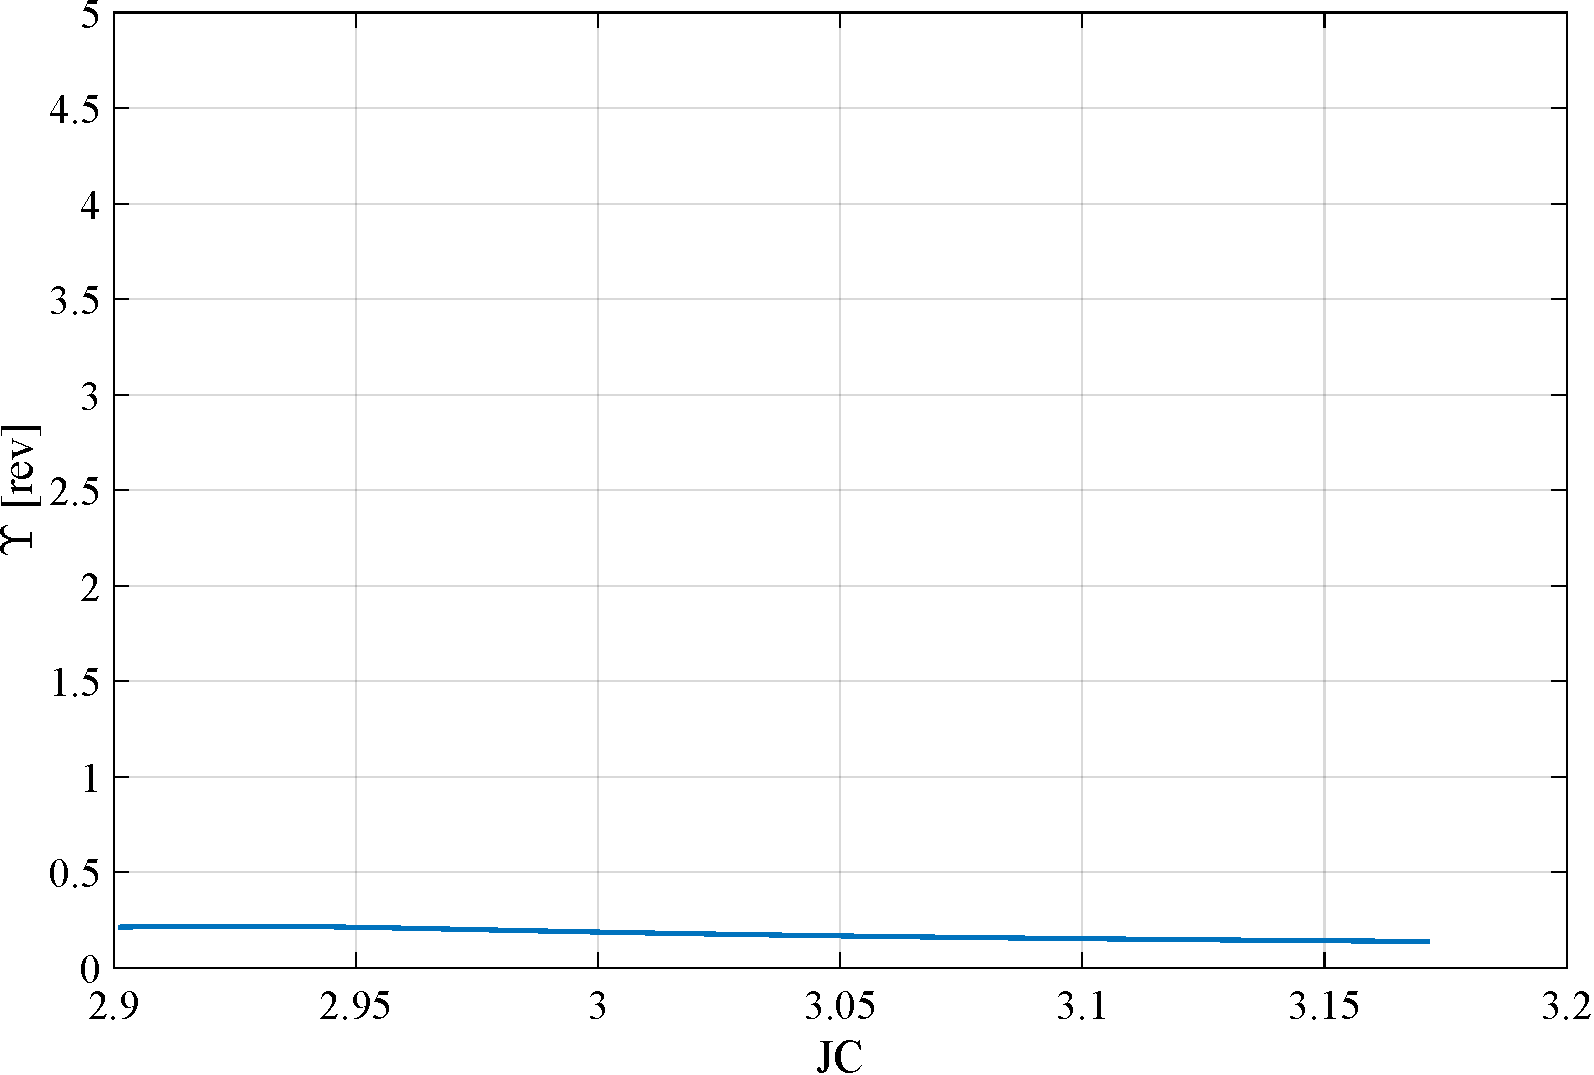
\includegraphics[width=\textwidth]{figures/L2LyapunovTimeConstant.pdf}
        \caption{$L_{2}$}
    \end{subfigure}
    \caption{Earth-Moon Lyapunov family time constant evolution.}
    \label{fig:timeConstant}
\end{figure}

\subsubsection{Bifucations}
Within the context of the CR3BP, bifurcation theory can be used to detect changes in orbit
stability characteristics within a family that can sometimes lead to the generation of orbit
families that branch off from the original family. Zimovan Spreen provides a more thorough
analysis of how bifurcation theory can be applied to the CR3BP so only the information most
relevant to this investigation will be provided here\cite{ZimovanSpreen:2021}.

Two main bifurcation types are relevant to the orbits used in this analysis:
\begin{itemize}
    \item \textbf{Tangent bifurcations} occur when an eigenvalue pair goes to $1$, either from the
    unit circle or the real axis. With a cyclic fold tangent bifurcation, which occurs at an
    extremum in the Jacobi constant, the stability of the eigenvalues changes, but there is no new
    family of solutions created. Pitchfork tangent bifurcations produce two new families that have
    the same stability as the original family. The last subtype, transcritical tangent
    bifurcations, produce a new family and a change in the eigenvalue stability of the original
    family.
    \item \textbf{Period-multiplying bifurcations} occur when an eigenvalue pair reaches a root of
    $1$ ($\sqrt{1}$, $\sqrt[3]{1}$, $\sqrt[m]{1}$, etc.). In general, this produces a new family
    with a period of $m$ times the original, but not necessarily a change in stability. The most
    commonly seen subtype is the period-doubling bifurcation, where the pair of eigenvalues meets
    at $-1$, either from the unit circle or the real axis. This results in a change in the
    stability of the eigenvalues and a new family that has double the period of the original
    family.
\end{itemize}
There are other methods of detecting bifurcations beyond examining the evolution of the eigenvalues
such as Broucke stability or bifurcation diagrams that are also described in Zimovan
Spreen\cite{ZimovanSpreen:2021}.

\subsubsection{New Family Generation from Bifurcation}
To find the initial conditions for an orbit in a new family from a bifurcation, first, the precise
bifurcating orbit (within a tolerance) must be obtained. This can be done through a simple
bisection algorithm. The Jacobian matrix of this bifurcating orbit should have an additional
nullspace compared to the other orbits in the family since another pair of eigenvalues (besides the
trivial pair) is at $1$. Note that for a period-multiplying bifurcation, the orbit must be
propagated for $m$ revolutions to obtain the proper Jacobian matrix. When this is the case, one of
the nullspace vectors points in the direction of continuing the old family, while the other vector
indicates a direction for the new family.

Using a singular value decomposition (SVD), this new nullspace direction can be identified by the
right singular vector of $DF$ that corresponds to the additional nullspace. Stepping in this
direction from the bifurcating orbit's initial conditions and correcting for a periodic solution
should result in a new periodic orbit belonging to the new family. This approach is also known as
pseudo-arclength continuation and the new member can then be continued using any scheme to obtain
the new family.

\subsection{Halo Orbits}
\phantomsection
\subsubsection{A Halo Targeter}
Similar to Lyapunov orbits, halo orbits are symmetric about the $xz$-plane although they are
spatial in the rotating frame and not limited to the $xy$-plane. This again allows for
targeting only half of the periodic orbit, from one perpendicular crossing to the next. Since there
is now a $z$-component to the orbits, it is helpful to introduce a new free variable and constraint
for the halo targeter:
\begin{equation}
    \Xbar=\begin{bmatrix}   x_{0}   &   z_{0}   &   \ydot_{0}   &   \tau    \end{bmatrix}^{T},
    \label{eq:halofreevar}
\end{equation}
\begin{equation}
    \Fbar(\Xbar)=\begin{bmatrix}    y_{f}   &   \xdot_{f}   &   \zdot_{f}   &   C-C_{d} \end{bmatrix}^{T}=\zerobar,
    \label{eq:haloconst}
\end{equation}
\begin{equation}
    DF(\Xbar)=\begin{bmatrix}   \phi_{21}                                                                   &   \phi_{23}                                               &   \phi_{25}                                   &   \ydot_{f}                               \\
                                \phi_{41}                                                                   &   \phi_{43}                                               &   \phi_{45}                                   &   \xddot_{f}                              \\
                                \phi_{61}                                                                   &   \phi_{63}                                               &   \phi_{65}                                   &   \zddot_{f}                              \\
                                2x_{0}-\frac{2(x_{0}+\mu)(1-\mu)}{d^{3}}-\frac{2\mu(x_{0}-1+\mu)}{r^{3}}    &   -\frac{2z_{0}(1-\mu)}{d^{3}}-\frac{2z_{0}\mu}{r^{3}}    &   -2\ydot_{0}                                 &   0                                       \end{bmatrix}.
    \label{eq:halojacobian}
\end{equation}
The result of this targeting will provide the initial state ($y_{0}=\xdot_{0}=\zdot_{0}=0$) and
half of the propagation time for a periodic halo orbit.

\subsubsection{Converged Halo Families}
The initial guess for a halo orbit comes from a bifurcating orbit in a Lyapunov family. At
$C\approx3.174352$, the $L_{1}$ Lyapunov family has a tangent bifurcation and the $L_{1}$ halo
family is formed. The pseudo-arclength method for generating an initial guess can be used as
described above to obtain the initial guess for the initial state, propagation time, and Jacobi
constant. Using natural parameter continuation, more of the family is produced, shown in
\cref{fig:L1Halo}. Since the Lyapunov orbit can bifurcate above or below the $xy$-plane, two halves
of the family are formed. \cref{fig:L1Halo} is denoted the $L_{1}$ southern halos because most of
the orbit is spent south (in the rotating frame) of the Moon.

\begin{figure}[ht]
    \centering
    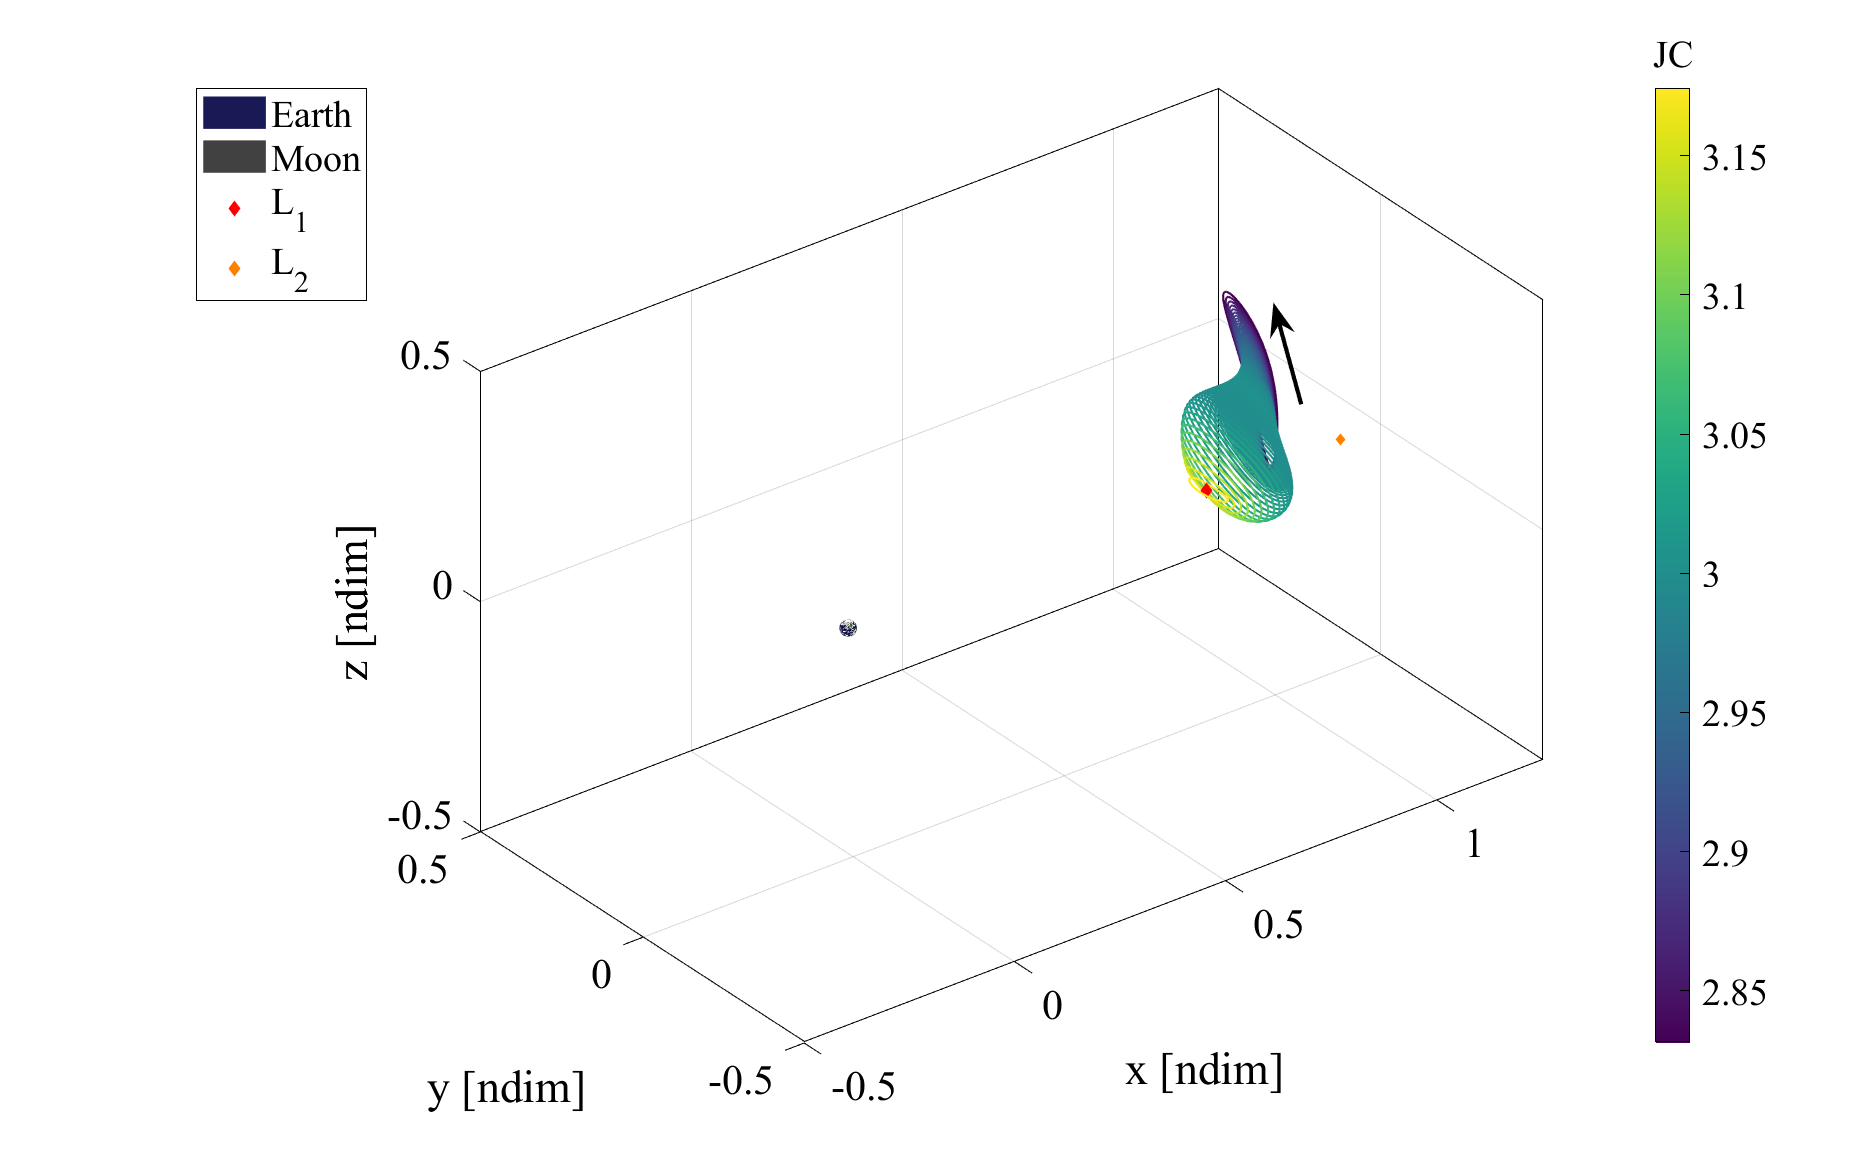
\includegraphics[width=0.9\textwidth]{figures/L1HaloFamily.pdf}
    \caption{Earth-Moon $L_{1}$ southern halo orbit family.}
    \label{fig:L1Halo}
\end{figure}

\cref{fig:L2Halo} shows the $L_{2}$ southern halo family, generated in the same way as the $L_{1}$
halos but from the $L_{2}$ Lyapunov family. Note that these halo families are not monotonic in
Jacobi constant. The stability indices for both families are shown in \cref{fig:haloStability}.
$L_{3}$ halos also exist, but are not used in this investigation.

\begin{figure}[ht]
    \centering
    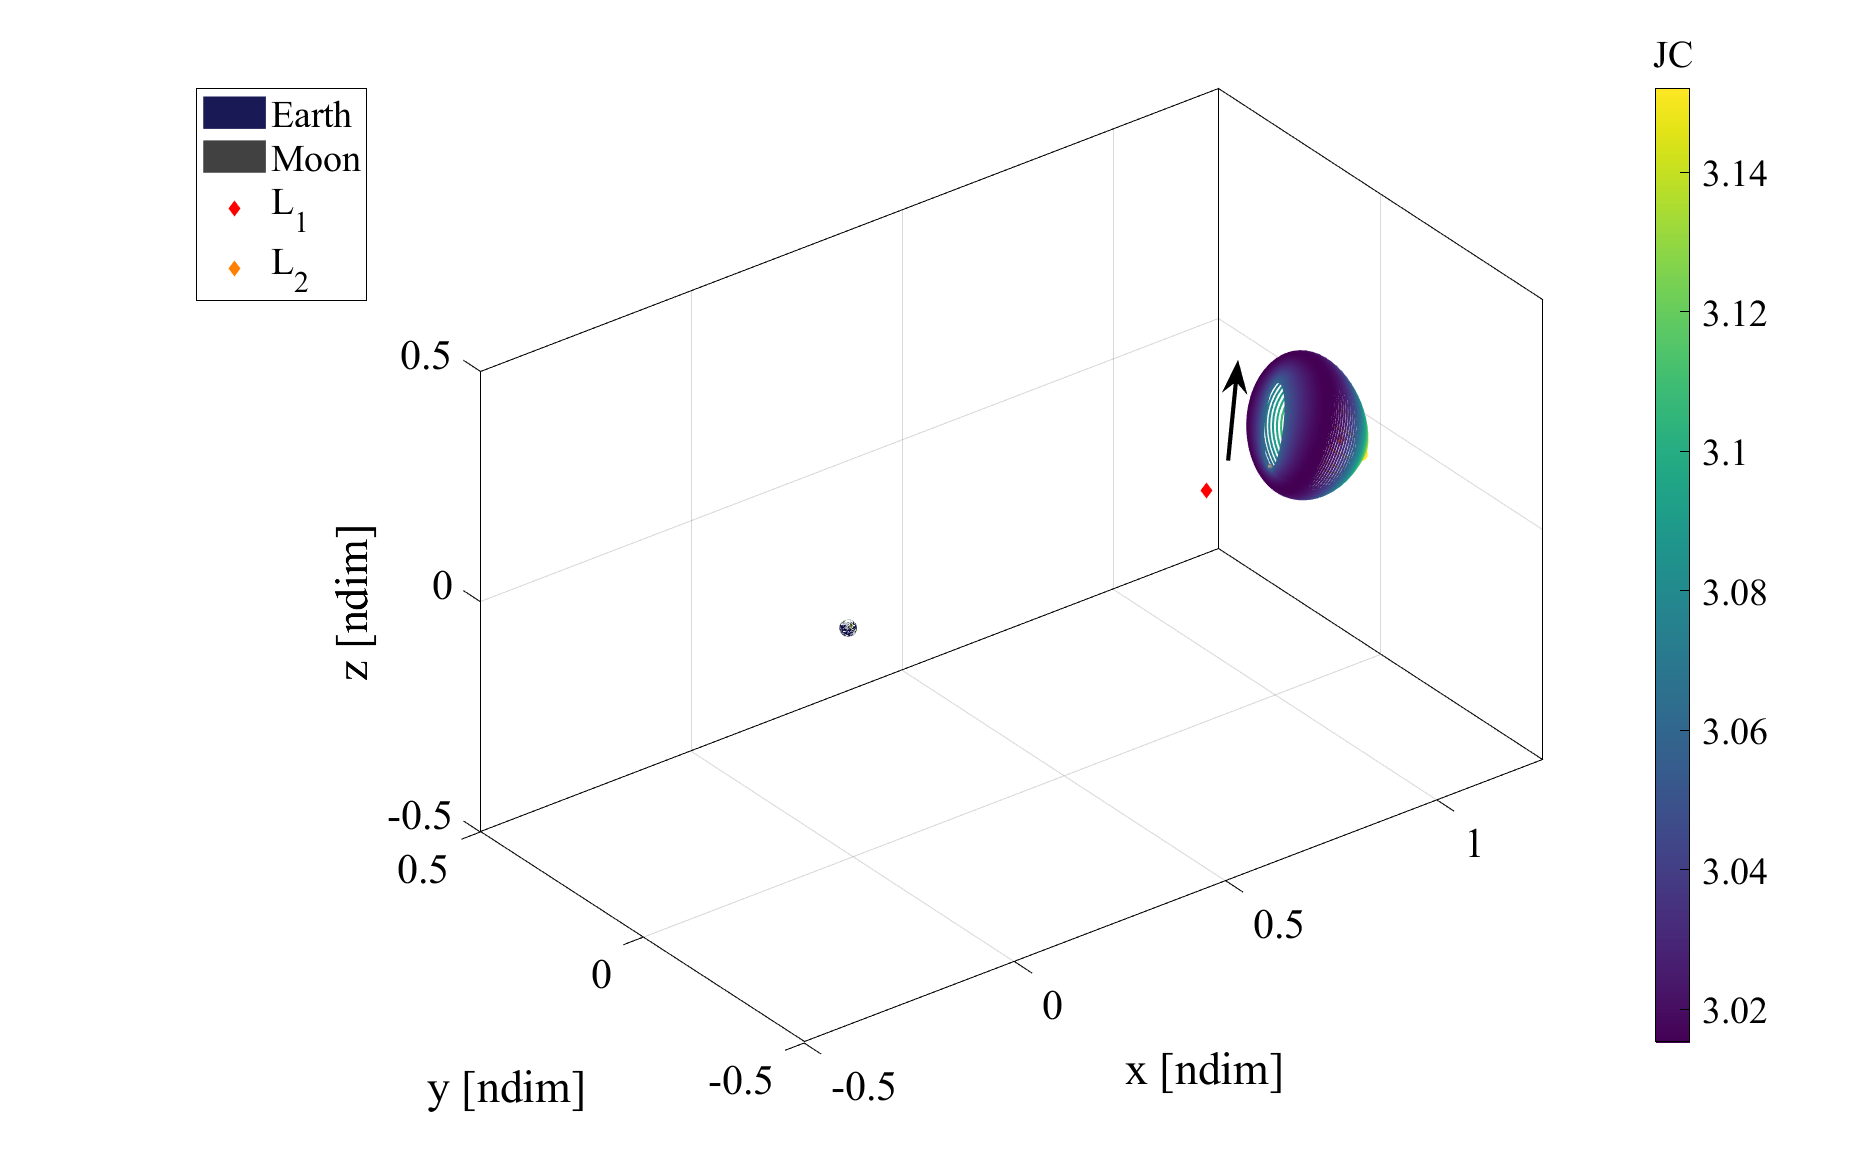
\includegraphics[width=0.9\textwidth]{figures/L2HaloFamily.pdf}
    \caption{Earth-Moon $L_{2}$ southern halo orbit family.}
    \label{fig:L2Halo}
\end{figure}

\begin{figure}[ht]
    \begin{subfigure}[h]{0.4\linewidth}
        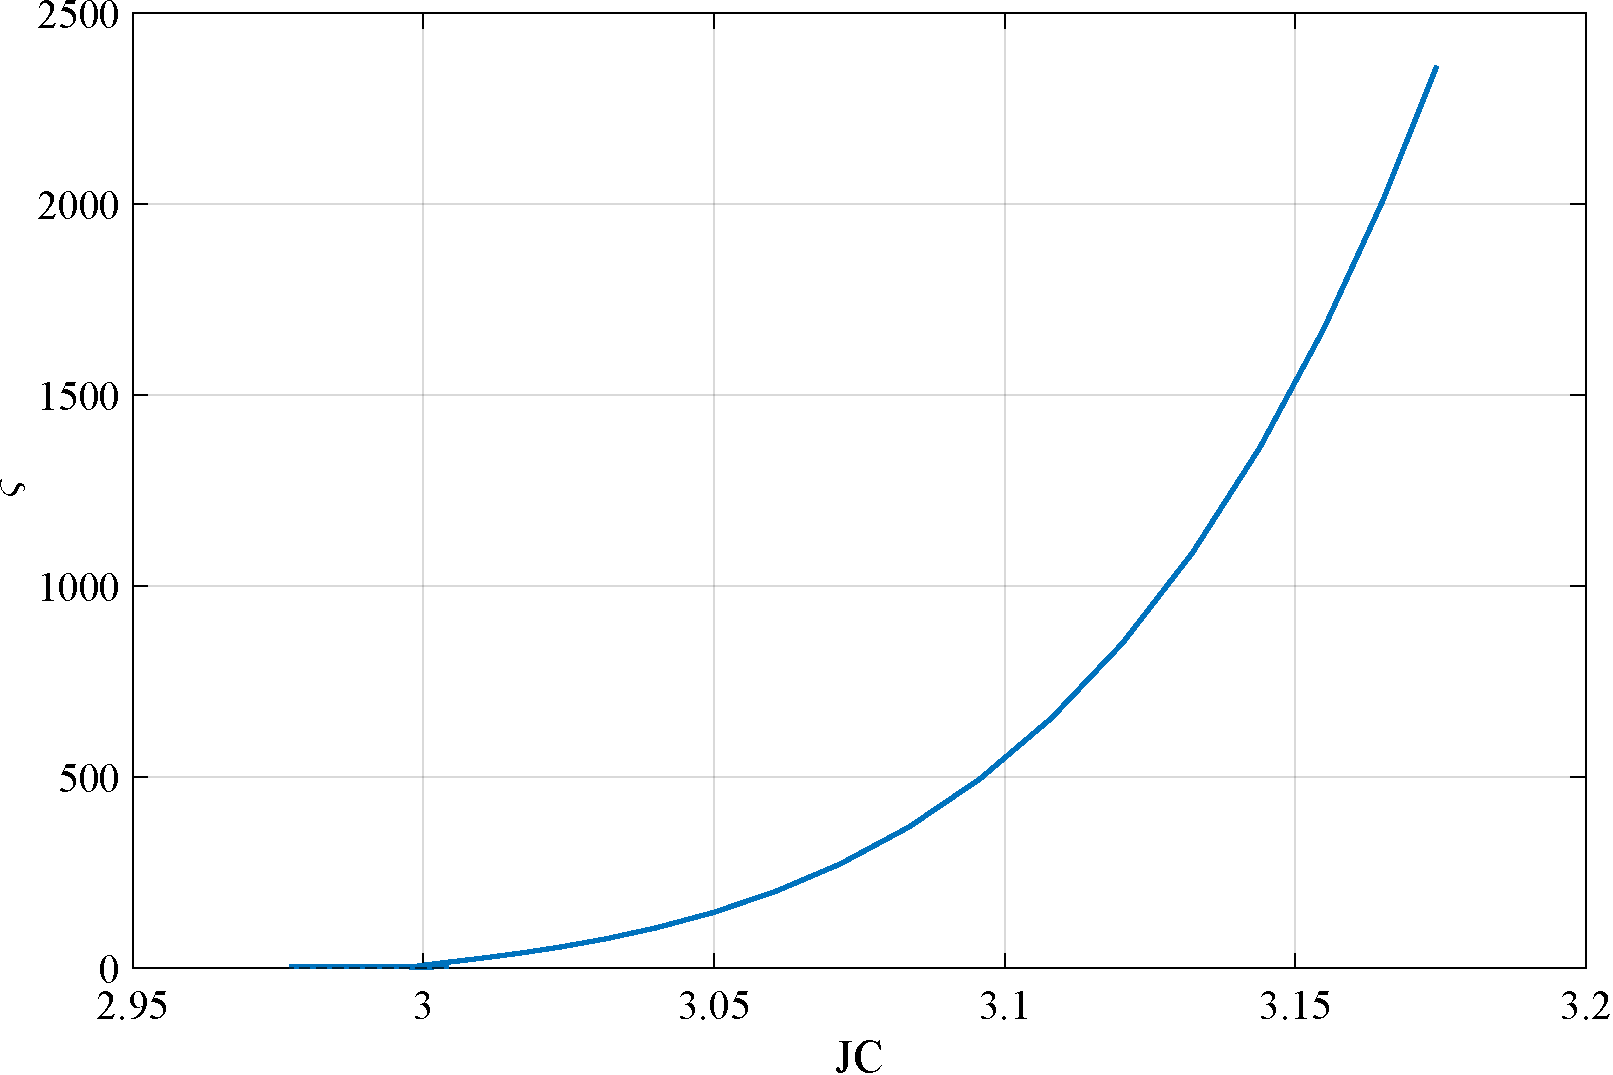
\includegraphics[width=\textwidth]{figures/L1HaloStability.pdf}
        \caption{$L_{1}$}
    \end{subfigure}
    \hfill
    \begin{subfigure}[h]{0.4\linewidth}
        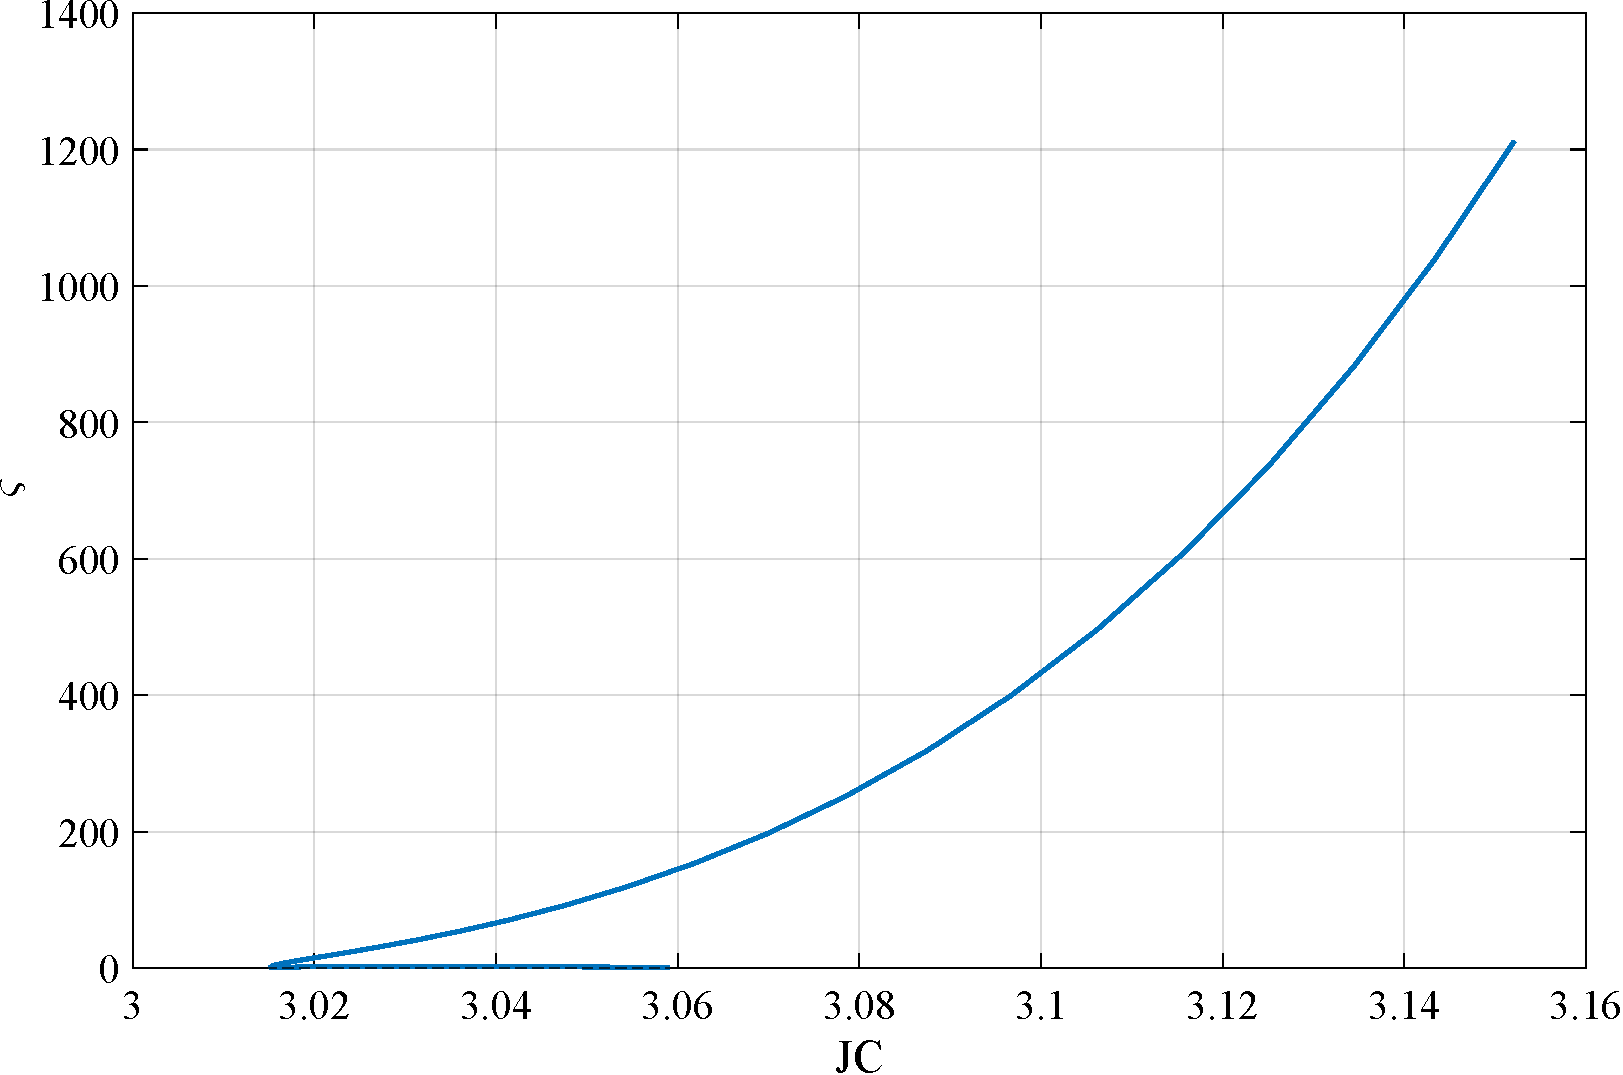
\includegraphics[width=\textwidth]{figures/L2HaloStability.pdf}
        \caption{$L_{2}$}
    \end{subfigure}
    \caption{Earth-Moon Halo family stability index evolution.}
    \label{fig:haloStability}
\end{figure}

\subsection{Butterfly Orbits}
Butterfly orbits is another name for the $P_{2}HO_{1}$ $L_{2}$ orbit family: the period-doubling
bifurcation from the $L_{2}$ halo family with the smallest perilune\cite{ZimovanSpreen:2021}.
Conveniently, the same targeter can be used for this family as with the halos above. The same
pseudo-arclength method can also be used to obtain the initial guess from the bifurcating halo,
remembering to double the period of the orbit first. A portion of this family is shown in
\cref{fig:butterfly} and the stability indices are shown in \cref{fig:butterflyStability}.

\begin{figure}[ht]
    \centering
    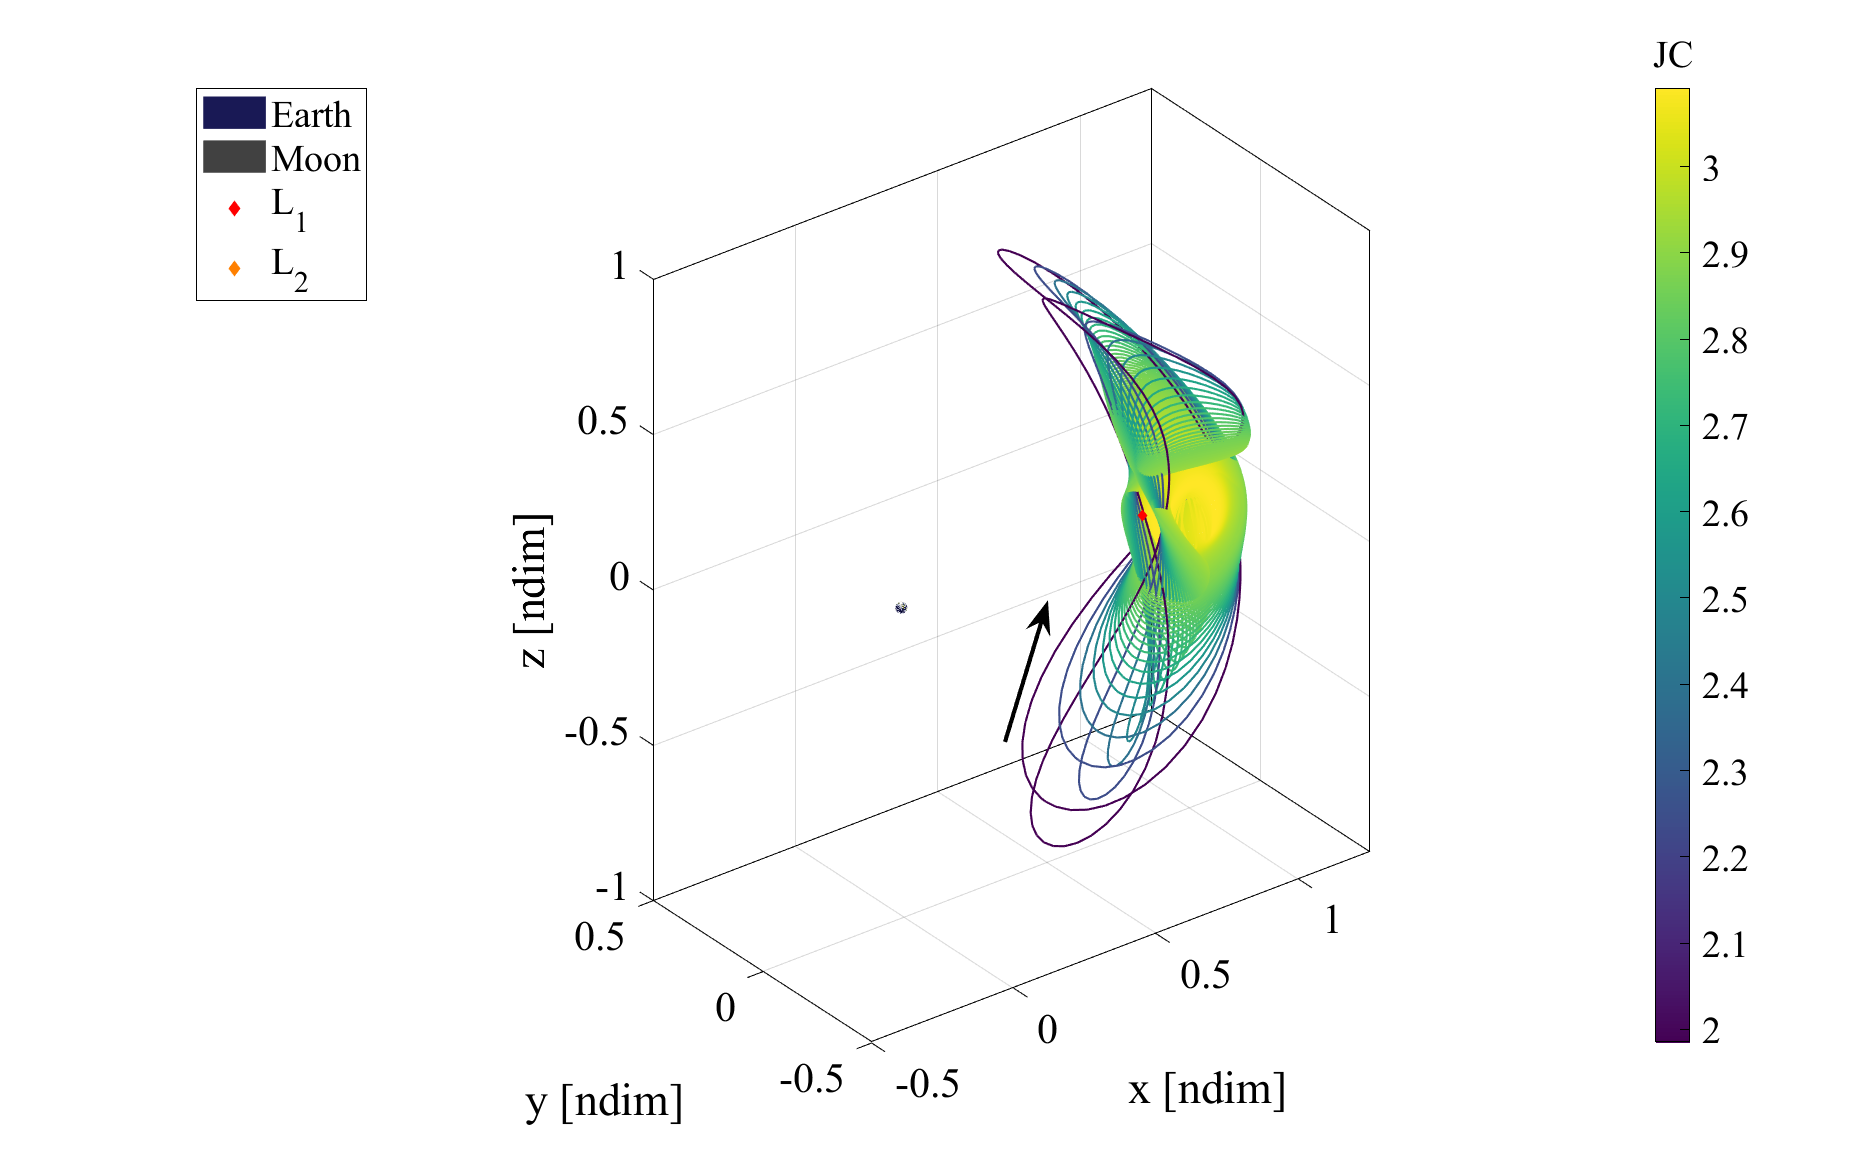
\includegraphics[width=0.9\textwidth]{figures/L2ButterflyFamily.pdf}
    \caption{Earth-Moon butterfly family.}
    \label{fig:butterfly}
\end{figure}

\begin{figure}[ht]
    \centering
    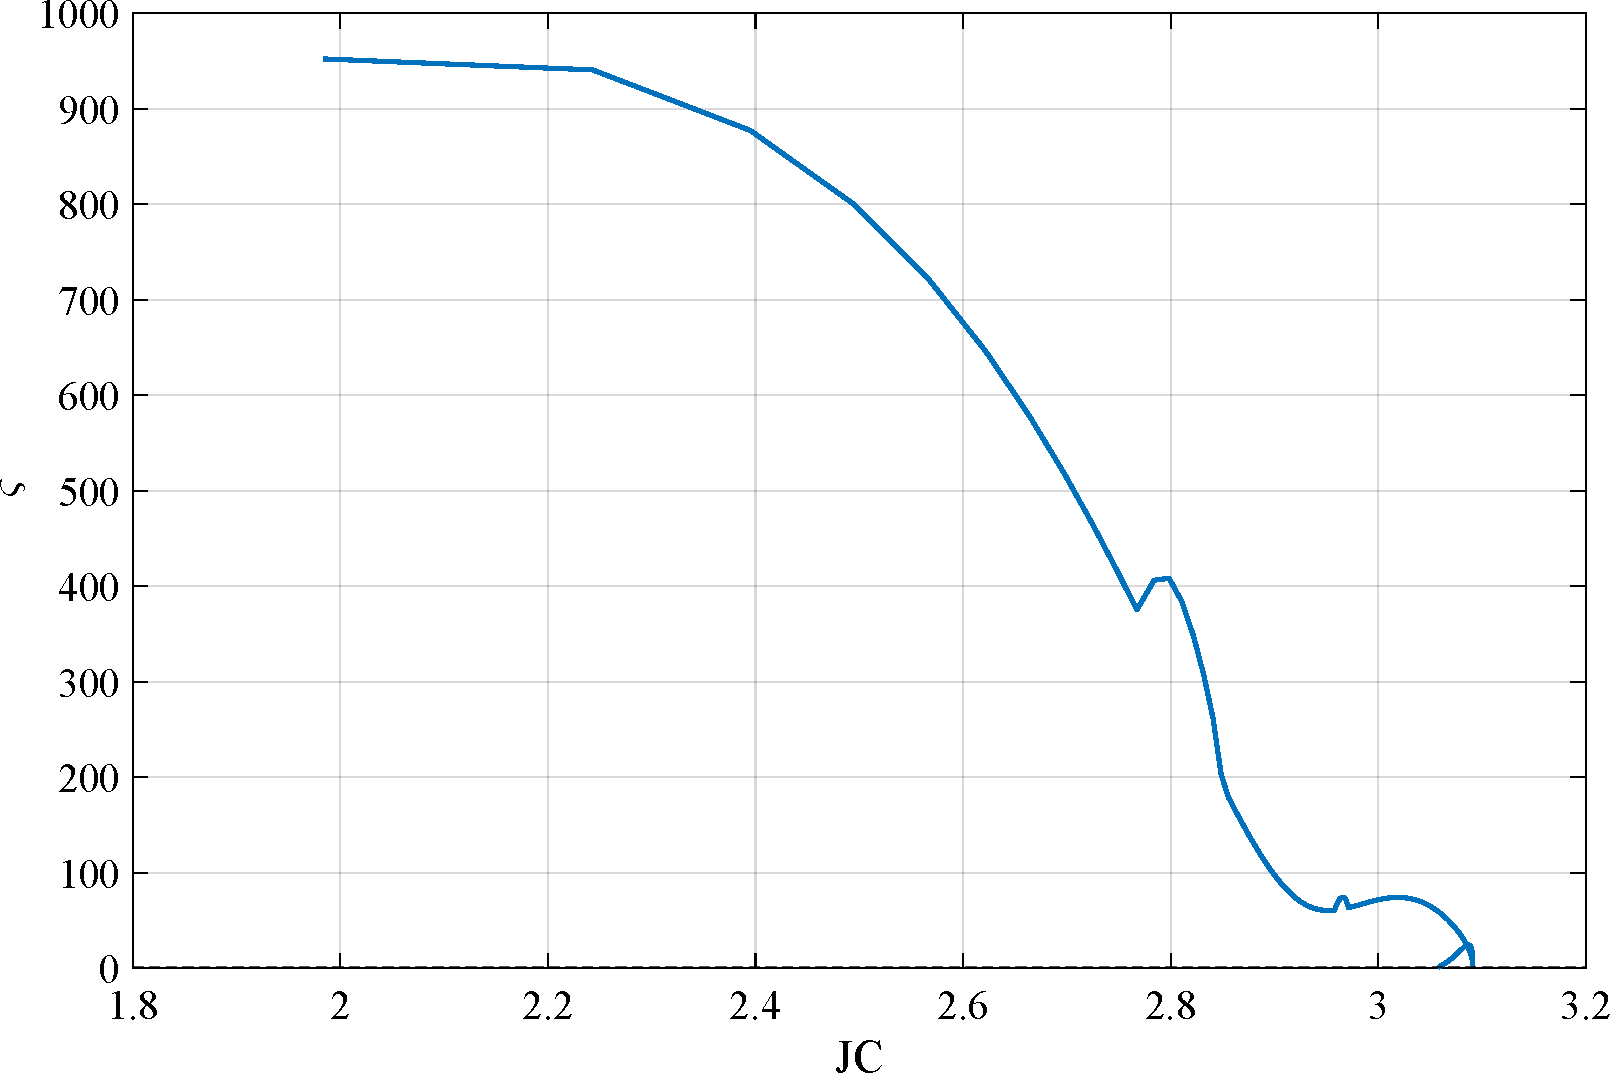
\includegraphics[width=0.5\textwidth]{figures/L2ButterflyStability.pdf}
    \caption{Earth-Moon butterfly family stability index evolution.}
    \label{fig:butterflyStability}
\end{figure}

\subsection{Axial Orbits}
\phantomsection
\subsubsection{An Axial Targeter}
Another spatial orbit family, the axial orbits, comes from a different tangent bifurcation in the
Lyapunov families. These orbits have symmetry only about the $x$-axis; therefore, the perpendicular
crossings must lie on the $x$-axis, unlike the halo orbits:
\begin{equation}
    \Xbar=\begin{bmatrix}   x_{0}   &   \ydot_{0}   &   \zdot_{0}   &   \tau    \end{bmatrix}^{T},
    \label{eq:axialfreevar}
\end{equation}
\begin{equation}
    \Fbar(\Xbar)=\begin{bmatrix}    y_{f}   &   z_{f}   &   \xdot_{f}   &   C-C_{d} \end{bmatrix}^{T}=\zerobar,
    \label{eq:axialconst}
\end{equation}
\begin{equation}
    DF(\Xbar)=\begin{bmatrix}   \phi_{21}                                                                   &   \phi_{25}   &   \phi_{26}   &   \ydot_{f}   \\
                                \phi_{31}                                                                   &   \phi_{35}   &   \phi_{36}   &   \zdot_{f}   \\
                                \phi_{41}                                                                   &   \phi_{45}   &   \phi_{46}   &   \xddot_{f}  \\
                                2x_{0}-\frac{2(x_{0}+\mu)(1-\mu)}{d^{3}}-\frac{2\mu(x_{0}-1+\mu)}{r^{3}}    &   -2\ydot_{0} &   -2\zdot_{0} &   0           \end{bmatrix}.
    \label{eq:axialjacobian}
\end{equation}
The result of this targeting will provide the initial state ($y_{0}=z_{0}=\xdot_{0}=0$) and half of
the propagation time for a periodic axial orbit.

\subsubsection{Converged Axial Families}
From the methods used to obtain the halo families, the $L_{1}$ and $L_{2}$ axial families can also
be obtained, shown in \cref{fig:L1Axial} and \cref{fig:L2Axial} respectively. Similar to the halo
orbits, two halves to the family can be obtained by bifurcating above or below the $xy$-plane,
making these the $L_{1}$ northeast and $L_{2}$ northwest axial families. Their stability indices
follow in \cref{fig:axialStability}. Again, there is an $L_{3}$ axial family, but it is not used in
this investigation.

\begin{figure}[ht]
    \centering
    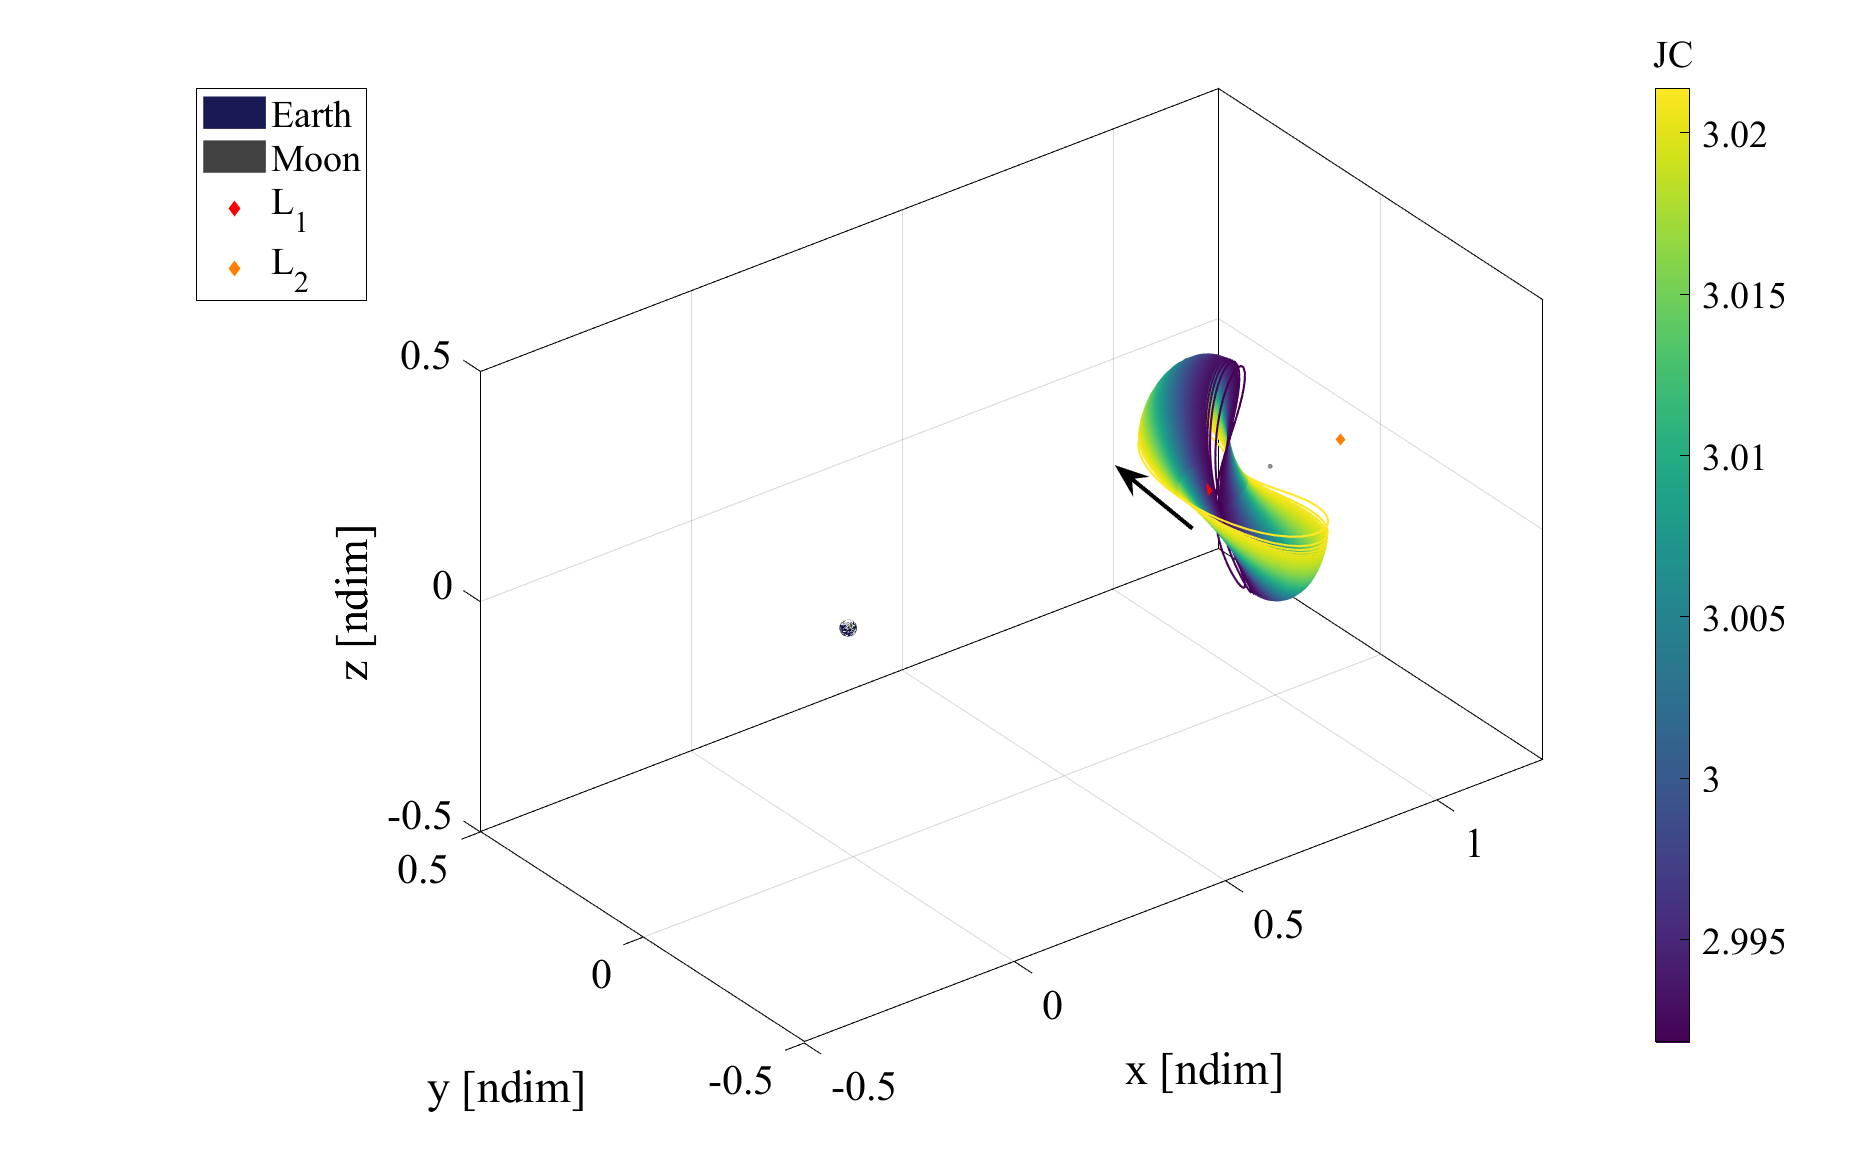
\includegraphics[width=0.9\textwidth]{figures/L1AxialFamily.pdf}
    \caption{Earth-Moon $L_{1}$ northeast axial orbit family.}
    \label{fig:L1Axial}
\end{figure}

\begin{figure}[ht]
    \centering
    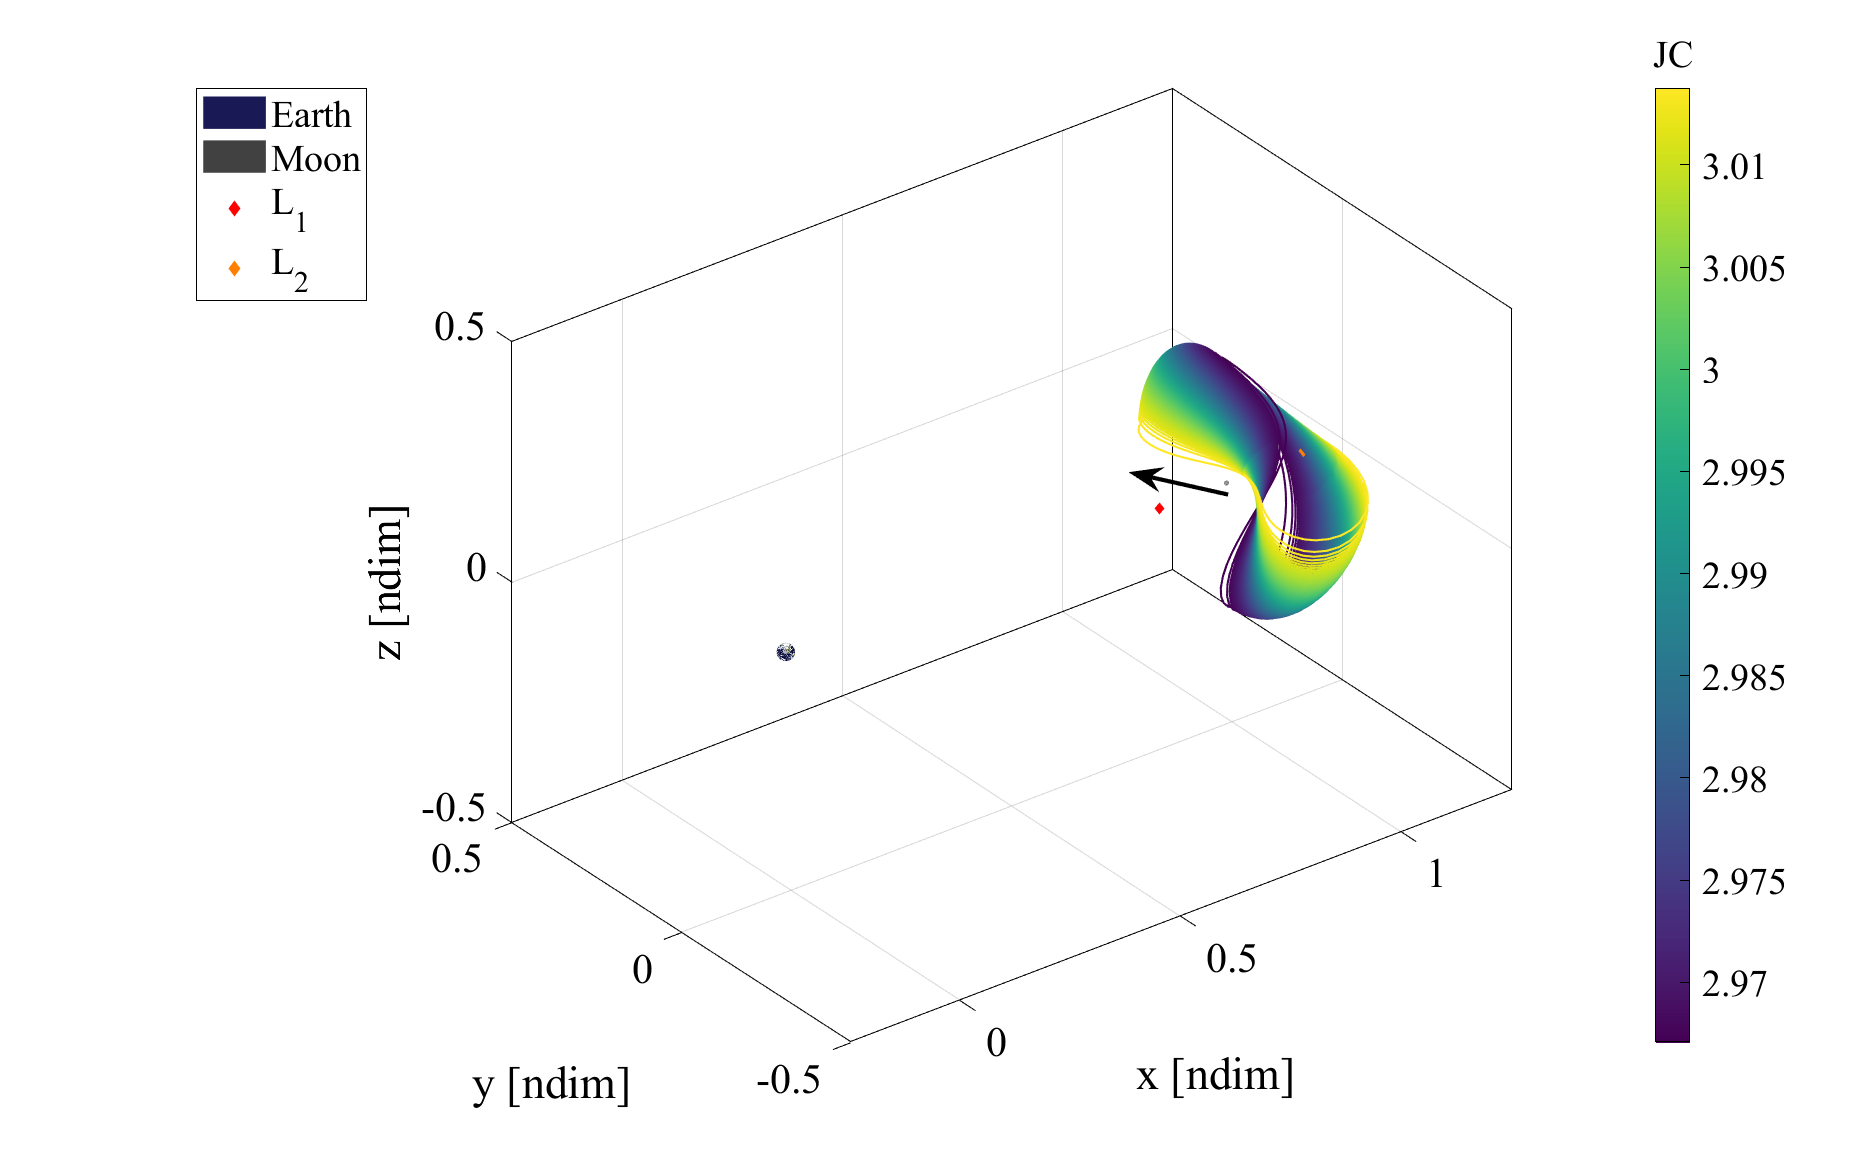
\includegraphics[width=0.9\textwidth]{figures/L2AxialFamily.pdf}
    \caption{Earth-Moon $L_{2}$ northwest axial orbit family.}
    \label{fig:L2Axial}
\end{figure}

\begin{figure}[ht]
    \begin{subfigure}[h]{0.4\linewidth}
        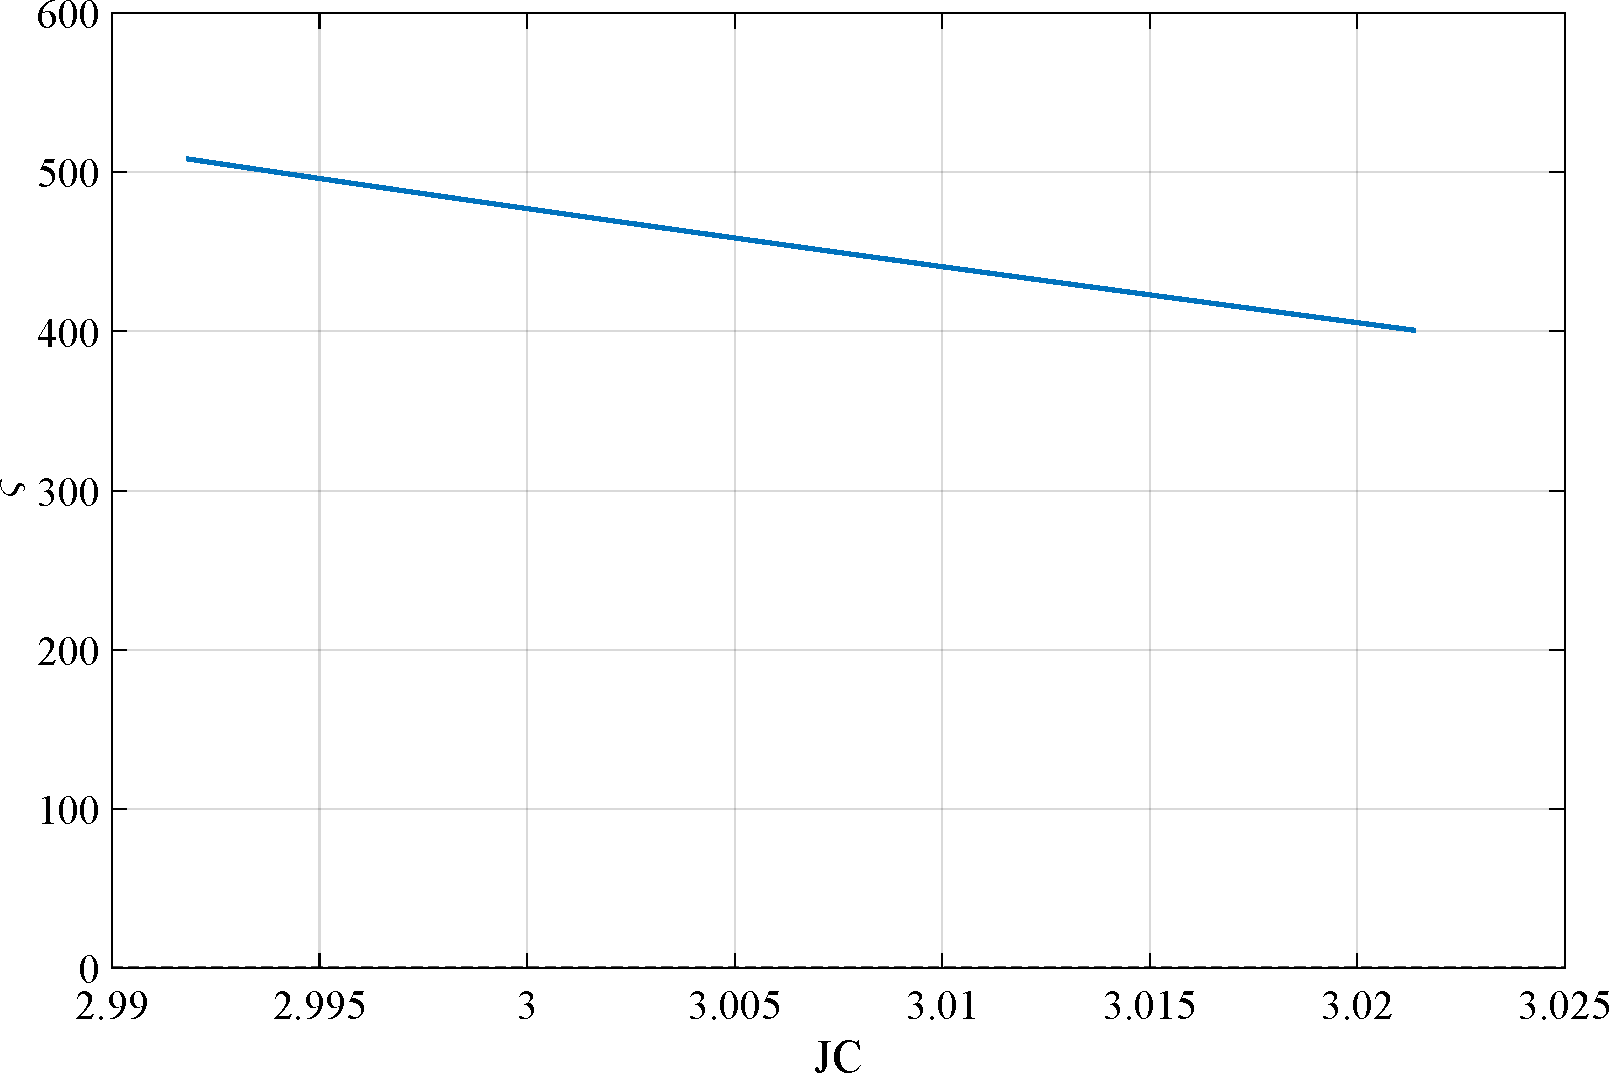
\includegraphics[width=\textwidth]{figures/L1AxialStability.pdf}
        \caption{$L_{1}$}
    \end{subfigure}
    \hfill
    \begin{subfigure}[h]{0.4\linewidth}
        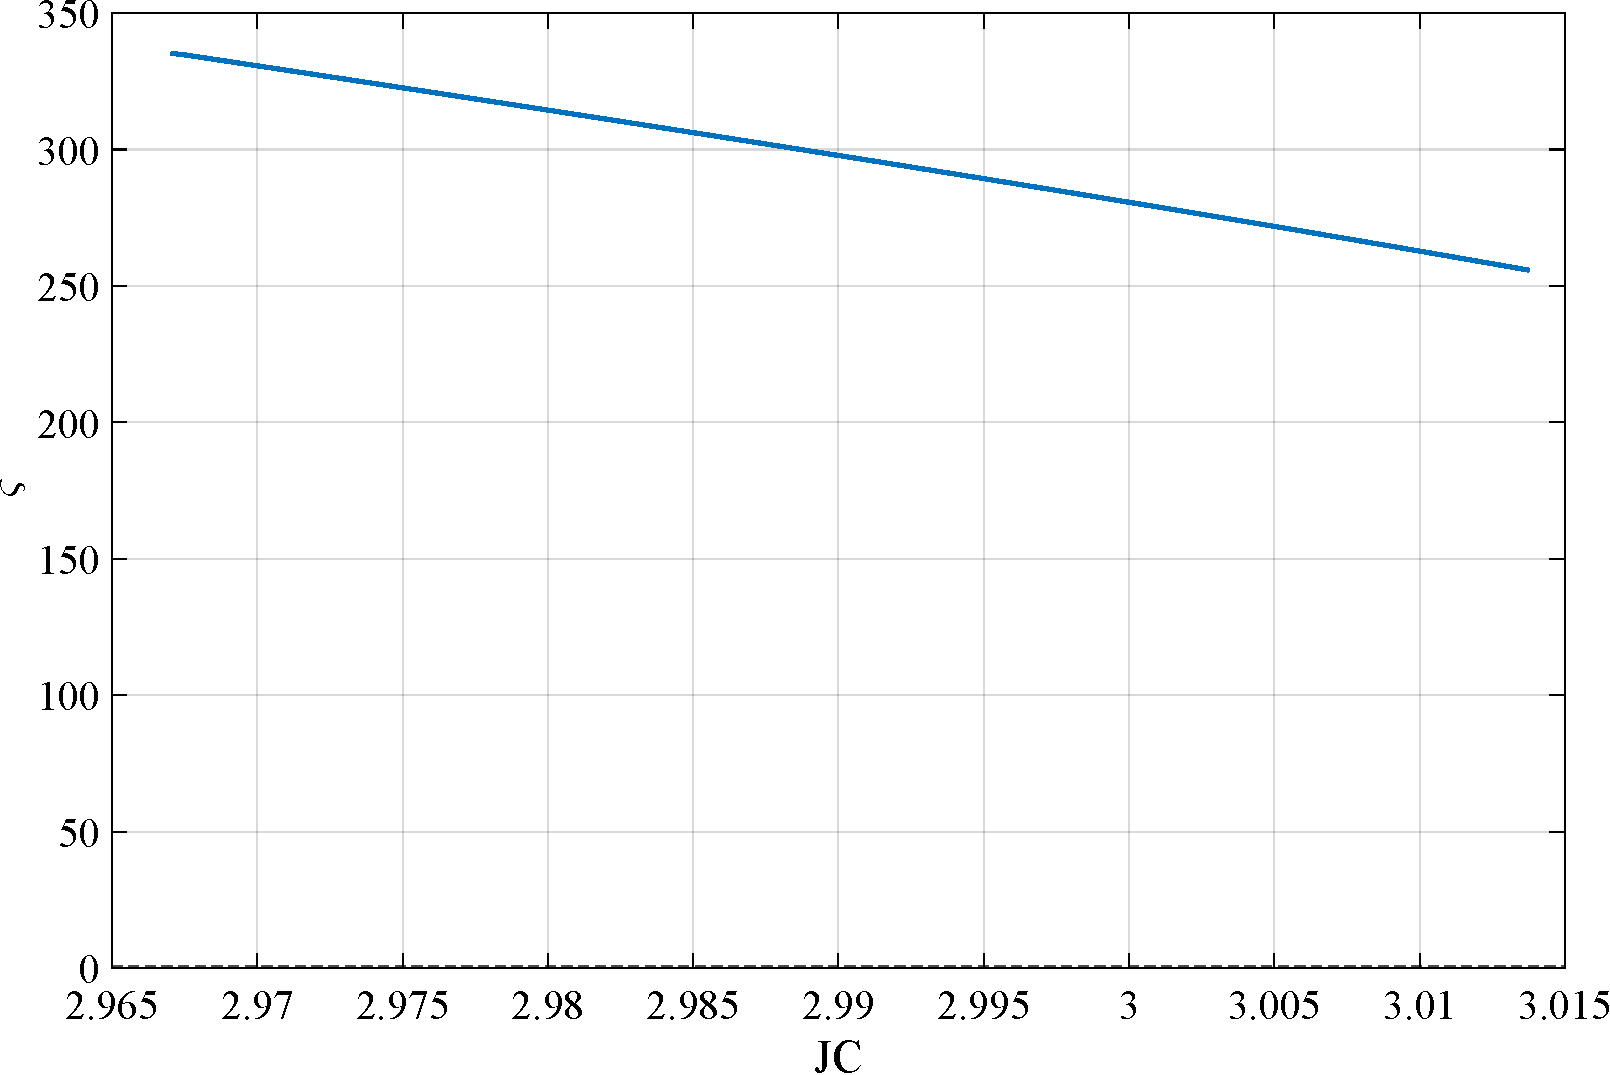
\includegraphics[width=\textwidth]{figures/L2AxialStability.pdf}
        \caption{$L_{2}$}
    \end{subfigure}
    \caption{Earth-Moon axial family stability index evolution.}
    \label{fig:axialStability}
\end{figure}

\subsection{Vertical Orbits}
\phantomsection
\subsubsection{A Vertical Targeter}
Vertical orbits benefit from double symmetry about both the $xz$- and $xy$-planes. This allows for
targeting only a quarter of the orbit, with a perpendicular crossing of the $xz$-plane on one end
of the arc and a perpendicular crossing of the $x$-axis on the other. Starting from the $xz$-plane
crossing:
\begin{equation}
    \Xbar=\begin{bmatrix}   x_{0}   &   z_{0}   &   \ydot_{0}   &   \tau    \end{bmatrix}^{T},
    \label{eq:verticalfreevar}
\end{equation}
\begin{equation}
    \Fbar(\Xbar)=\begin{bmatrix}    y_{f}   &   z_{f}   &   \xdot_{f}   &   C-C_{d} \end{bmatrix}^{T}=\zerobar,
    \label{eq:verticalconst}
\end{equation}
\begin{equation}
    DF(\Xbar)=\begin{bmatrix}   \phi_{21}                                                                   &   \phi_{23}                                               &   \phi_{25}   &   \ydot_{f}   \\
                                \phi_{31}                                                                   &   \phi_{33}                                               &   \phi_{35}   &   \zdot_{f}   \\
                                \phi_{41}                                                                   &   \phi_{43}                                               &   \phi_{45}   &   \xddot_{f}  \\
                                2x_{0}-\frac{2(x_{0}+\mu)(1-\mu)}{d^{3}}-\frac{2\mu(x_{0}-1+\mu)}{r^{3}}    &   -\frac{2z_{0}(1-\mu)}{d^{3}}-\frac{2z_{0}\mu}{r^{3}}    &   -2\ydot_{0} &   0           \end{bmatrix}.
    \label{eq:verticaljacobian}
\end{equation}
The result of this targeting will provide the initial state ($y_{0}=\xdot_{0}=\zdot_{0}=0$) at the
perpendicular crossing of the $xz$-plane (top/bottom of the orbit) and one-quarter of the
propagation time for a periodic vertical orbit.

\subsubsection{Converged Vertical Families}
The vertical orbit family bifurcates from the end of the axial family when the axial orbit
intersects itself and resembles a figure-eight. Stepping in one direction shrinks the orbits as the
family collapses down to its origin Lagrange point. The other direction expands the orbits until
they look like clam shells, demonstrated for the $L_{1}$ family in \cref{fig:L1Vertical}. Similar
behavior occurs with the $L_{2}$ vertical family in \cref{fig:L2Vertical}.
\cref{fig:verticalStability} shows the stability indices for these two families; $L_{3}$ verticals
are not used in this investigation.

\begin{figure}[ht]
    \centering
    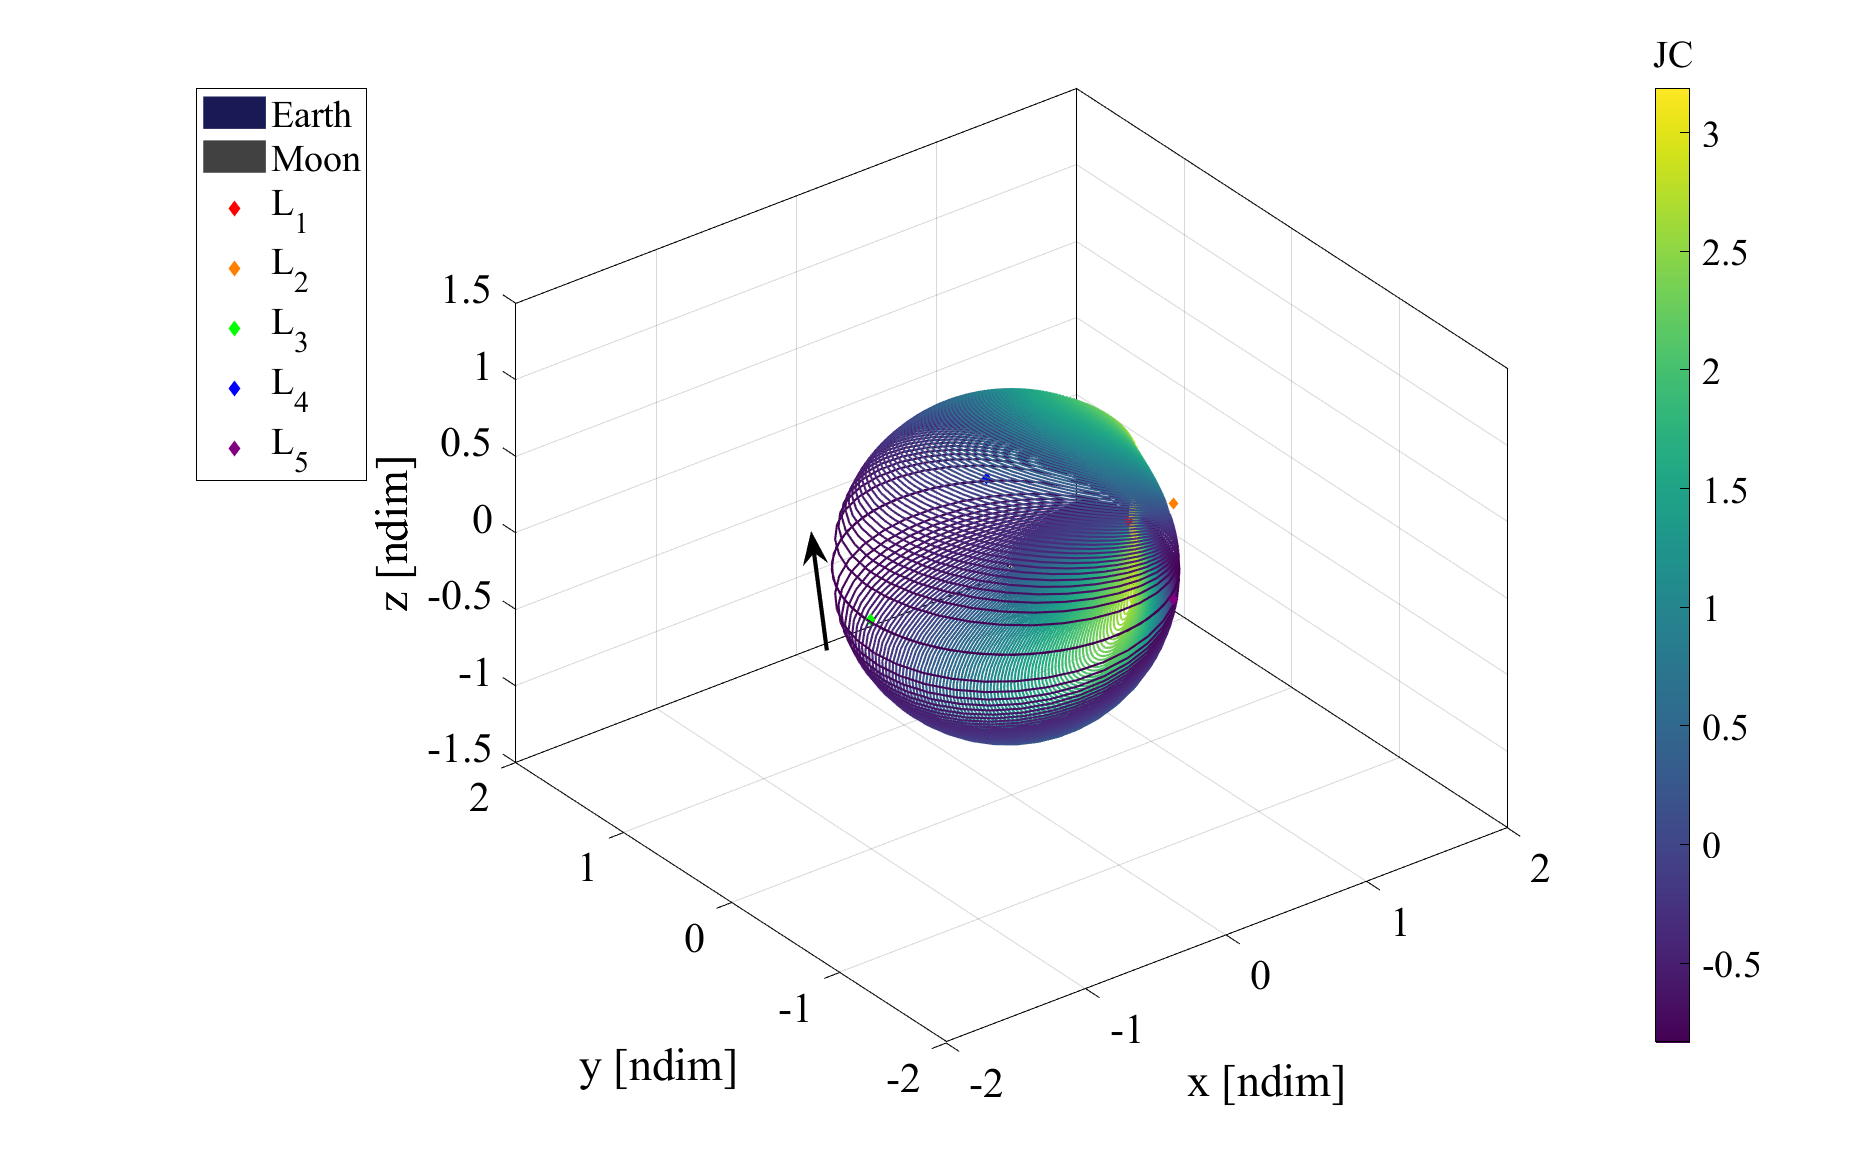
\includegraphics[width=0.9\textwidth]{figures/L1VerticalFamily.pdf}
    \caption{Earth-Moon $L_{1}$ vertical orbit family.}
    \label{fig:L1Vertical}
\end{figure}

\begin{figure}[ht]
    \centering
    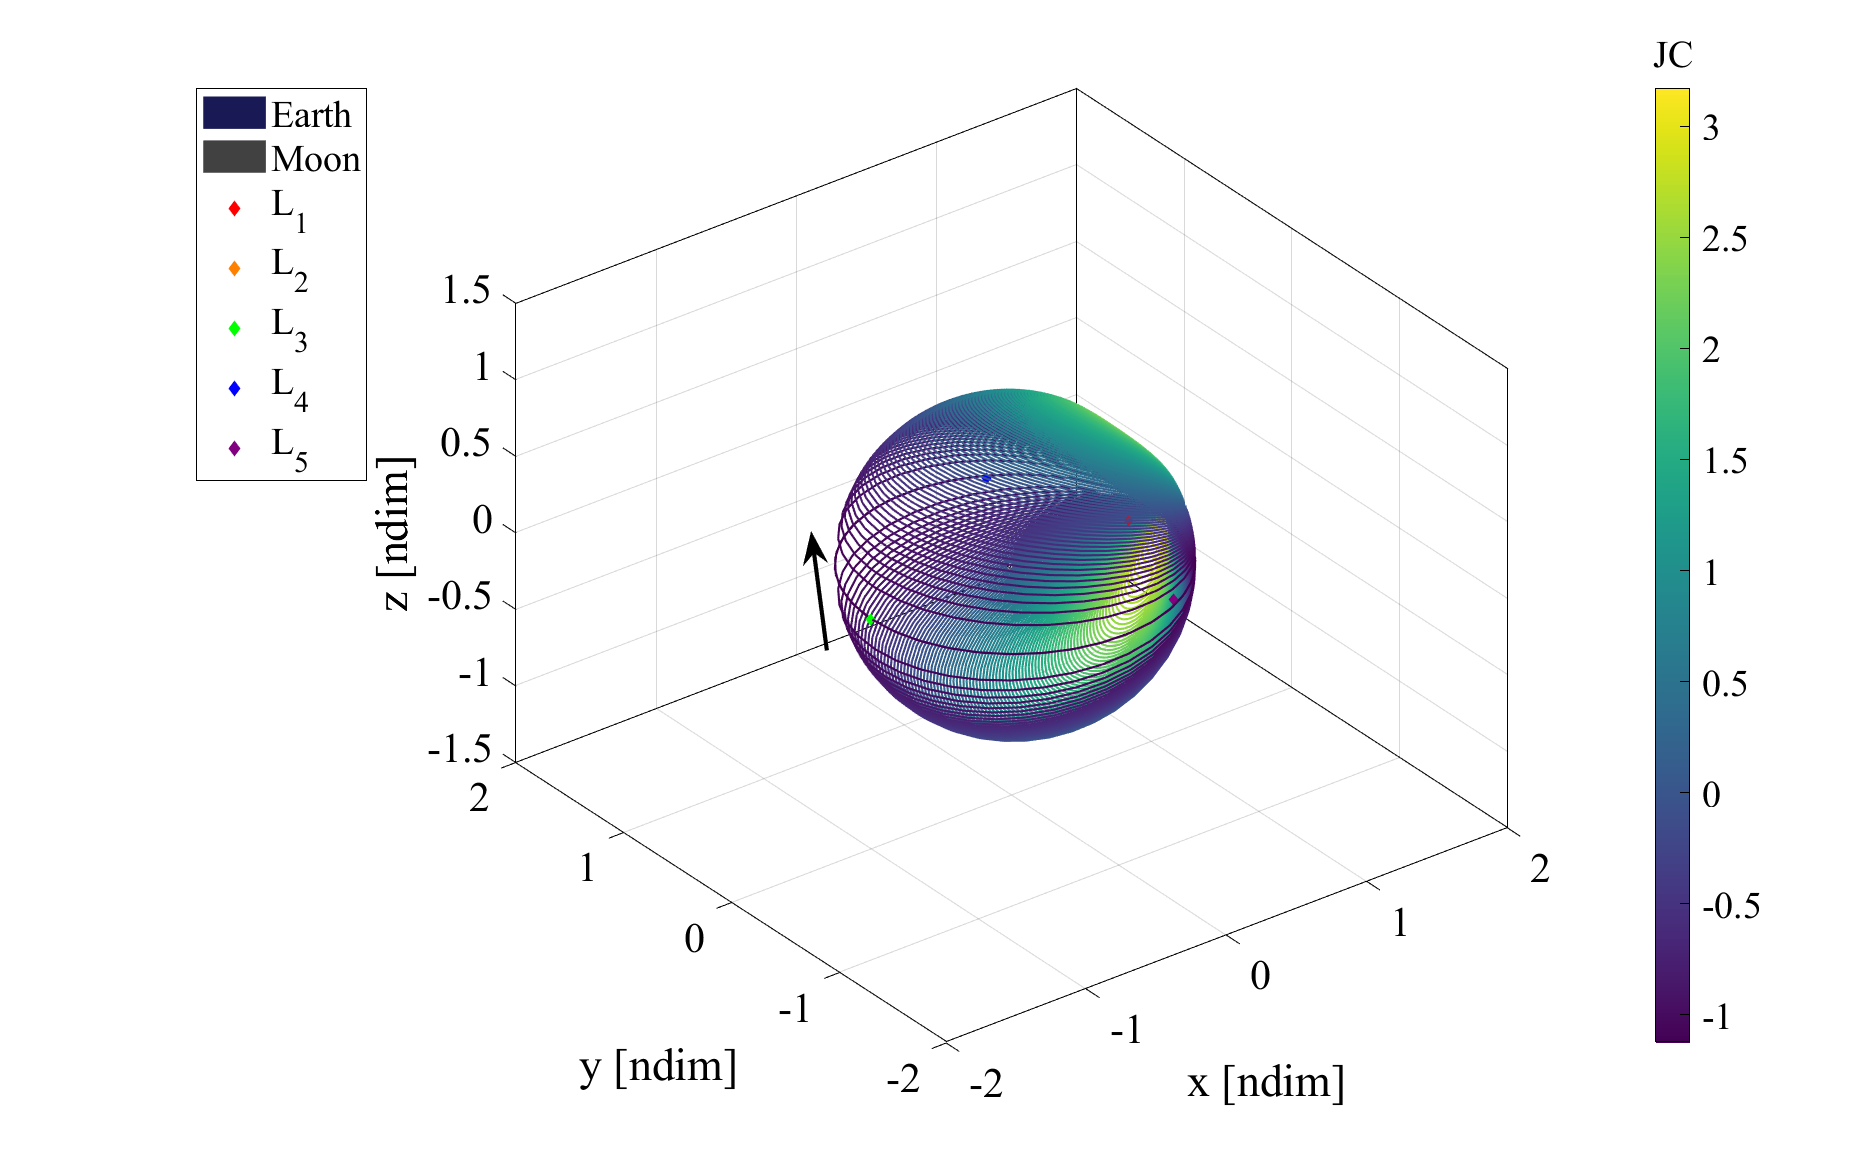
\includegraphics[width=0.9\textwidth]{figures/L2VerticalFamily.pdf}
    \caption{Earth-Moon $L_{2}$ vertical orbit family.}
    \label{fig:L2Vertical}
\end{figure}

\begin{figure}[ht]
    \begin{subfigure}[h]{0.4\linewidth}
        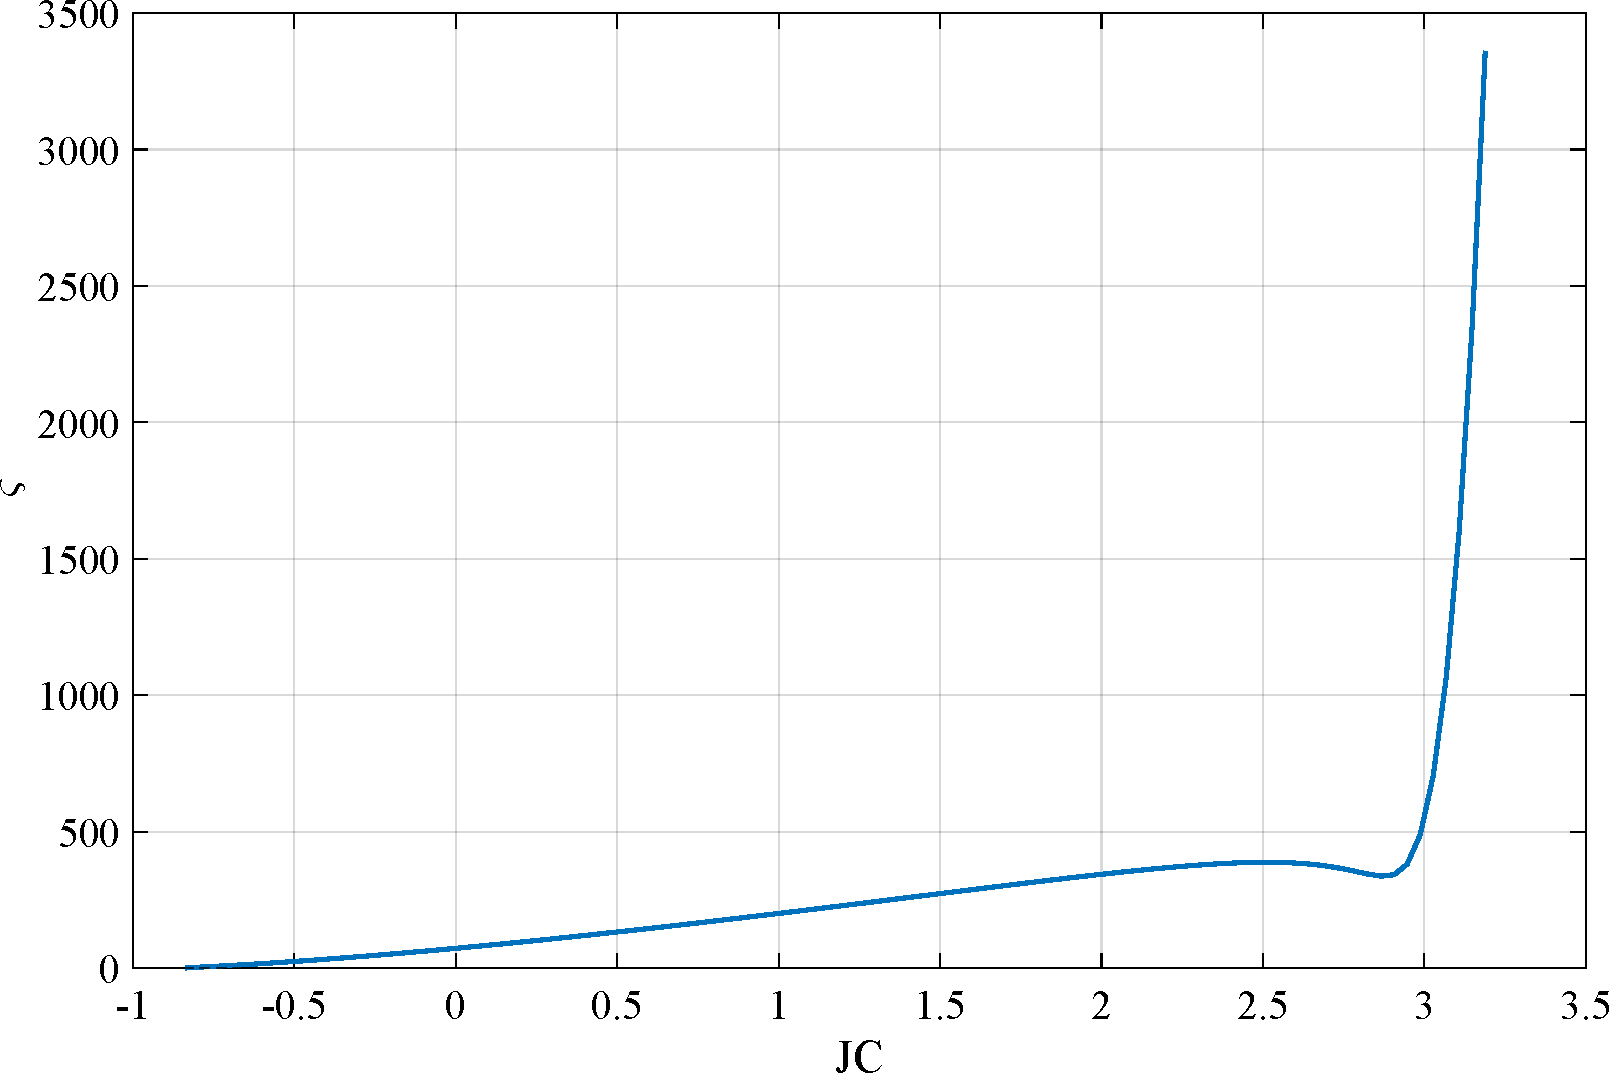
\includegraphics[width=\textwidth]{figures/L1VerticalStability.pdf}
        \caption{$L_{1}$}
    \end{subfigure}
    \hfill
    \begin{subfigure}[h]{0.4\linewidth}
        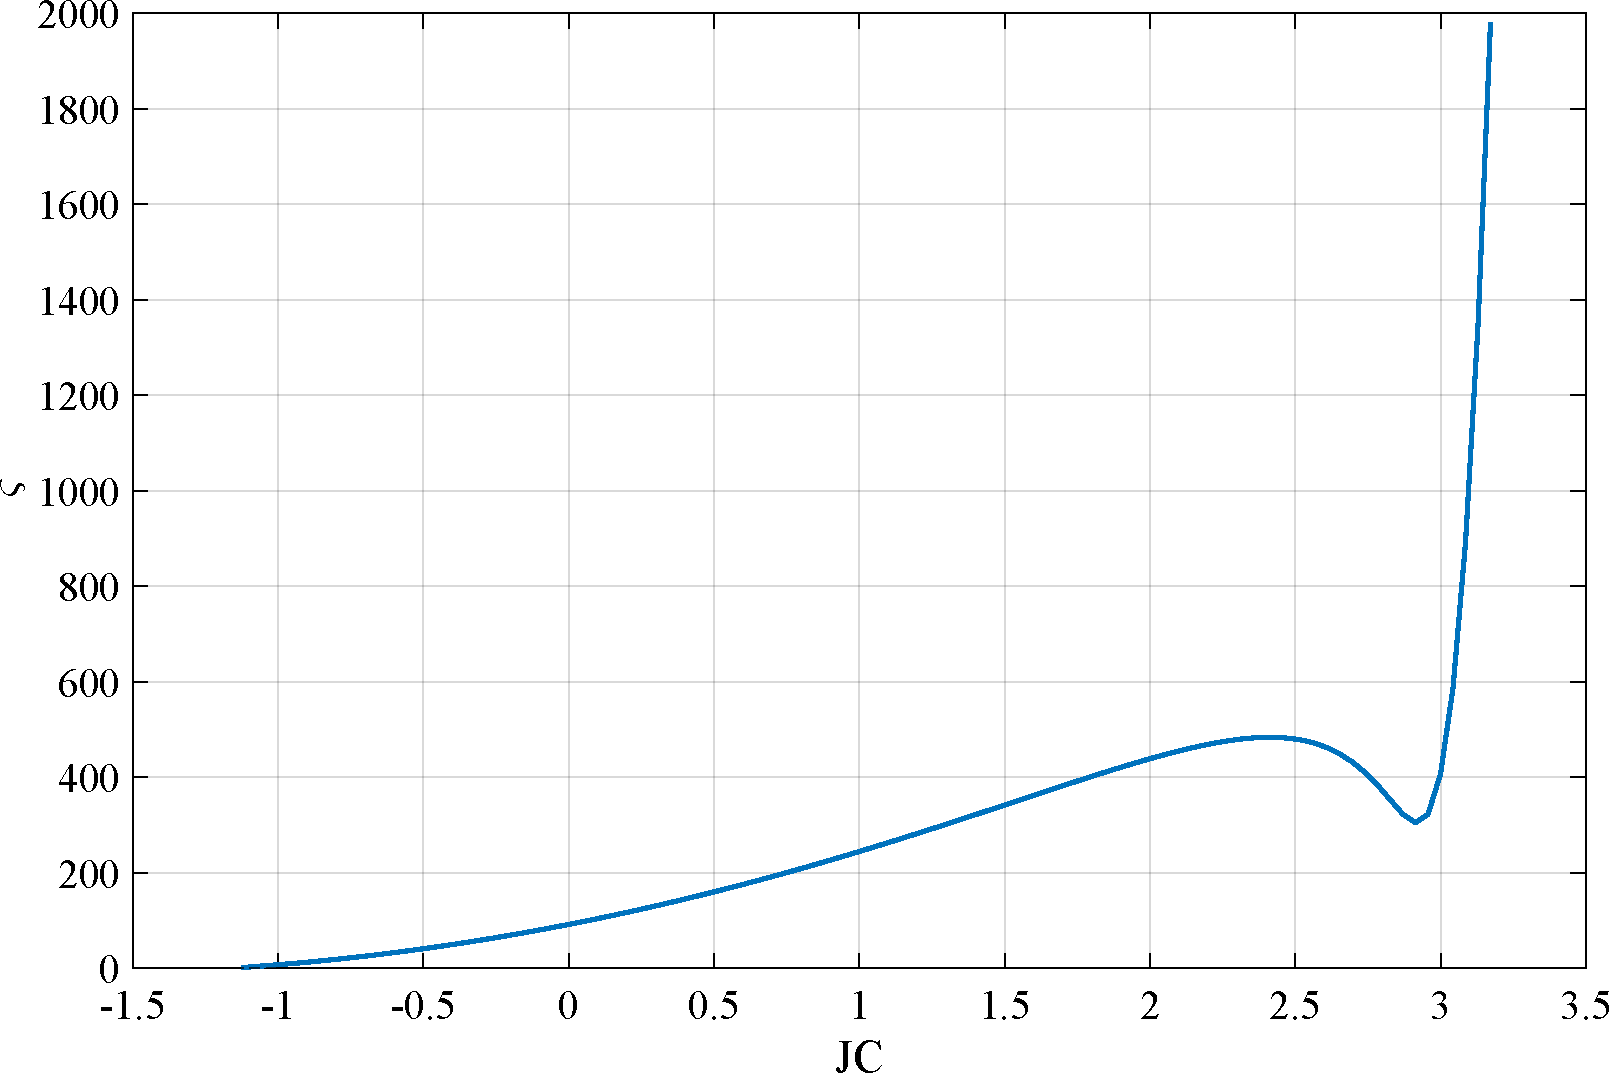
\includegraphics[width=\textwidth]{figures/L2VerticalStability.pdf}
        \caption{$L_{2}$}
    \end{subfigure}
    \caption{Earth-Moon vertical family stability index evolution.}
    \label{fig:verticalStability}
\end{figure}

\subsection{Equilateral Long Period Orbits}
\phantomsection
\subsubsection{A Planar Equilateral Orbit Targeter}
Similar to the Lyapunov orbits around the colinear equilibrium points, there are planar orbits
around the equilateral equilibrium points $L_{4}$ and $L_{5}$; however, they do not have symmetry
that can be exploited. Therefore, the full period of the orbit needs to be targeted, constraining
periodicity between the propagation start and end points. Note that since the Jacobi constant of a
propagated trajectory is naturally constrained, constraining periodicity only requires constraining
five out of the six states (three out of the four for a planar problem):
\begin{equation}
    \Xbar=\begin{bmatrix}   x_{0}   &   \xdot_{0}   &   \ydot_{0}   &   \tau    \end{bmatrix}^{T},
    \label{eq:longfreevar}
\end{equation}
\begin{equation}
    \Fbar(\Xbar)=\begin{bmatrix}    x_{f}-x_{0} &   y_{f}-y_{0} &   \xdot_{f}-\xdot_{0} &   C-C_{d} \end{bmatrix}^{T}=\zerobar,
    \label{eq:longconst}
\end{equation}
\begin{equation}
    DF(\Xbar)=\begin{bmatrix}   \phi_{11}-1                                                                 &   \phi_{14}   &   \phi_{15}   &   \xdot_{f}   \\
                                \phi_{21}                                                                   &   \phi_{24}   &   \phi_{25}   &   \ydot_{f}   \\
                                \phi_{41}                                                                   &   \phi_{44}-1 &   \phi_{45}   &   \xddot_{f}  \\
                                2x_{0}-\frac{2(x_{0}+\mu)(1-\mu)}{d^{3}}-\frac{2\mu(x_{0}-1+\mu)}{r^{3}}    &   -2\xdot_{0} &   -2\ydot_{0} &   0           \end{bmatrix}.
    \label{eq:longjacobian}
\end{equation}
Since $z=\zdot=0$, this targeter provides five of the six initial state variables and the full
period for the planar equilateral orbit.

\subsubsection{Equilateral Long Period Orbit Initial Guess}
Initial guesses for the planar equilateral orbits close to the Lagrange point can come from linear
variational equations of motion about the equilibrium point:
\begin{equation}
    x_{0}=x_{L}+\xi,
    \label{eq:xvareq}
\end{equation}
\begin{equation}
    y_{0}=y_{L}+\eta,
    \label{eq:yvareq}
\end{equation}
\begin{equation}
    \xdot_{0}=\alpha s,
    \label{eq:xdotvareq}
\end{equation}
\begin{equation}
    \ydot_{0}=\beta s,
    \label{eq:ydotvareq}
\end{equation}
where $\xi$ and $\eta$ are chosen variations from the Lagrange point,
\begin{equation}
    s=\Im(\lambda),
    \label{eq:seq}
\end{equation}
\begin{equation}
    \alpha=\frac{\xi\frac{\partial U}{\partial x\partial y}+\eta(\frac{\partial u}{\partial y\partial y}+s^{2})}{2s},
    \label{eq:alphaeq}
\end{equation}
\begin{equation}
    \beta=-\frac{\xi(\frac{\partial U}{\partial x\partial x}+s^{2})+\eta\frac{\partial U}{\partial x\partial y}}{2s}.
    \label{eq:betaeq}
\end{equation}
The linearization has two frequencies, short and long, and the choice of frequency determines
$\lambda$. The short period orbits are not used in this investigation, so for long period orbits:
\begin{equation}
    \lambda=\sqrt{\frac{\sqrt{1-27\mu(1-\mu)}-1}{2}}.
    \label{eq:lambdaeq}
\end{equation}

For consistency, $y_{0}$ is chosen to be the $y$-value of the Lagrange point $y_{L}$ with $\eta=0$.
The initial guess for the period is also determined by the choice of frequency:
\begin{equation}
    \tau=2\pi s.
    \label{eq:taueq}
\end{equation}

\subsubsection{Converged Equilateral Long Period Orbit Families}
Since the CR3BP is symmetric about the $xz$-plane, all $L_{4}$ orbit families can be mirrored
across that plane to find the $L_{5}$ families and vice versa. This is done by flipping the signs
of $y$, $\xdot$, and $\zdot$. Therefore, \cref{fig:longPeriod} shows portions of both equilateral
long period orbit families in the Earth-Moon system and \cref{fig:longPeriodStability} shows their
stability indices. 

\begin{figure}[ht]
    \centering
    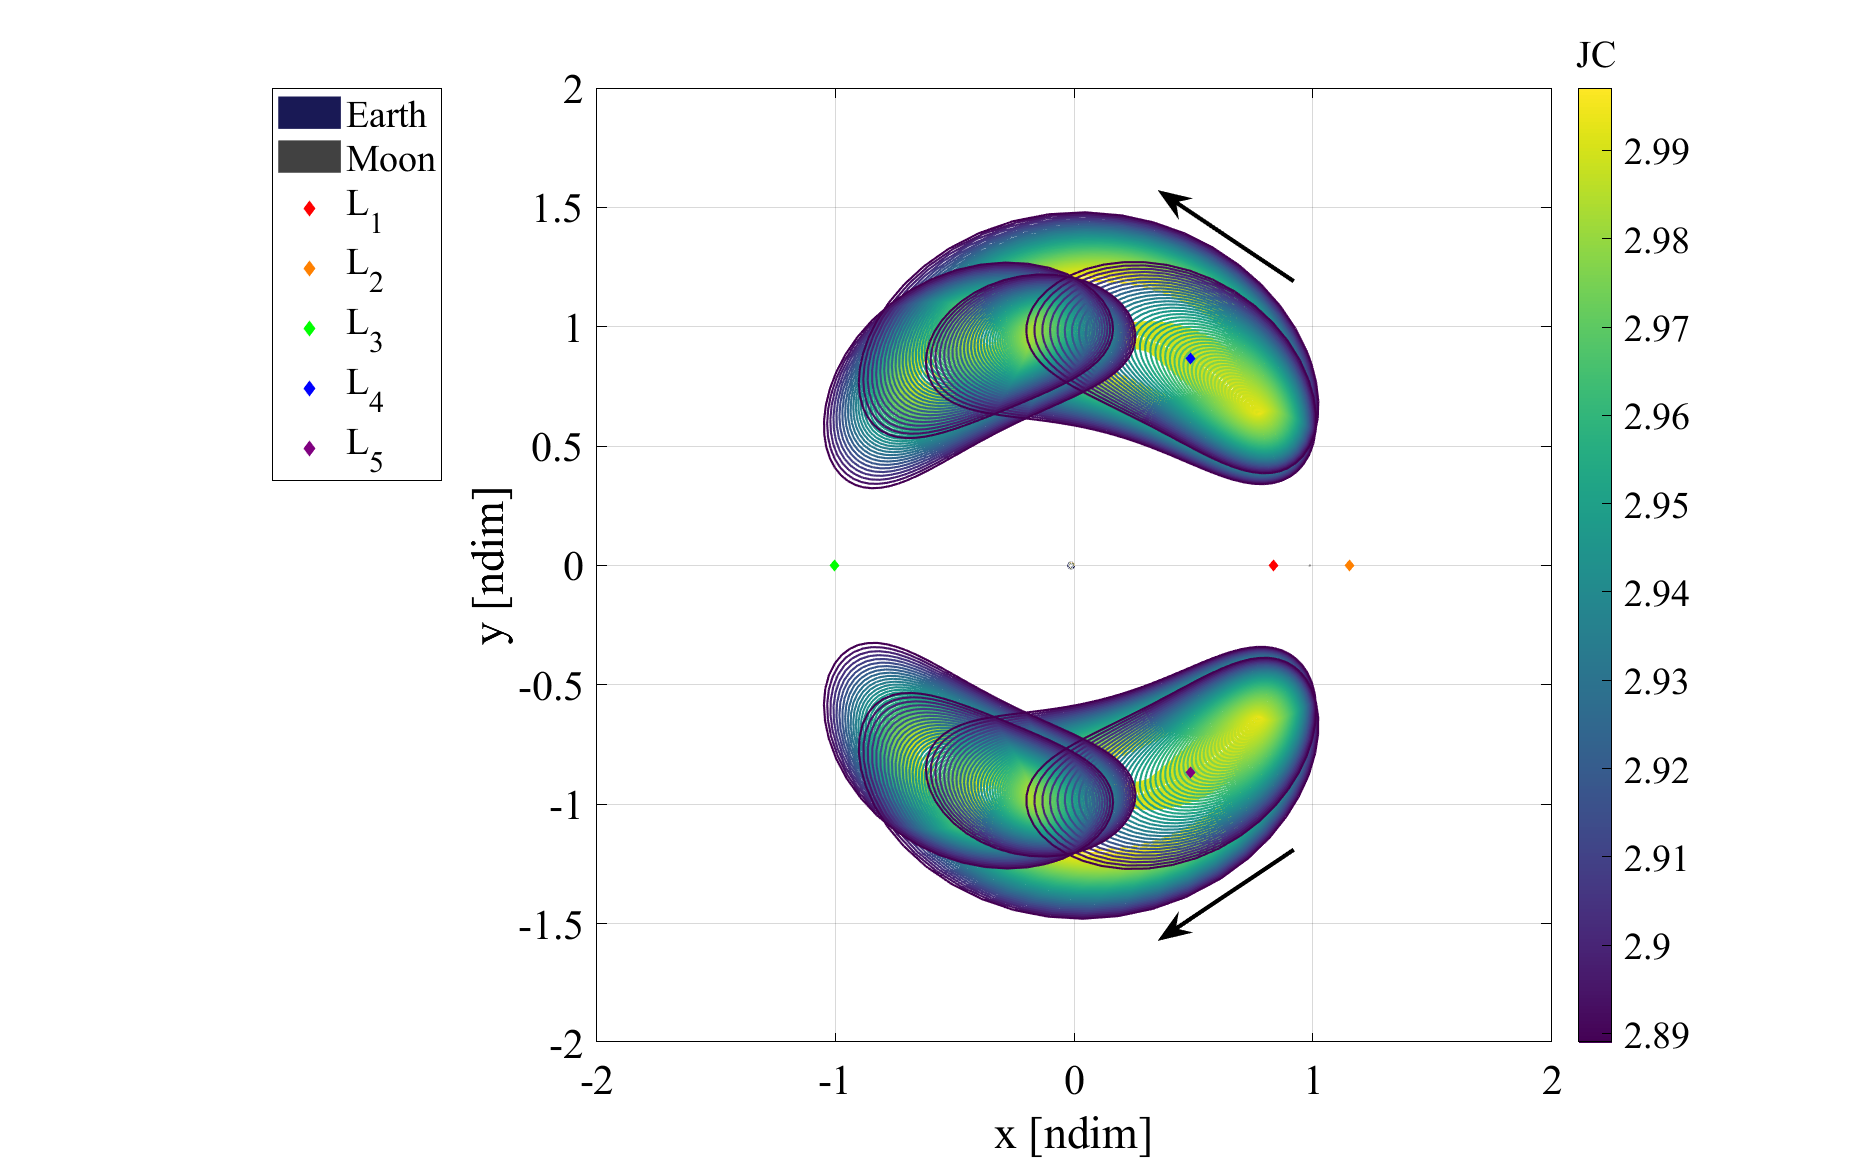
\includegraphics[width=0.9\textwidth]{figures/LongPeriodFamily.pdf}
    \caption{Earth-Moon $L_{4}$ and $L_{5}$ equilateral long period orbit families.}
    \label{fig:longPeriod}
\end{figure}

\begin{figure}[ht]
    \centering
    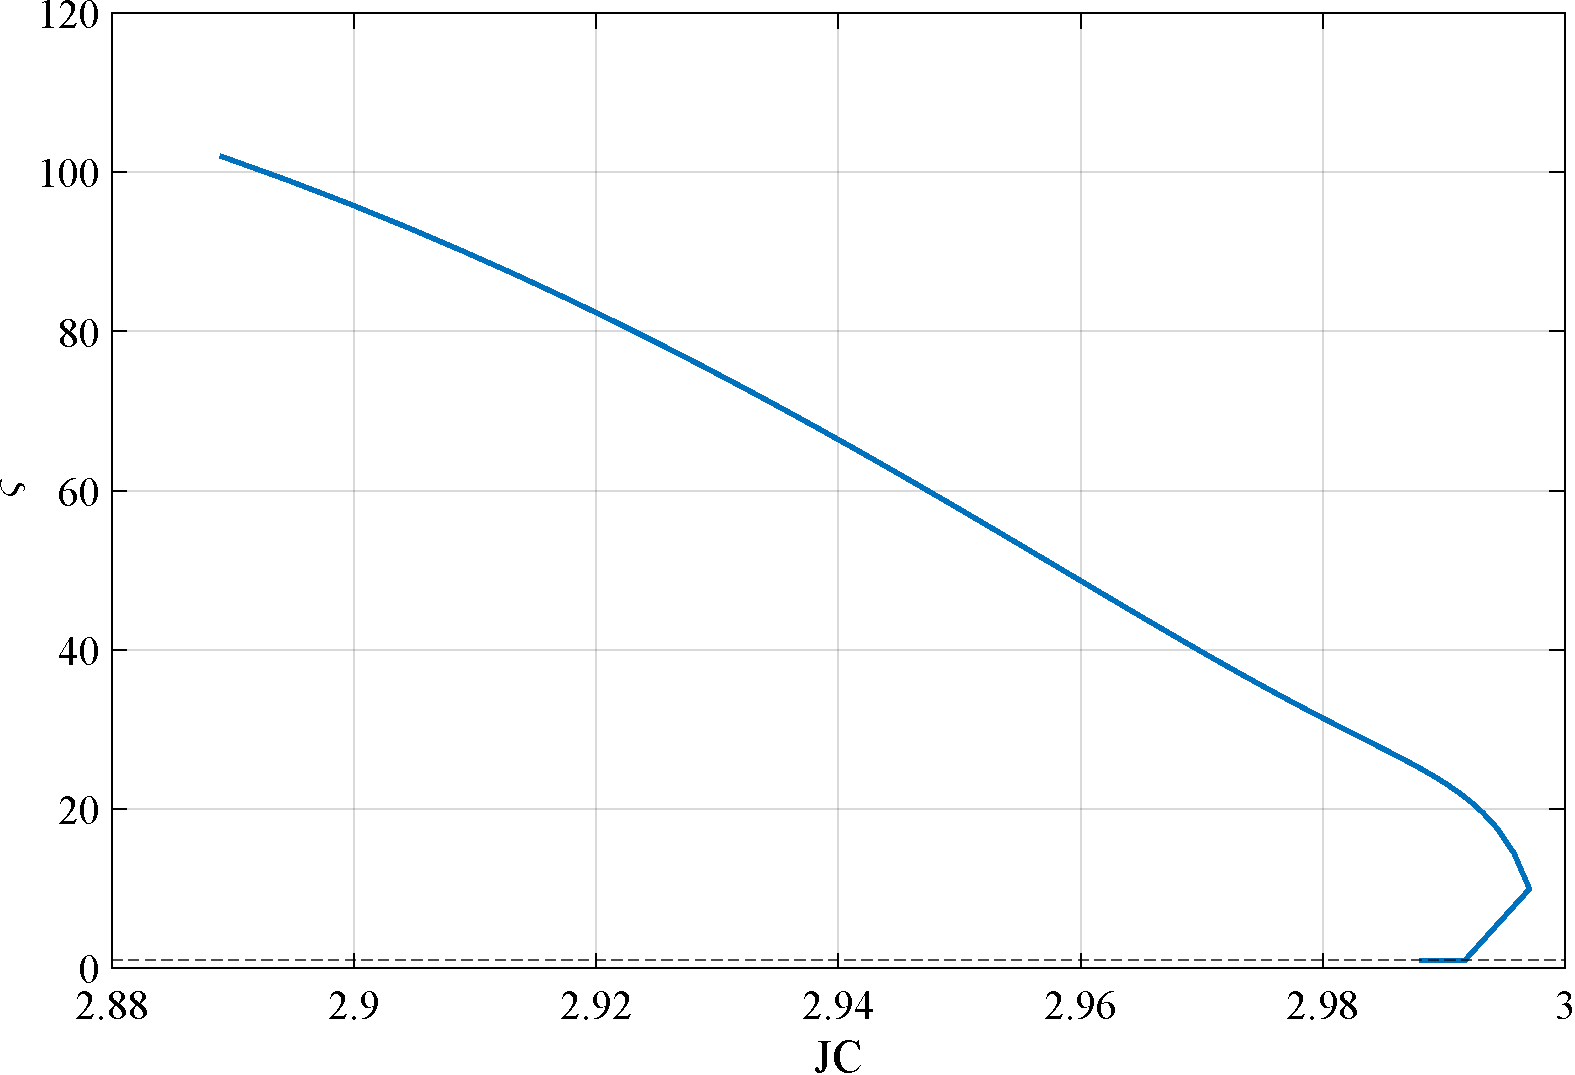
\includegraphics[width=0.5\textwidth]{figures/LongPeriodStability.pdf}
    \caption{Earth-Moon equilateral long period orbit family stability index evolution.}
    \label{fig:longPeriodStability}
\end{figure}

\subsection{Equilateral Axial Orbits}
\phantomsection
\subsubsection{A Spatial Equilateral Orbit Targeter}
While axial orbits exist around $L_{4}$ and $L_{5}$, unlike their colinear counterparts, these
axial families bifurcate from the $L_{1}$ halo family. Like the planar equilateral orbits, symmetry
cannot be exploited to aid the targeting process, so periodicity must be targeted instead:
\begin{equation}
    \Xbar=\begin{bmatrix}   x_{0}   &   y_{0}   &   \xdot_{0}   &   \ydot_{0}   &   \zdot_{0}   \tau    \end{bmatrix}^{T},
    \label{eq:eqaxialfreevar}
\end{equation}
\begin{equation}
    \Fbar(\Xbar)=\begin{bmatrix}    x_{f}-x_{0} &   y_{f}-y_{0} &   \xdot_{f}-\xdot_{0} &   \ydot_{f}-\ydot_{0} &   \zdot_{f}-\zdot_{0} &   C-C_{d} \end{bmatrix}^{T}=\zerobar,
    \label{eq:eqaxialconst}
\end{equation}
\begin{multline}
    DF(\Xbar)=\\
    \begin{bmatrix} \phi_{11}-1                                                                 &   \phi_{12}                                                   &   \phi_{14}   &   \phi_{15}   &   \phi_{16}   &   \xdot_{f}   \\
                    \phi_{21}                                                                   &   \phi_{22}-1                                                 &   \phi_{24}   &   \phi_{25}   &   \phi_{26}   &   \ydot_{f}   \\
                    \phi_{41}                                                                   &   \phi_{42}                                                   &   \phi_{44}-1 &   \phi_{45}   &   \phi_{46}   &   \xddot_{f}  \\
                    \phi_{51}                                                                   &   \phi_{52}                                                   &   \phi_{54}   &   \phi_{55}-1 &   \phi_{56}   &   \yddot_{f}  \\
                    \phi_{61}                                                                   &   \phi_{62}                                                   &   \phi_{64}   &   \phi_{65}   &   \phi_{66}-1 &   \zddot_{f}  \\
                    2x_{0}-\frac{2(x_{0}+\mu)(1-\mu)}{d^{3}}-\frac{2\mu(x_{0}-1+\mu)}{r^{3}}    &   2y_{0}-\frac{2y_{0}(1-\mu)}{d^{3}}-\frac{2y_{0}\mu}{r^{3}}  &   -2\xdot_{0} &   -2\ydot_{0} &   -2\zdot_{0} &   0           \end{bmatrix}.
    \label{eq:eqaxialjacobian}
\end{multline}

\subsubsection{Converged Equilateral Axial Families}
The pseudo-arclength method can be used to obtain the initial guess for the equilateral axial
family. Stepping in one direction will produce the $L_{4}$ family while stepping in the other
produces the $L_{5}$ family. These are both shown in \cref{fig:eqAxial}.
\cref{fig:eqAxialStability} shows the stability indices for these families. As hinted at by the end
of these axial families, $L_{4}$ and $L_{5}$ vertical families also exist in the Earth-Moon system
but are not used in this investigation.

\begin{figure}[ht]
    \centering
    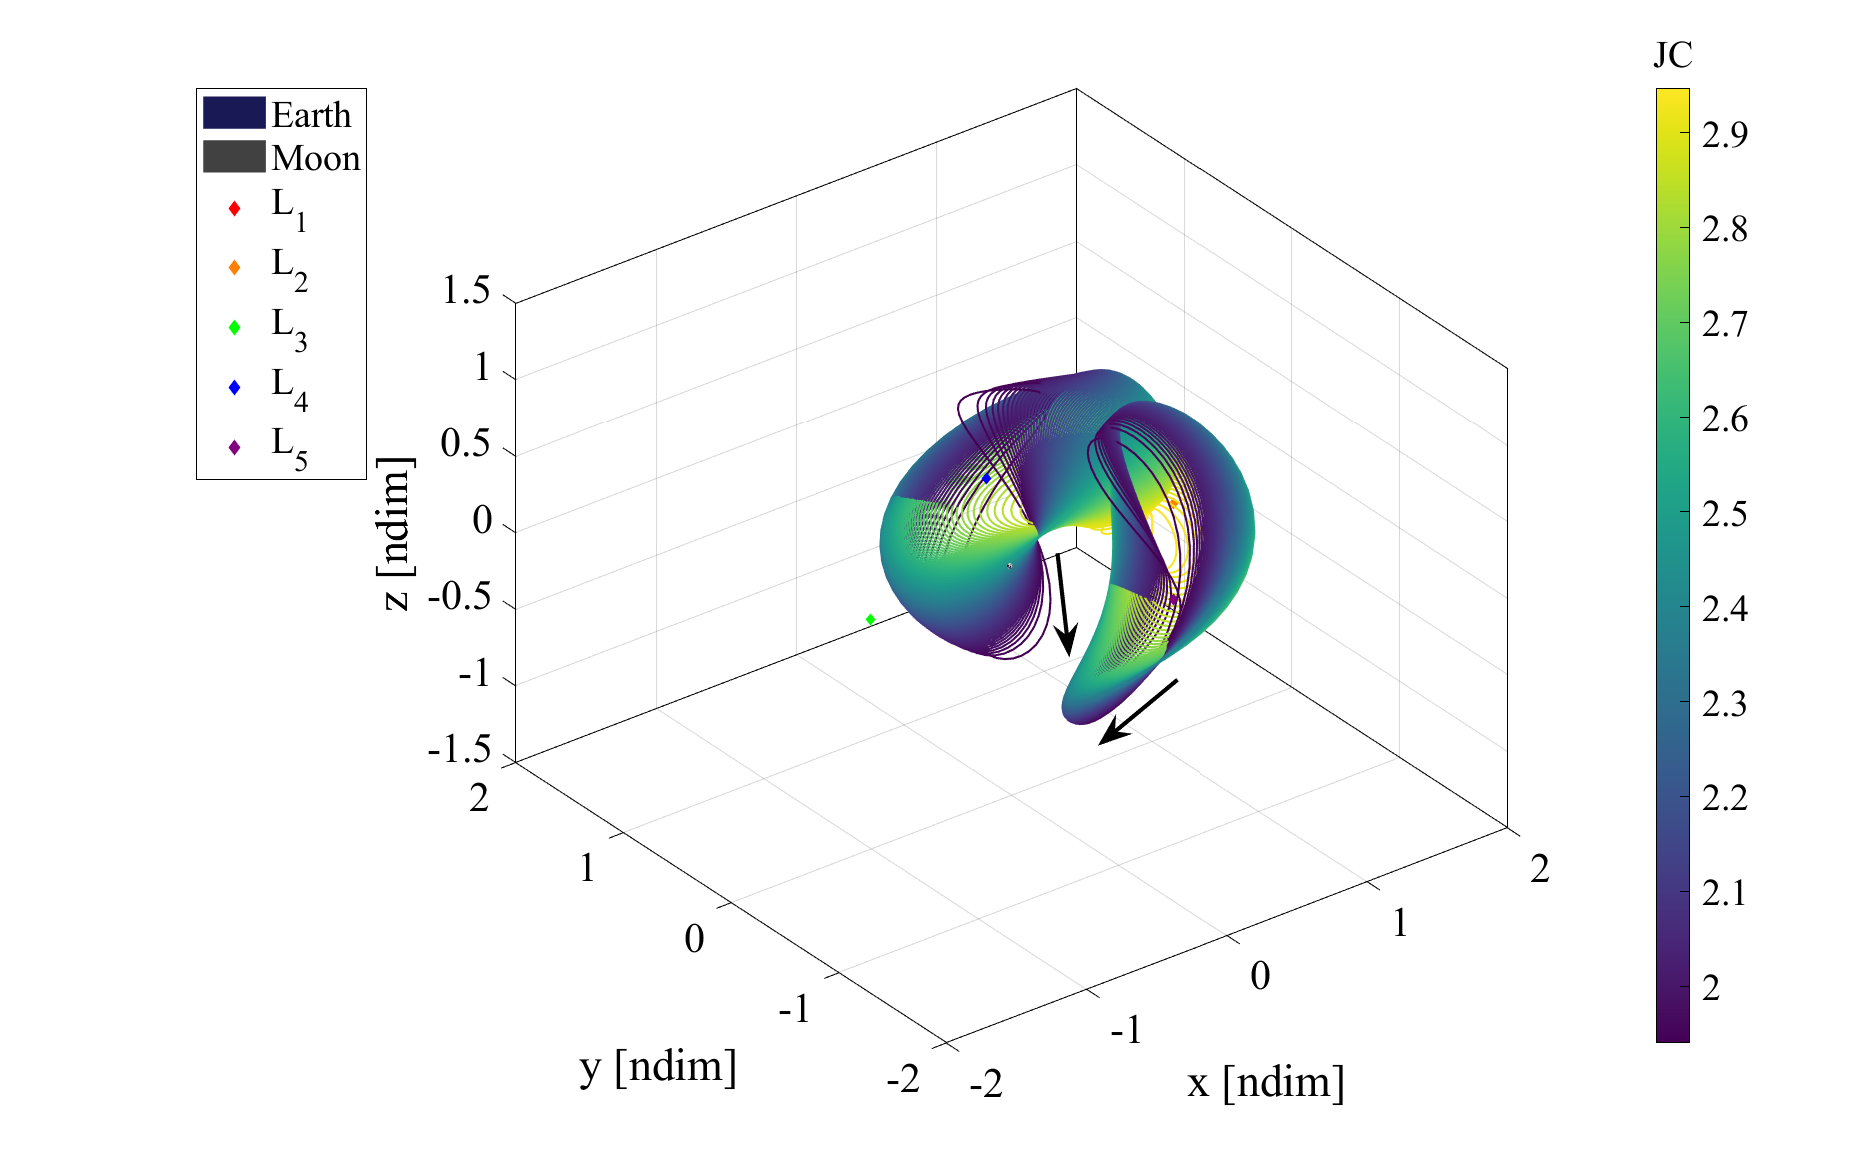
\includegraphics[width=0.9\textwidth]{figures/EquilateralAxialFamily.pdf}
    \caption{Earth-Moon $L_{4}$ and $L_{5}$ equilateral axial families.}
    \label{fig:eqAxial}
\end{figure}

\begin{figure}[ht]
    \centering
    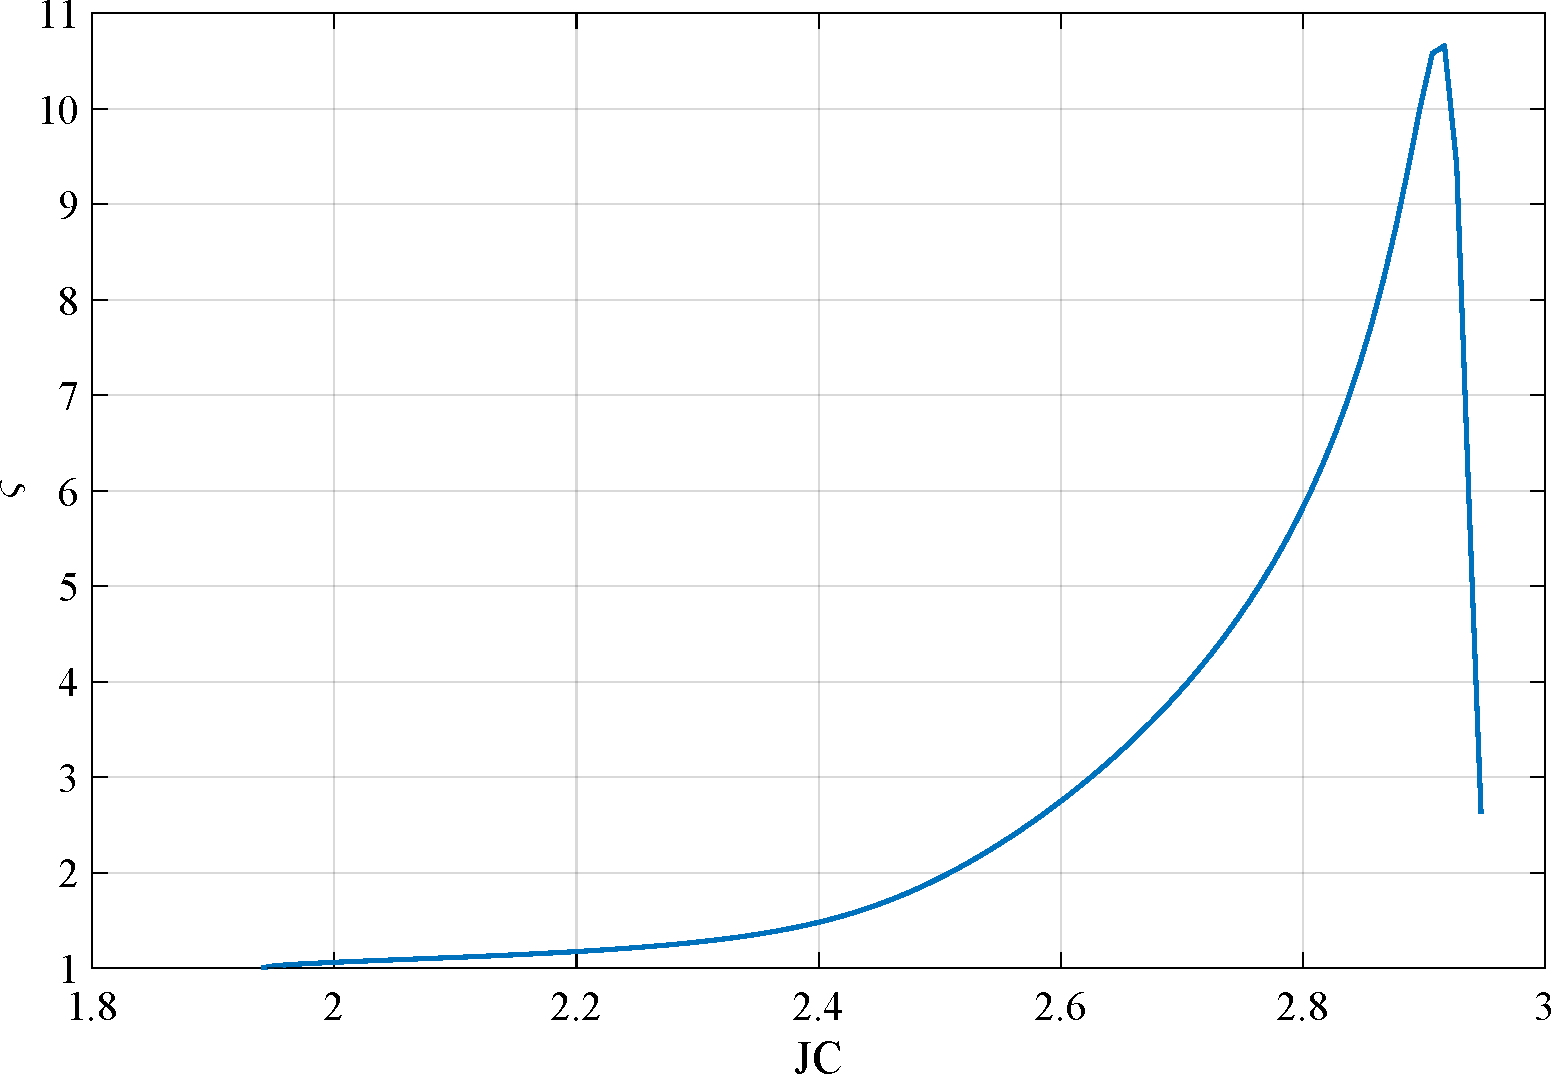
\includegraphics[width=0.5\textwidth]{figures/EquilateralAxialStability.pdf}
    \caption{Earth-Moon equilateral axial family stability index evolution.}
    \label{fig:eqAxialStability}
\end{figure}

\subsection{Resonant Orbits}
Many other types of CR3BP orbits are not associated with a Lagrange point. Some of these orbit
families are known as resonant orbits because their periods are resonant or close to resonant with
the Moon's' period. These orbits are still periodic in the rotating frame but are also periodic or
close to periodic in an inertial frame. Individual orbits also tend to span more of the Earth-Moon
system than the Lagrange point orbits. For more details on how to determine initial guesses and
correct these orbits, Gupta\cite{Gupta:2020} and Sadaka\cite{Sadaka:2023} provide extensive
overviews and initial conditions. A couple of unstable resonant orbit families are used in this
investigation and so they are shown here.

\phantomsection
\subsubsection{Converged 2:1a Resonant Orbit Family}
The unstable section of the 2:1 resonant orbit family (denoted the 2:1a resonant orbit family by
Sadaka) is shown in \cref{fig:2_1aResonant}\cite{Sadaka:2023}. These orbits travel around the
Earth roughly twice for every time the Moon revolves around it, which becomes more evident when
the trajectories are viewed in an inertial frame. \cref{fig:2_1aResonantStability} shows the
stability index evolution for this family.

\begin{figure}[ht]
    \centering
    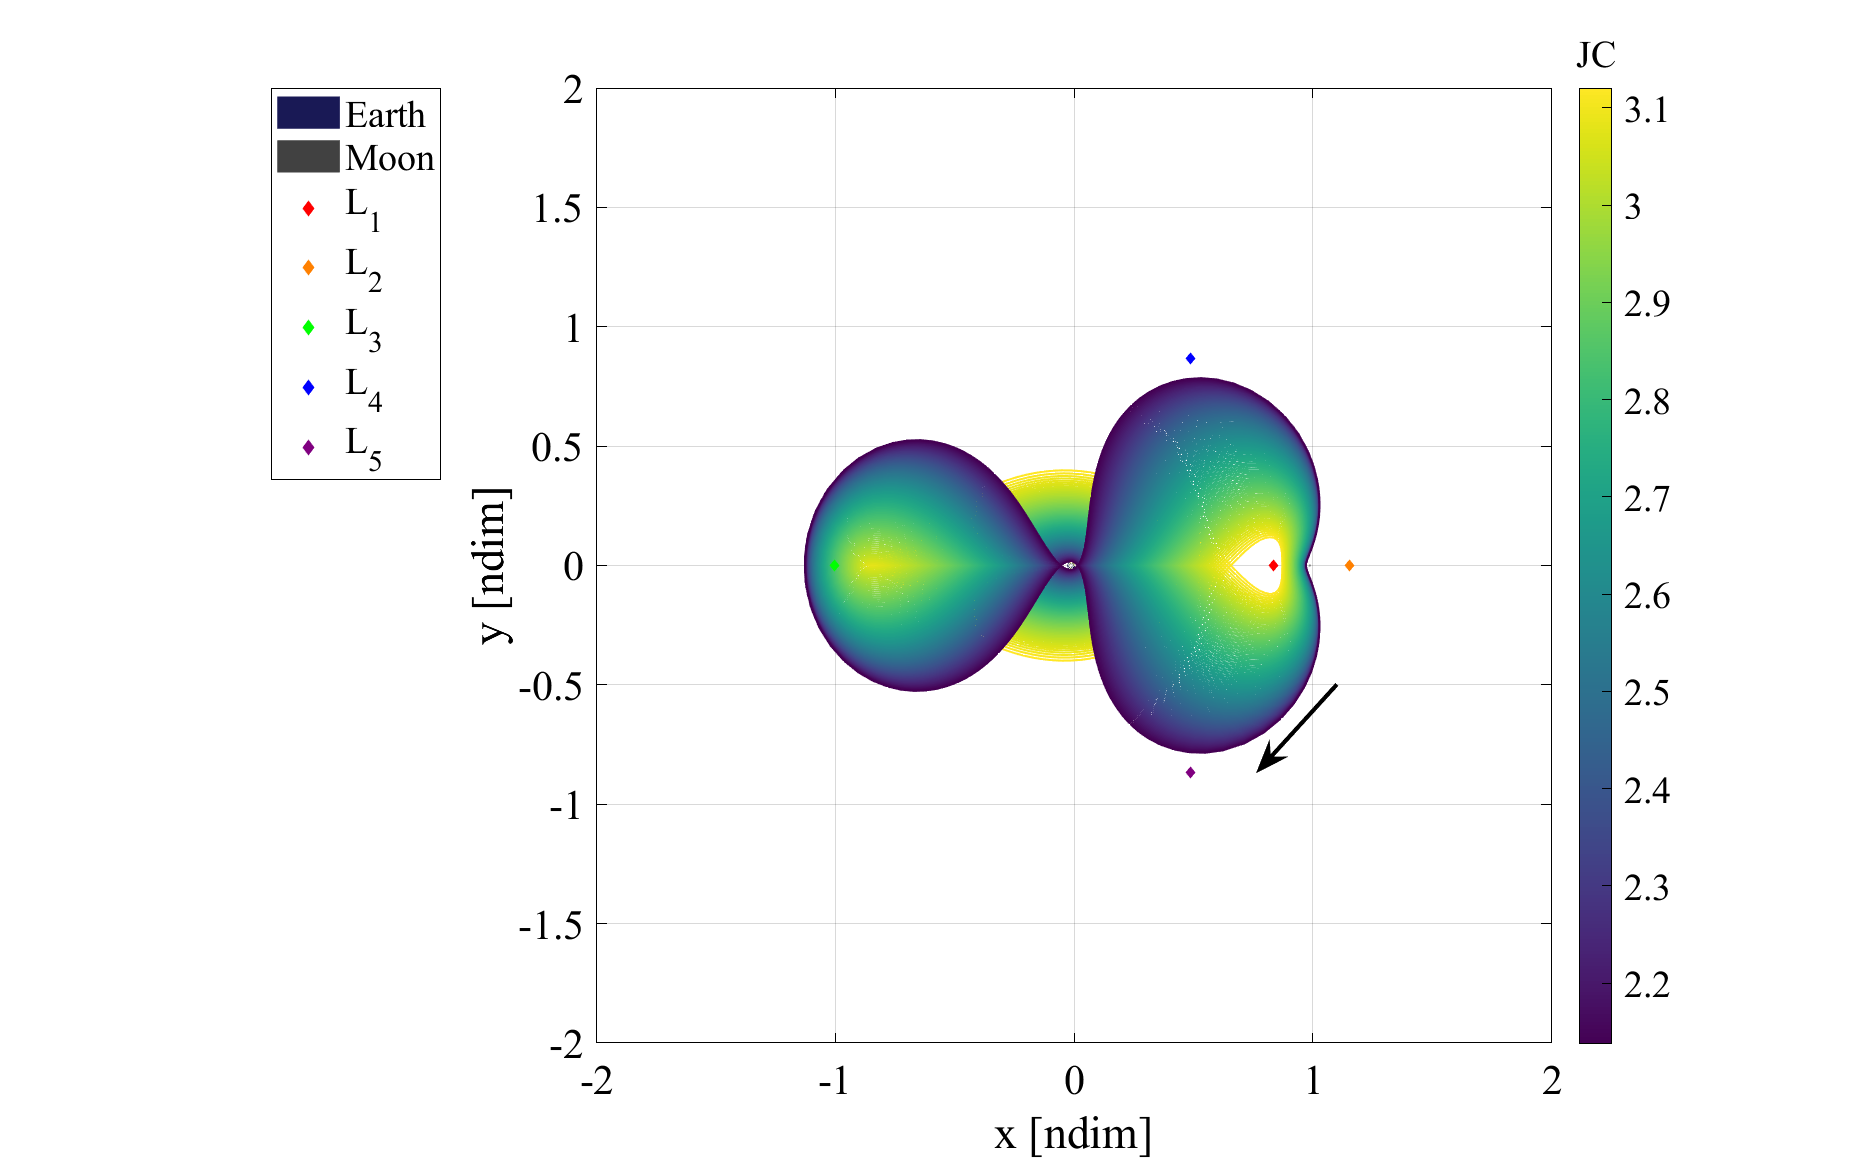
\includegraphics[width=0.9\textwidth]{figures/Resonant2_1aFamily.pdf}
    \caption{Earth-Moon 2:1a resonant orbit family.}
    \label{fig:2_1aResonant}
\end{figure}

\begin{figure}[ht]
    \centering
    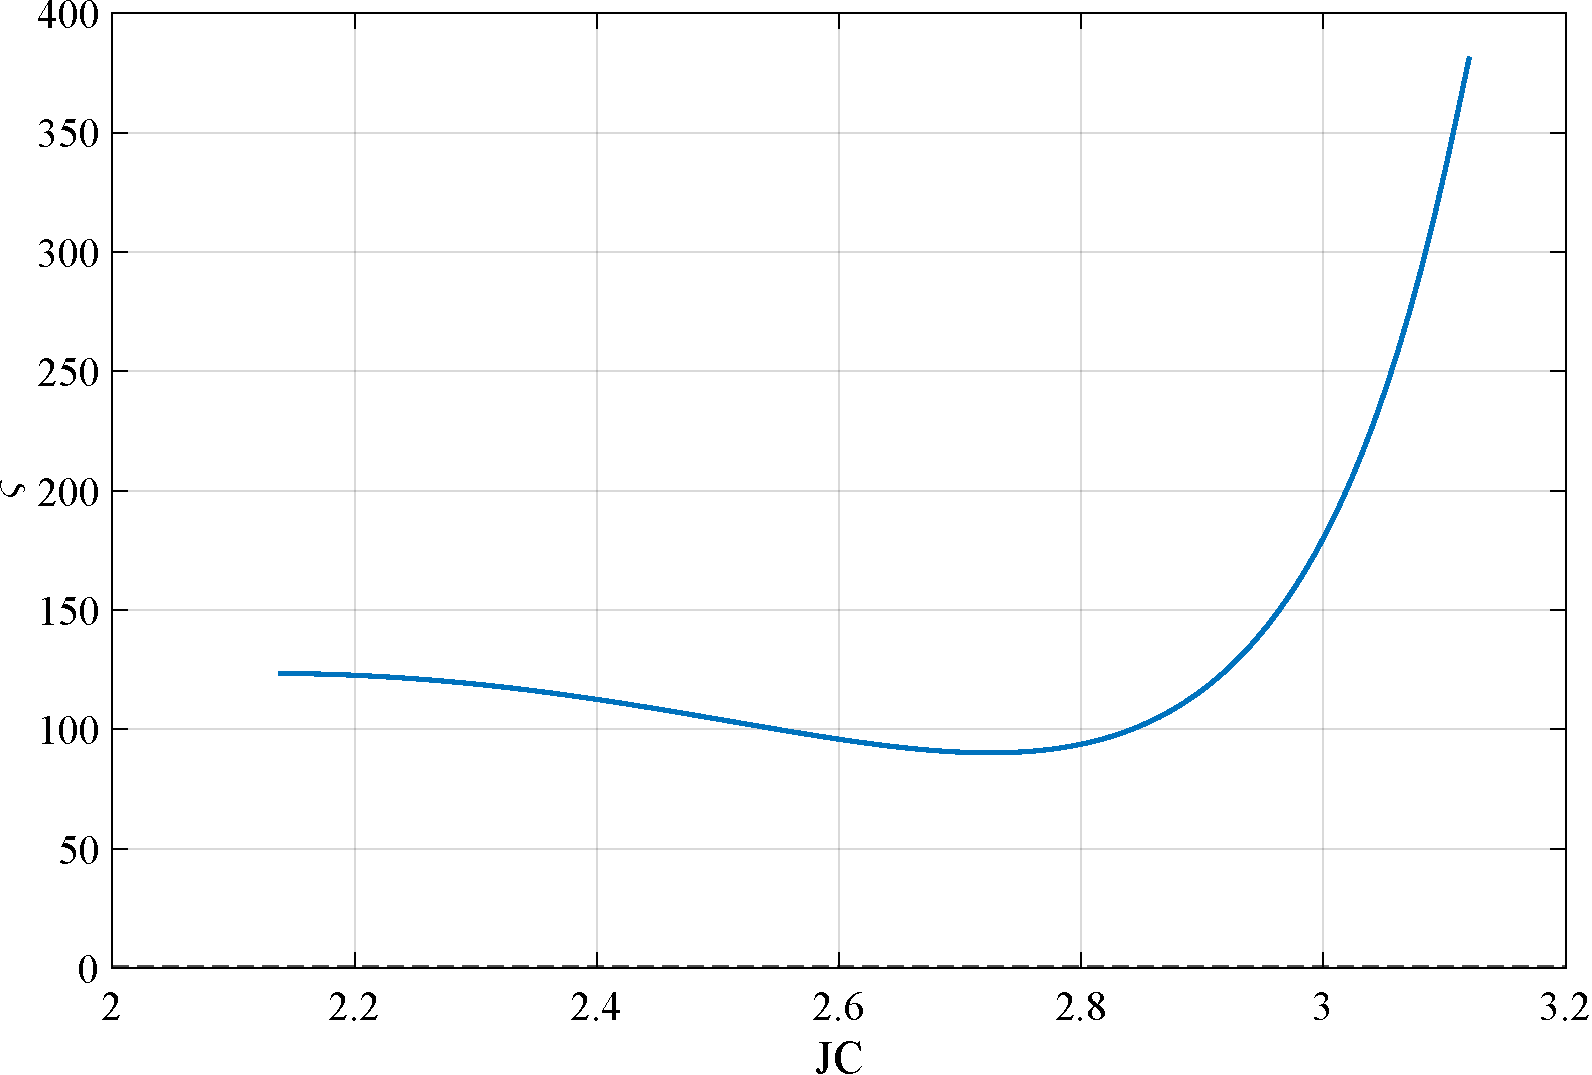
\includegraphics[width=0.5\textwidth]{figures/Resonant2_1aStability.pdf}
    \caption{Earth-Moon 2:1a resonant orbit family stability index evolution.}
    \label{fig:2_1aResonantStability}
\end{figure}

\subsubsection{Converged 3:4 Resonant Orbit Family}
Another unstable family is the 3:4 resonant orbits, shown in \cref{fig:3_4Resonant}. These orbits
go around the Earth three times for every time the Moon goes around. Their stability indices are
given in \cref{fig:3_4ResonantStability}.

\begin{figure}[ht]
    \centering
    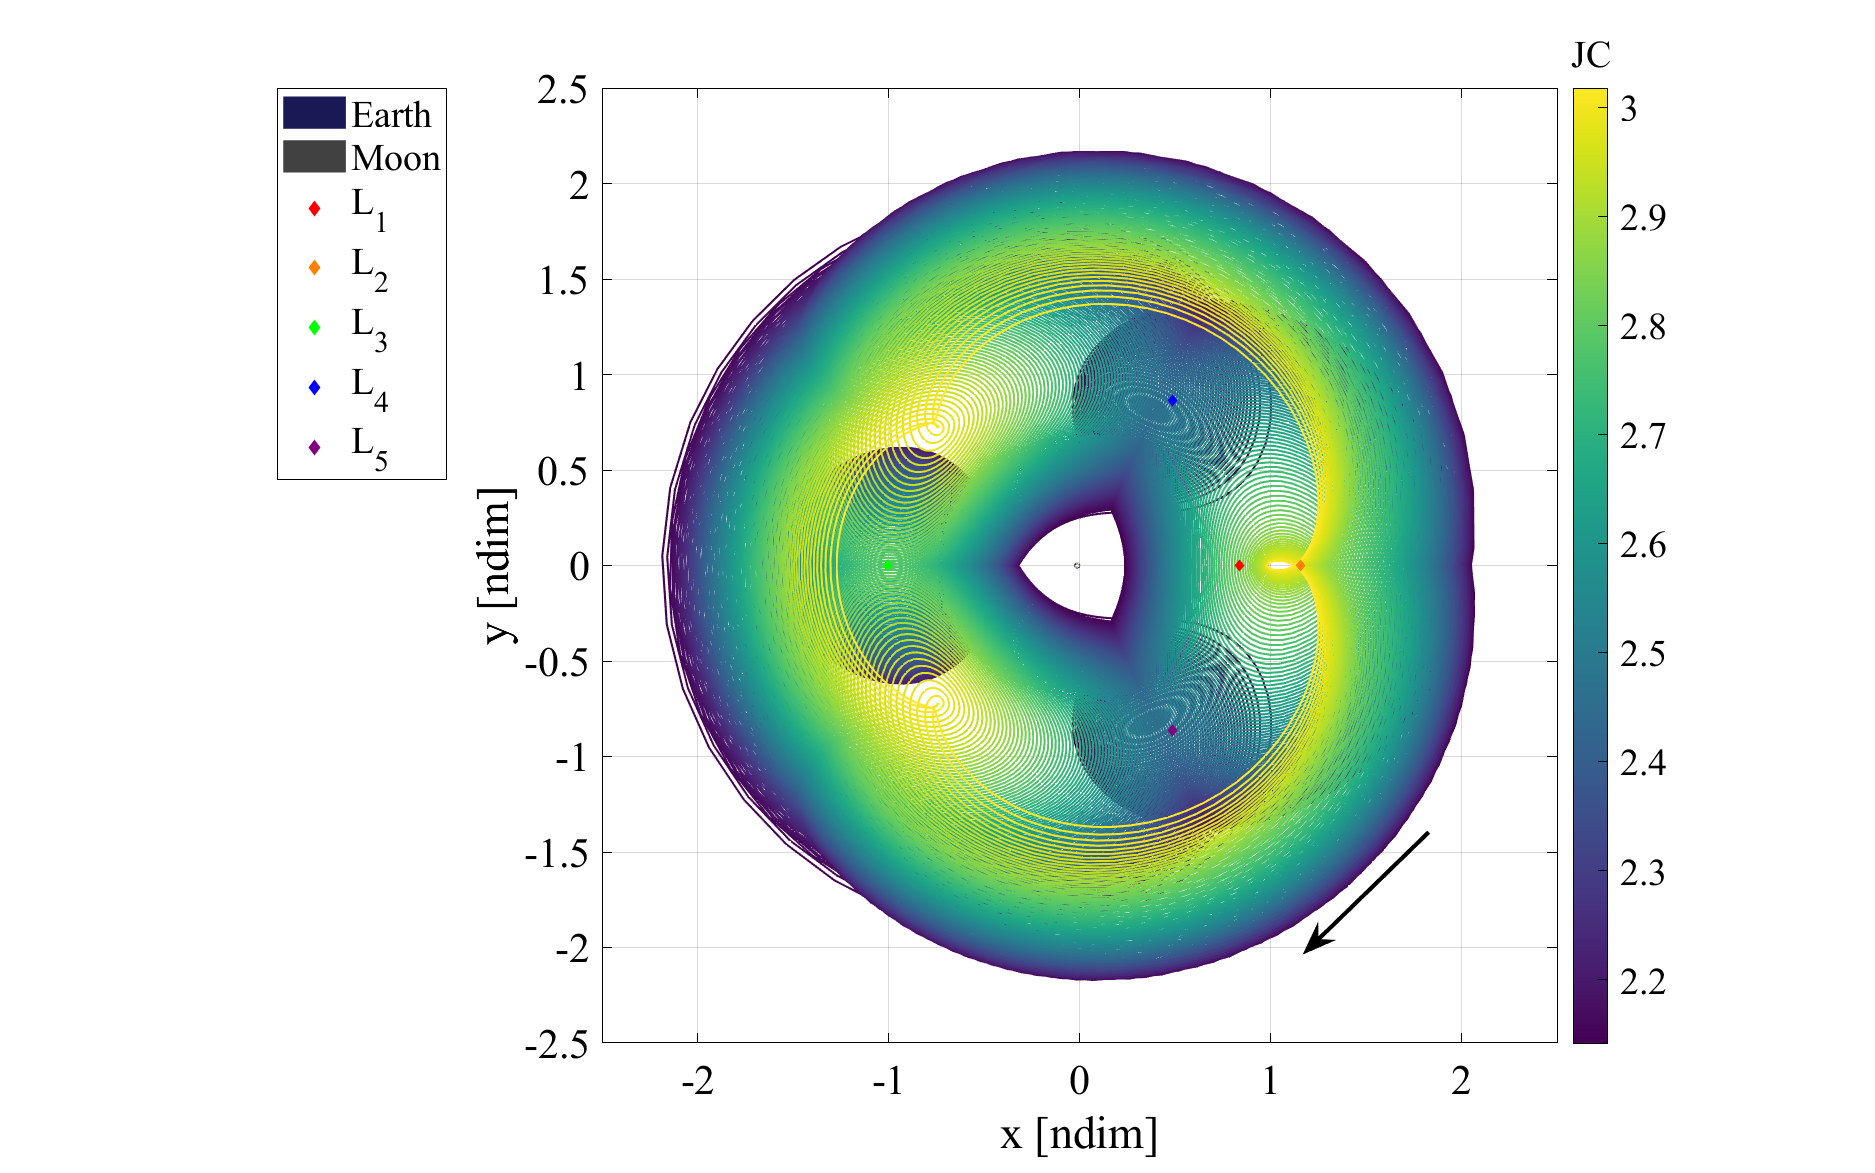
\includegraphics[width=0.9\textwidth]{figures/Resonant3_4Family.pdf}
    \caption{Earth-Moon 3:4 resonant orbit family.}
    \label{fig:3_4Resonant}
\end{figure}

\begin{figure}[ht]
    \centering
    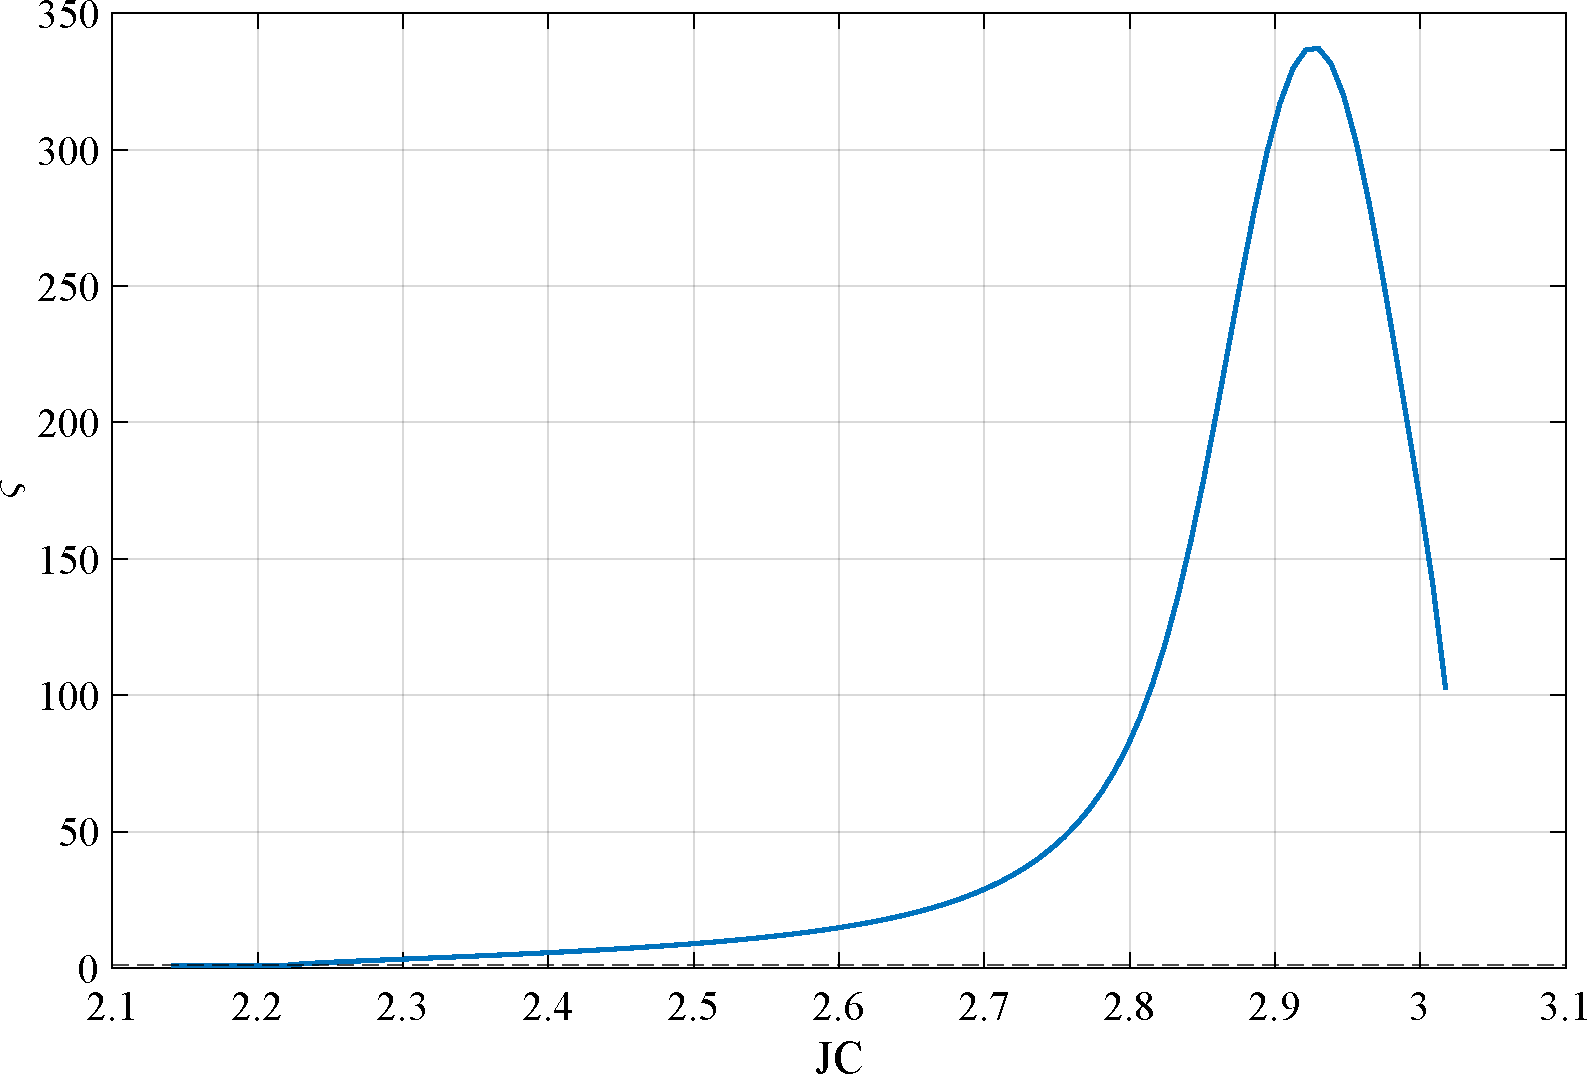
\includegraphics[width=0.5\textwidth]{figures/Resonant3_4Stability.pdf}
    \caption{Earth-Moon 3:4 resonant orbit family stability index evolution.}
    \label{fig:3_4ResonantStability}
\end{figure}

\section{Invariant Manifolds}
Dynamically unstable periodic orbits in the CR3BP have useful structures called invariant manifolds
that represent the local flow near the orbit. With applications for transfer design, trajectories
along these manifold surfaces can be used to arrive at or depart from the periodic orbit
ballistically. Perko provides the following theorem for stable/unstable manifolds for periodic
orbits\cite{Perko:1991}:
\begin{quote}
    Let $f\in C^{1}(E)$ where E is an open subset of $R^{n}$ containing a periodic orbit,
    \begin{equation}
        \Gamma:\xbar=\gamma(t),
    \end{equation}
    of $\xbardot=f(\xbar)$ of period $T$. Let $\phi_{t}$ be the flow of $\xbardot=f(\xbar)$ and
    $\gamma(t)=\phi_{t}(\xbar_{0})$. If $k$ of the characteristic exponents of $\gamma(t)$ have
    negative real part where $0\leq k\leq n-1$ and $n-k-1$ of them have positive real part then
    there is a $\delta>0$ such that the stable manifold of $\Gamma$,
    \begin{equation}
        S(\Gamma)=\{\xbar\in N_{\delta}(\Gamma)|d(\phi_{t}(\xbar),\Gamma)\rightarrow0\text{ as }t\rightarrow\infty\text{ and }\phi_{t}(\xbar)\in N_{\delta}(\Gamma)\text{ for }t\geq0\},
    \end{equation}
    is a $(k+1)$-dimensional, differentiable manifold which is positively invariant under the flow
    $\phi_{t}$ and the unstable manifold of $\Gamma$,
    \begin{equation}
        U(\Gamma)=\{\xbar\in N_{\delta}(\Gamma)|d(\phi_{t}(\xbar),\Gamma)\rightarrow0\text{ as }t\rightarrow-\infty\text{ and }\phi_{t}(\xbar)\in N_{\delta}(\Gamma)\text{ for }t\leq0\},
    \end{equation}
    is an $(n-k)$-dimensional, differentiable manifold which is negatively invariant under the flow
    $\phi_{t}$. Furthermore, the stable and unstable manifolds of $\Gamma$ intersect transversally
    in $\Gamma$.
\end{quote}
In layman's terms, if a periodic orbit is unstable (has eigenvalues greater than and lesser than
$1$), then stable/unstable manifold surfaces exist that approach/leave the orbit asymptotically in
forward time.

Since these manifold structures asymptotically depart the orbit structure, no deterministic
maneuver is required to transfer onto them. However, a consequence of this is that it is not
possible to identify the exact location along the orbit from where a manifold trajectory departs.
Therefore, a numerical process is necessary to approximate the stable/unstable subspace of the
orbit to determine an appropriate initial condition for an arc along the manifold surface.

Near the periodic orbit, the manifolds are tangent to their corresponding eigenspaces of the orbit.
For a selected point on the periodic orbit:
\begin{equation}
    \nubar(t_{0}+t)=\Phi(t_{0}+t,t_{0})\nubar(t_{0}),
    \label{eq:eigenvector}
\end{equation}
where $\nubar(t_{0})$ is the eigenvector at the initial condition corresponding to the stable or
unstable eigenvalue of the monodromy matrix. Once the stable/unstable eigenvector at the selected
point has been obtained:
\begin{equation}
    \nubar_{n}=\frac{\nubar}{\sqrt{\nu_{x}^{2}+\nu_{y}^{2}+\nu_{z}^{2}}},
    \label{eq:normeigenvector}
\end{equation}
where $\nu_{x}$ is the $x$-component of the eigenvector and $\nubar_{n}$ is the eigenvector
normalized by the nondimensional distance from the selected point. Using the normalized
stable eigenvector to approximate the initial condition for a stable manifold arc:
\begin{equation}
    \qbar^{S}=\qbar_{\Gamma}\pm d\nubar_{n}^{S},
    \label{eq:stablemanifold}
\end{equation}
where $\qbar_{\Gamma}$ is the state vector at the selected point along the periodic orbit and $d$
is a step-off distance, generally chosen based on the specific CR3BP system. The scaled eigenvector
can be either added to or subtracted from the periodic state as the eigenspace is bi-directional,
creating two half-manifolds for each stability. To compute an initial condition for an unstable
manifold arc, use \cref{eq:eigenvector}-\cref{eq:stablemanifold}, replacing the stable components
for unstable ones. Stable manifold arcs are then propagated backward in time from the initial
condition (arriving at the orbit in forward time) while unstable arcs are propagated forward in
time from their initial condition.

As mentioned, the value for $d$ depends on the CR3BP system in use. This parameter needs to be
sufficiently small to approximate the manifold structure well. However, if $d$ is too small, the
trajectory will take longer than reasonable to arrive at/depart from the orbit since the dynamics
are asymptotic\cite{Kakoi:2015}. \cref{tab:manifoldValues} shows the values of $d$ used for the
systems in this investigation. As some examples of manifold structures, \cref{fig:LyapunovManifold}
and \cref{fig:haloManifold} show the stable and unstable manifolds for a planar Lyapunov orbit and
a spatial halo orbit, respectively, in the Earth-Moon system. Each figure also shows a single
manifold arc overlayed on the full structure for reference. A more thorough explanation of manifold
theory can be found in Perko\cite{Perko:1991}.

\begin{figure}[ht]
    \centering
    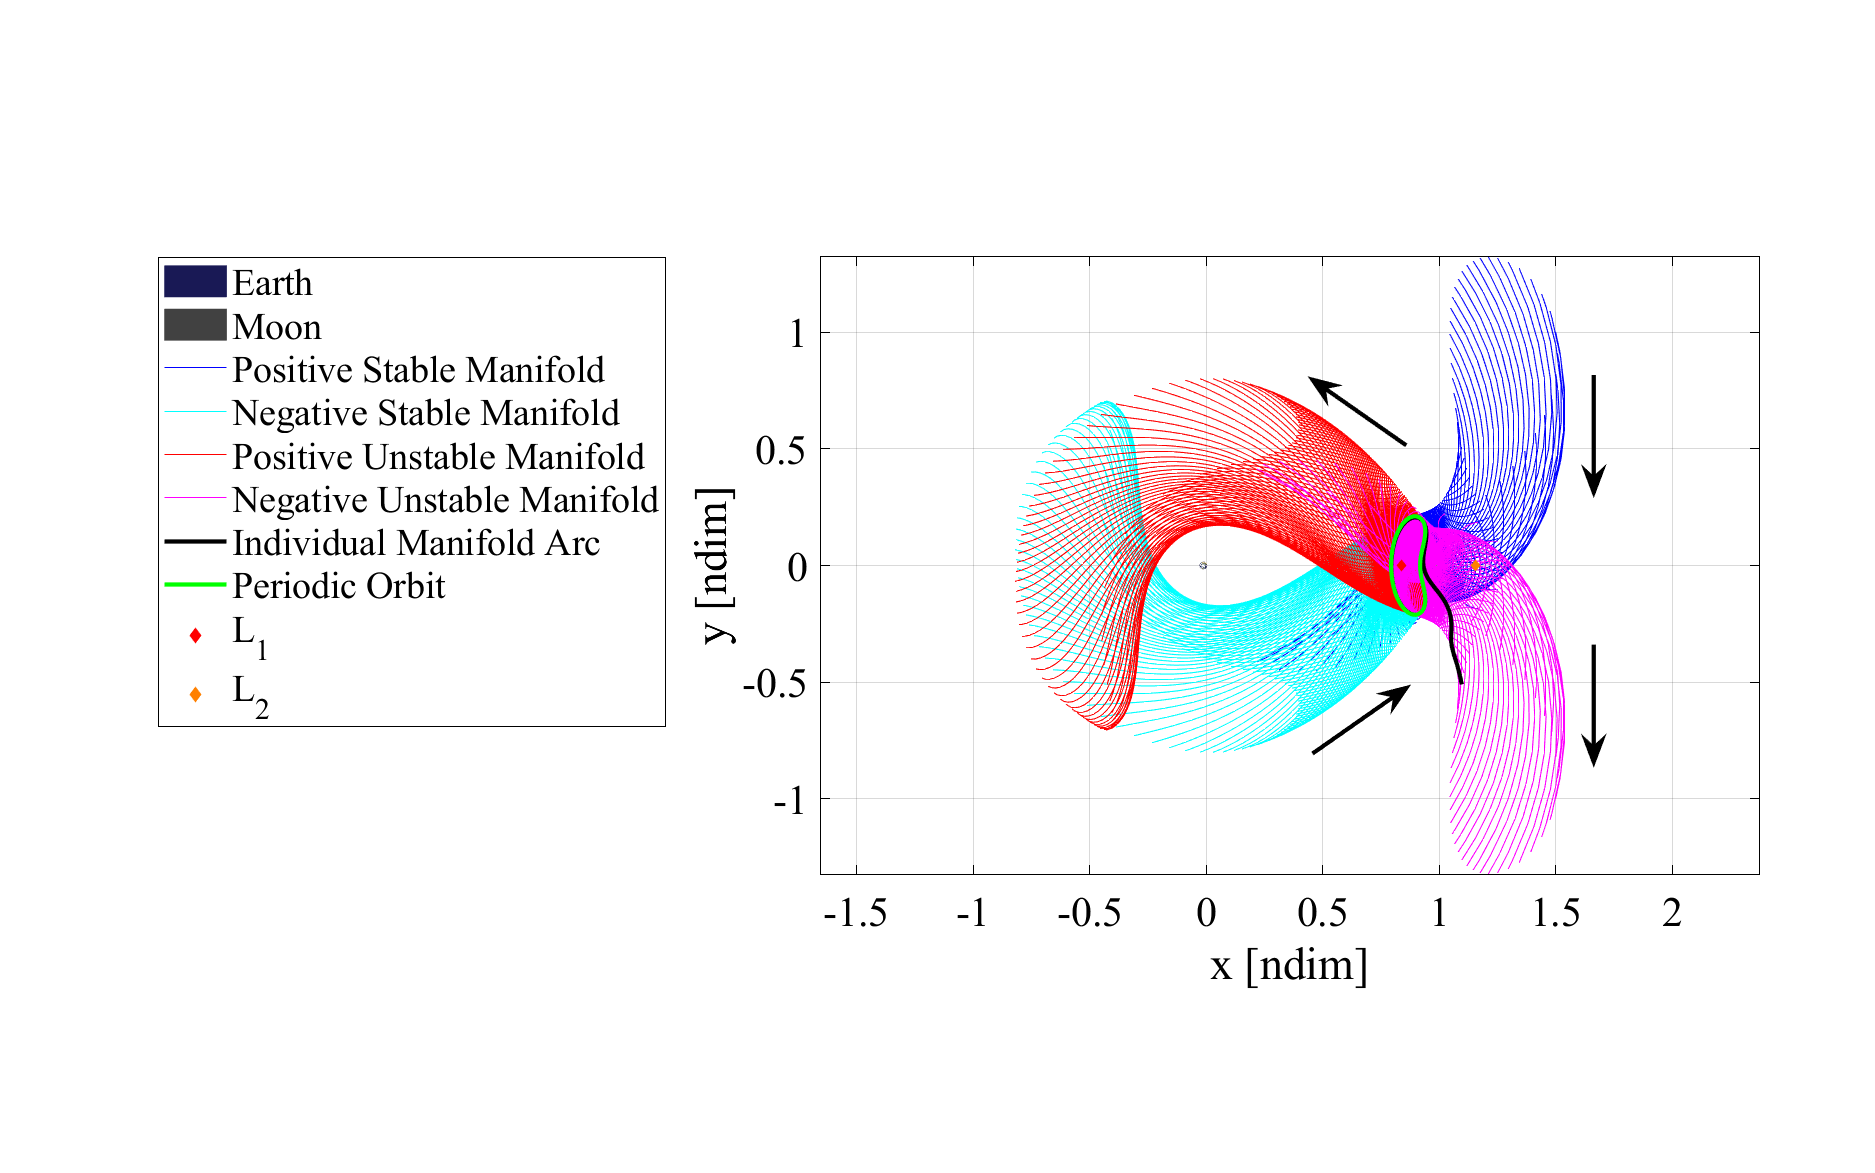
\includegraphics[width=0.9\textwidth]{figures/LyapunovManifold.pdf}
    \caption{Earth-Moon $L_{1}$ Lyapunov Manifolds ($C=3.05$).}
    \label{fig:LyapunovManifold}
\end{figure}

\begin{figure}[ht]
    \centering
    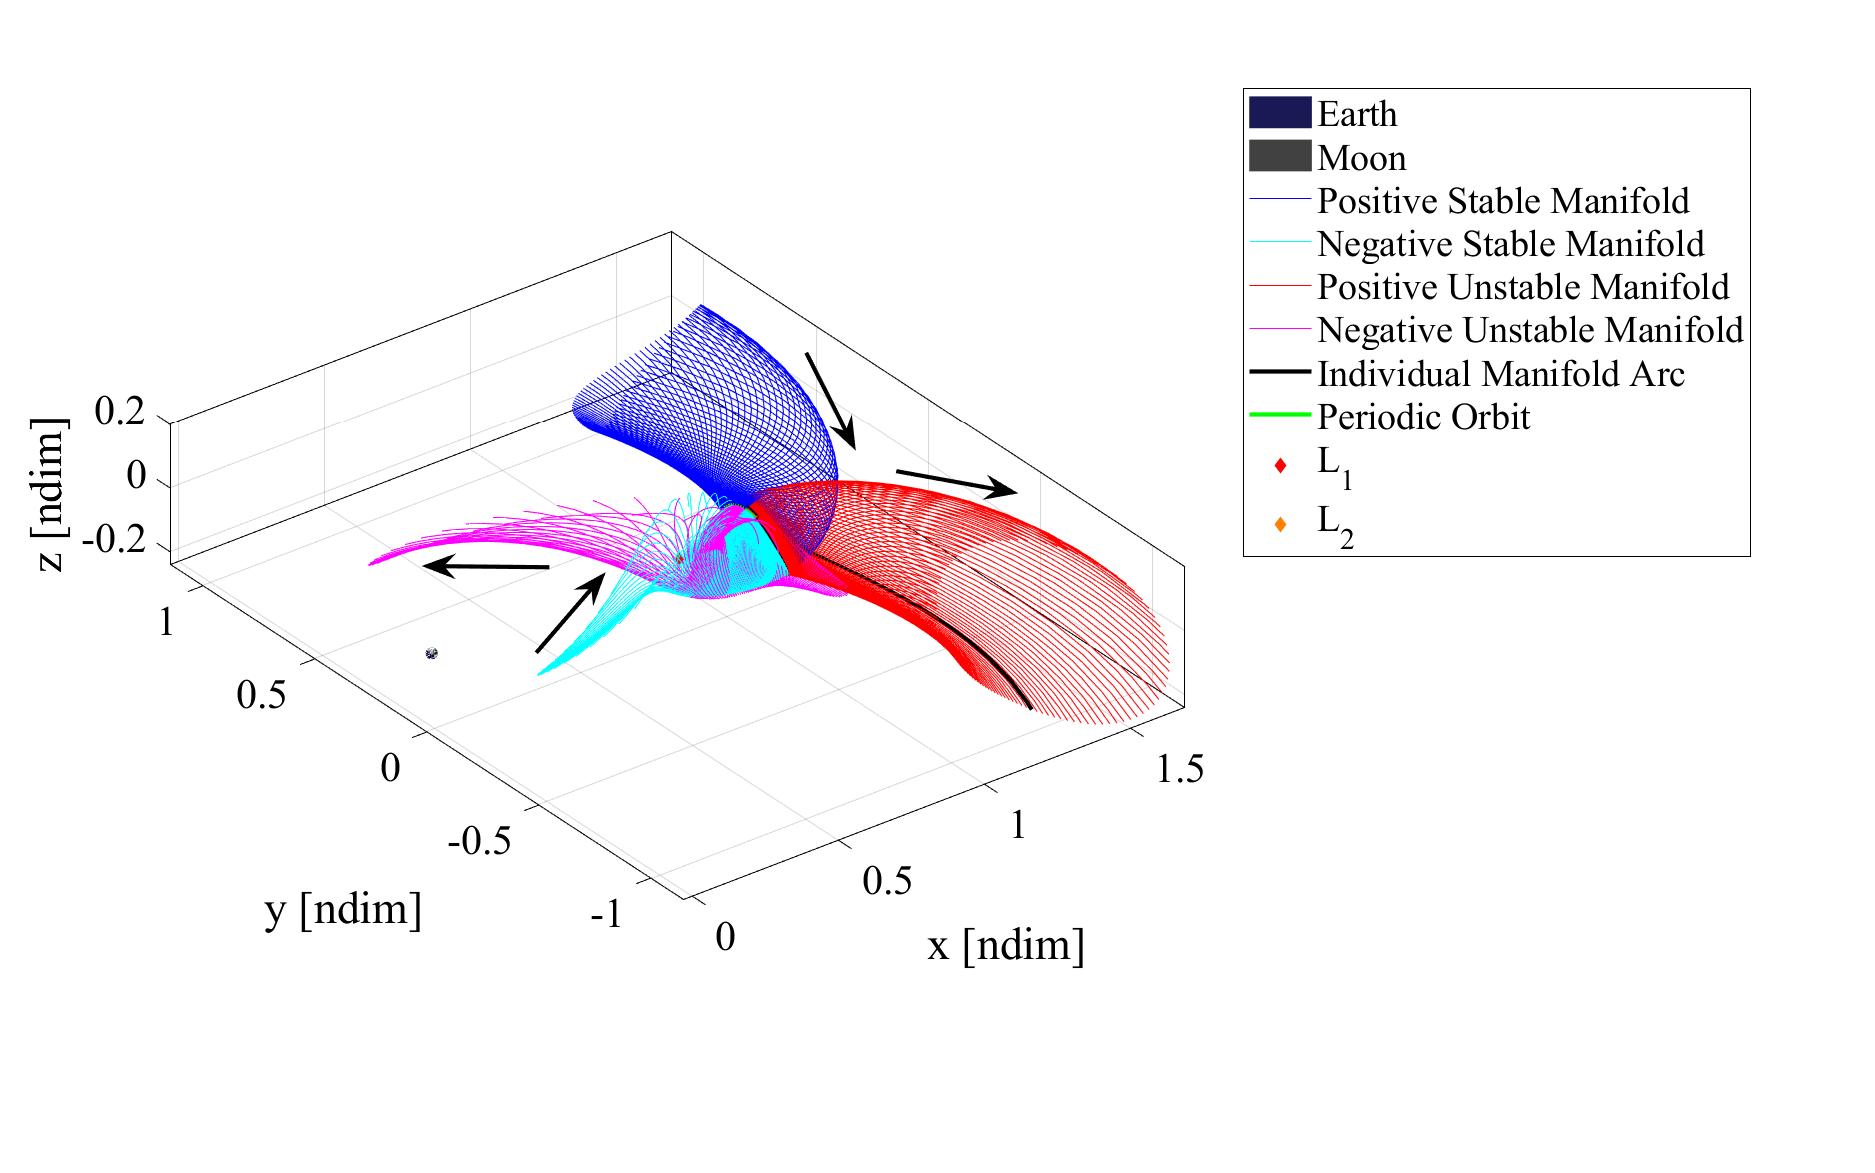
\includegraphics[width=0.9\textwidth]{figures/HaloManifold.pdf}
    \caption{Earth-Moon $L_{2}$ Halo Manifolds ($C=3.08$).}
    \label{fig:haloManifold}
\end{figure}

Since manifolds asymptotically arrive at/depart from their orbit, even with a reasonable step-off
distance, they can take a long time to depart from the orbit vicinity. Under higher-fidelity
dynamics, this period of time would be eliminated from the mission design, so it would be useful to
have a metric to determine when the manifold has departed the orbit vicinity. In this
investigation, the momentum integral, or more specifically the momentum integral difference, is
used to indicate orbit departure:
\begin{equation}
    MI=\int_{t_{0}}^{t}(x\xdot+y\ydot+z\zdot)d\tau,
    \label{eq:momentumintegral}
\end{equation}
where all of the values are nondimensional. Starting from $MI_{0}=0$ at the step-off location, the
momentum integral is calculated for both the orbit and the manifold arc and the difference between
the two values measures the similarity of the two trajectories:
\begin{equation}
    \Delta MI=|MI-MI_{\Gamma}|.
    \label{eq:momentumdifference}
\end{equation}
Once $\Delta MI$ has reached a threshold value (determined for each system), the trajectory is
considered departed from the orbit\cite{Guzzetti:2017}. \cref{tab:manifoldValues} shows the
threshold values chosen for each system in this investigation.

\begin{table}[ht]
    \centering
    \caption{Manifold-related values of relevant CR3BP systems.}
    \begin{tabular}{|c|c|c|}
        \hline
        \textbf{CR3BP System}   &   \boldmath$d$ \textbf{[km]}  &   \boldmath$\Delta MI$    \\  \hline
        Earth-Moon              &   $25$                        &   $1\times10^{-3}$        \\  \hline
        Sun-Earth               &   $1000$                      &   $5\times10^{-5}$        \\  \hline
        Sun-Mars                &   $1000$                      &   $1\times10^{-5}$        \\  \hline
    \end{tabular}
    \label{tab:manifoldValues}
\end{table}

\section{Poincar\'e Maps}\label{sec:PoincareMaps}
Since plots of invariant manifolds in configuration space can be complex and do not display any
velocity information about the trajectories, a different visualization technique is advantageous.
Poincar\'e mapping is an approach that concisely visualizes trajectories by reducing the dimension
of the problem through an intersection surface. These surfaces can be physical, like a plane or
sphere in configuration space, or more abstract, like an apse or velocity map. As initial
conditions are propagated, whenever a trajectory passes through the surface, its crossing is
marked on the Poincare\'e map. A simple example appears in \cref{fig:map}. The mapping technique
provides an intuitive representation of complex trajectory behaviors, aiding in the analysis and
interpretation of manifold dynamics.

\begin{figure}[H]
    \centering
    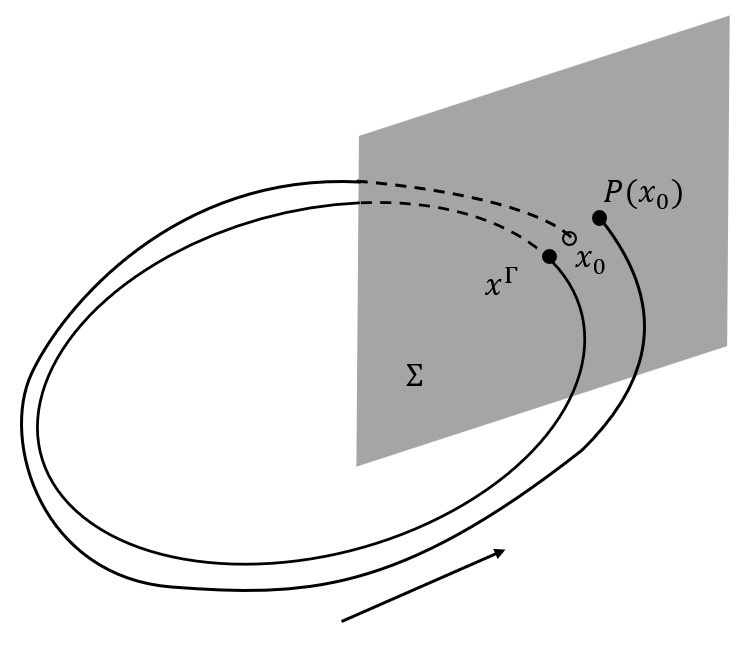
\includegraphics[width=0.5\textwidth]{figures/Map.jpg}
    \caption{Poincar\'e map.}
    \label{fig:map}
\end{figure}

Poincaré mapping provides a powerful method for visualizing and analyzing trajectory behavior by
reducing the dimensionality of the problem through surface intersections. Starting from an initial
condition $x_{0}$ on the intersection surface $\Sigma$, after propagation, the trajectory returns
to the surface at $P(x_{0})$. If the trajectory is precisely periodic, the trajectory returns to
the same point, $x^{\Gamma}$. The Poincar\'e map then is the 2-dimensional representation of the
surface, displaying only the trajectory crossings. Note that the axes of the map need not be
position components but could also be velocity, energy, etc. Similar mappings are employed in this
investigation to more efficiently analyze and compare different trajectories.


\chapter{CISLUNAR-MARS TRAJECTORY CONSTRUCTION}

Many of the techniques introduced in the previous chapter are used in this investigation to design
end-to-end transfers between orbits in the Earth-Moon and Sun-Mars CR3BP systems. Two categories of
transfers are designed and compared: trajectories that include an intermediate Sun-Earth staging
halo orbit and those that do not. For the transfers utilizing a staging orbit, a strategy is
adapted from Kakoi to compute near-ballistic transfer solutions between Earth-Moon unstable orbits
and Sun-Earth halos via invariant manifolds\cite{Kakoi:2015}. Both sets of transfers then use a
variation of the moon-to-moon analytical transfer methodology developed by Canales to bridge the
gap between the Sun-Earth trajectories (either Sun-Earth manifolds or Earth-Moon manifolds
propagated under Sun-Earth dynamics) and the Sun-Mars manifolds\cite{Canales:2021b}. Note that this
transfer design process may not result in optimized interplanertary transfers, but instead provides
families of low-energy solutions to facilitate the comparison between cislunar departure orbits. As
a baseline comparison metric, Keplerian Lambert arcs are also introduced here to represent the
current standard for direct Earth-Mars transfers.

\section{Near-Ballistic Transfers between the Earth-Moon and Sun-Earth Systems}

\section{The Moon-to-Moon Analytical Transfer Method}
The MMAT method was created to design tours between the moons of a planet such as Jupiter or
Saturn. However, Canales also showed that it could similarly be used for interplanetary transfers
by treating the planets as "moons" of the Sun. He provides detailed derivations, analyses, and
examples of the basic MMAT strategy, as well as some extensions relevant to this
investigation\cite{Canales:2021a,Canales:2021b,Canales:2022}. More specifically, the end-to-end
cislunar-Mars transfer methodology presented here uses a distant, two-burn MMAT with a plane
change. This accounts for bridging the gap between manifolds of Sun-planet CR3BP systems and the
true orbital plane inclinations of the planets.

\subsection{Methodology}
First, a departure and an arrival CR3BP arc are needed. In this investigation, the departure CR3BP
arc is either a Sun-Earth halo orbit unstable manifold trajectory or an Earth-Moon orbit unstable
manifold arc propagated with the Sun-Earth dynamics, depending on the transfer category. Either the
departure epoch or the chosen manifold arc are varied to determine the departure CR3BP arc
respectively. The arrival CR3BP arc is a Sun-Mars halo orbit stable manifold trajectory. Since an
interplanetary transfer from Earth to Mars is an outward journey, to minimize the $\Delta v$ of the
MMAT transfer, the Sun-Mars stable manifold with the smallest periapsis (relative to the Sun) is
used\cite{Canales:2021b}. (For an inward journey, say to Venus, the manifold with the largest
apoapsis is chosen.) This minimizes the Keplerian angular momentum and energy difference between
the departure and arrival CR3BP arcs.

These arcs are propagated under the CR3BP dynamics until they reach a specified distance from their
smaller primary (Earth or Mars), their sphere of influence. Various definitions exist, but for the
MMAT method, the SoI radius is defined as the distance for which the ratio of the gravitational
accelerations of the two primaries $d_{SoI}$ is equal to a chosen small quantity (see
\cref{eq:patchedSoI})\cite{Canales:2021b}. To ensure that the SoI encompasses most of the Lyapunov
family but also accurately represents when that body's gravitational effects can be neglected, the
values of $d_{SoI}$ in \cref{tab:SoI} are chosen, resulting in their corresponding radii. Canales
provides more details on selecting of appropriate values for $d_{SoI}$\cite{Canales:2021b}.

\begin{table}[ht]
    \centering
    \caption{MMAT sphere of influence radii of relevant CR3BP systems.}
    \begin{tabular}{|c|c|c|}
        \hline
        \textbf{CR3BP System}   &   \boldmath$d_{SoI}$  &   \boldmath$r_{SoI}$  \\  \hline
        Sun-Earth               &   $2.5\times10^{-4}$  &   $0.09877$           \\  \hline
        Sun-Mars                &   $1\times10^{-4}$    &   $0.05375$           \\  \hline
    \end{tabular}
    \label{tab:SoI}
\end{table}

Once the CR3BP arc has reached the edge of the SoI, it can be treated as a 2BP trajectory with the
Sun as its focus (refer to the patched 2BP-CR3BP model introduced in Section 2.4.1). The
barycentric rotating frame state that intersects the SoI is transformed to a heliocentric Ecliptic
J2000 frame state using the procedure outlined in Section 2.5.2. The resulting state now defines a
Keplerian heliocentric ellipse in the instantaneous plane of motion of the trajectory at the SoI,
the path for either the departure or arrival conic arc.
\cref{eq:inclination}-\cref{eq:radialvelocity} can be used to retrieve the equivalent Keplerian
orbital elements.

In the distant, two-burn MMAT strategy, the first maneuver is placed at the periapsis of the
departure conic. Given that the true anomaly $\theta=0$ at periapsis,
\cref{eq:eccentricanomaly}-\cref{eq:velocityvector} are used to compute the inertial state at
periapsis while \cref{eq:meananomaly} and \cref{eq:Keplersequation} are used to compute the
time-of-flight along the departure conic:
\begin{equation}
    TOF_{d}=\mathbb{P}_{d}-(t-t_{p}),
    \label{eq:departureTOF}
\end{equation}
where $\mathbb{P}_{d}$ is the period of the departure conic and $(t-t_{p})$ is the time since
periapsis of the SoI state.

As mentioned previously, a bridge arc is needed to connect the departure and arrival conic arcs,
with a maneuver at both ends. The distant, two-burn MMAT bridge arc has the same periapsis radius
as the departure conic arc and the same apoapsis as the arrival conic arc. These values form a
bridge ratio which can then be used to compute the semimajor axis and eccentricity of the bridge
conic:
\begin{equation}
    \mathcal{P}_{b}=\frac{r_{p_{b}}}{r_{a_{b}}}=\frac{1-e_{b}}{1+e_{b}},
    \label{eq:bridgeratio}
\end{equation}
\begin{equation}
    e_{b}=\frac{1-\mathcal{P}_{b}}{1+\mathcal{P}_{b}},
    \label{eq:bridgeeccentricity}
\end{equation}
\begin{equation}
    a_{b}=\frac{r_{p_{b}}}{1-e_{b}}.
    \label{eq:bridgesemimajoraxis}
\end{equation}
The remaining three angles of the bridge conic ($i$, $\Omega$, $\omega$) are identical to those of
the departure conic, implying that the bridge arc lies in the same plane as the departure conic
arc. Since only the semimajor axis and eccentricity change between the departure and bridge conics,
this first maneuver is tangential to the motion (only changing the energy) at periapsis and can be
calculated by the difference in the velocity states at periapsis.

The non-coplanar MMAT methodology revolves around the following analytical constraint derived by
Canales\cite{Canales:2021b}:
\begin{quote}
    As long as the geometrical properties of two conics located in different planes fulfill the
    inequality constraint represented by
    \begin{equation}
        a_{a}(1-e_{a})\leq\frac{a_{b}(1-e_{b}^{2})}{1+e_{b}\cos(\theta_{b_{int}}+n\pi)}\leq a_{a}(1+e_{a}),\text{ being }n=0,1,
        \label{eq:MMAT}
    \end{equation}
    either one of the two conics can be reoriented such that they intersect in space. Consequently,
    the ideal phase of the arrival [planet] at arrival, $\theta_{5_{Mars}}$, for the moon-to-moon
    transfer to occur is obtained considering that the departure epoch, $\theta_{0_{Earth}}$, is
    fixed.
\end{quote}
In this constraint, $\theta_{5_{Mars}}$ and $\theta_{0_{Earth}}$ correspond to $T_{0}$ and $T_{5}$
in \cref{fig:MMAT}. This figure is a schematic of the distant, two-burn MMAT transfer with a plane
change, where the departure and bridge conics are on the same plane but the arrival conic is not.
With the semimajor axes and eccentricities of the bridge and arrival arcs already determined, the
only value still needed for \cref{eq:MMAT} is $\theta_{b_{int}}$, the bridge conic true anomaly at
the bridge-arrival conic intersection location ($T_{3}$ in \cref{fig:MMAT}):
\begin{equation}
    \theta_{b_{int}}=u_{b}-\omega_{b},
    \label{eq:bridgeintersect}
\end{equation}
\begin{equation}
    \sin u_{b}=\frac{\sin(\pi-i_{a})\sin\Delta\Omega}{\sin\psi},
    \label{eq:bridgesinu}
\end{equation}
\begin{equation}
    \cos u_{b}=\frac{\frac{\sin i_{a}\cos\Delta\Omega}{\cos i_{b}}-\cos\psi\tan i_{b}}{\sin\psi},
    \label{eq:bridgecosu}
\end{equation}
\begin{equation}
    \cos\psi=\cos i_{a}\cos i_{b}+\sin i_{a}\sin i_{b}\cos\Delta\Omega,
\end{equation}
where $\Delta\Omega=\Omega_{a}-\Omega_{b}$. Note that the value of $n$ used to satisfy the
inequality defines the orientation of the bridging conic and will be used later to properly orient
the arrival conic. The center of the inequality in \cref{eq:MMAT} is the intersection distance from
the Sun:
\begin{equation}
    r_{int}=\frac{a_{b}(1-e_{b}^{2})}{1+e_{b}\cos(\theta_{b_{int}}+n\pi)}=\frac{a_{a}(1-e_{a}^{2})}{1+e_{a}\cos(\theta_{a_{int}}+o\pi)}, \text{ being }o=0,1.
    \label{eq:intersect}
\end{equation}
Unfortunately, if the arrival conic arc is not in the same plane as the orbital plane of the
arrival planet, $i_{a}$ and $\Omega_{a}$ cannot be determined prior to the MMAT phasing (yet to
come). As a result, the arrival phasing needs to be iteratively targeted, making this approach now
only semi-analytical. For an initial guess to check the MMAT constraint in \cref{eq:MMAT}, the
inclination and RAAN of the arrival planet's orbital plane are used.

\begin{figure}[ht]
    \centering
    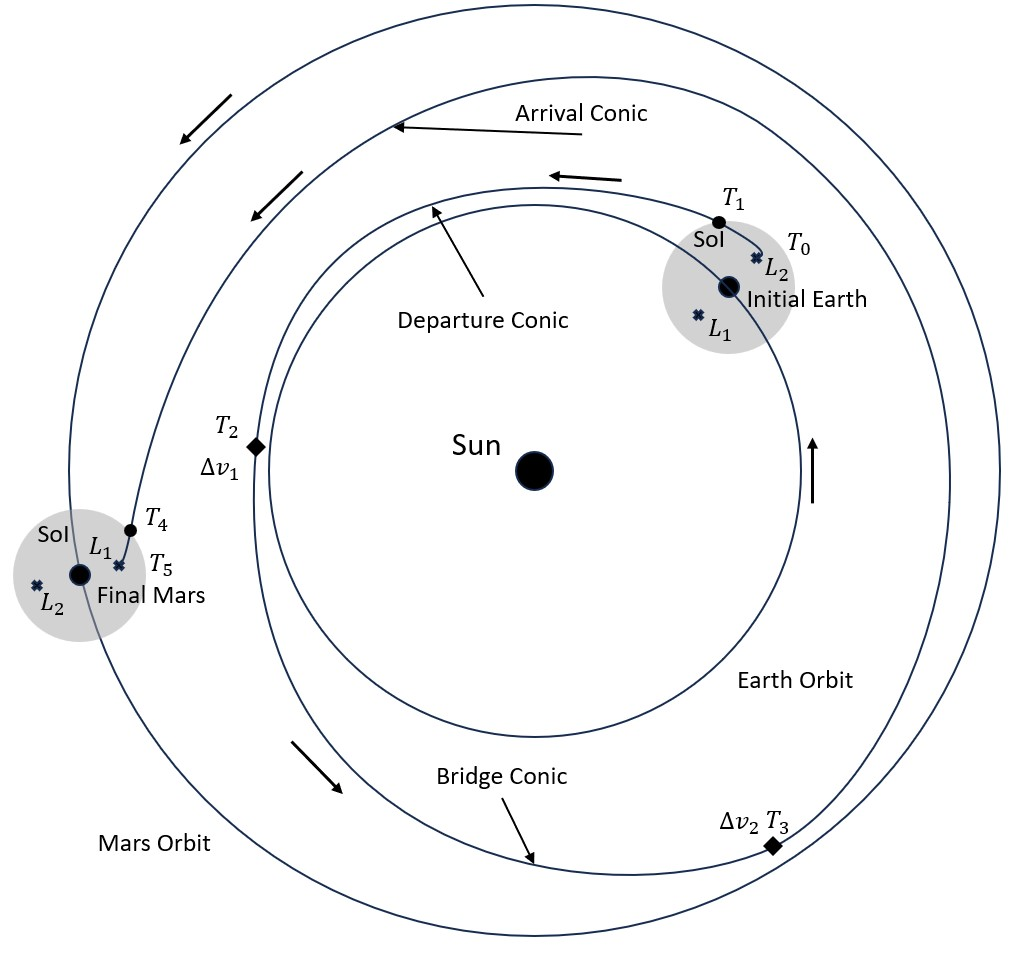
\includegraphics[width=0.75\textwidth]{figures/MMAT.jpg}
    \caption{Representation of the distant, two-burn MMAT with a plane change (adapted from Canales\cite{Canales:2021b}).}
    \label{fig:MMAT}
\end{figure}

The arrival conic true anomaly at the intersection is computed similarly from $r_{int}$, with the
caveat that it is dependent on the arrival phasing and needs to be targeted:
\begin{equation}
    \theta_{a_{int}}=2\pi o+(-1)^{o}\arccos(\frac{\frac{a_{a}(1-e_{a}^{2})}{r_{int}}-1}{e_{a}}),\text{ being }o=0,1.
    \label{eq:arrivalintersect}
\end{equation}
For every feasible $\theta_{b_{int}}$, there are then two possible phasing solutions
($\theta_{a_{int}}$) that correspond to the two arrival ellipse orientations ($\omega_{a}$) that
intersect the bridge ellipse at the line of nodes. A schematic representing these two orientations
is shown in \cref{fig:orientation}, where the dashed part of the ellipses are under the $XY$-plane
and the arrows show the direction of motion along each ellipse. The angles for the orientation are
calculated similarly to before:
\begin{equation}
    \omega_{a}=u_{a}-(\theta_{a_{int}}+n\pi),
    \label{eq:arrivalperiapse}
\end{equation}
\begin{equation}
    \sin u_{a}=\frac{\sin i_{b}\sin\Delta\Omega}{\sin\psi},
    \label{eq:arrivalsinu}
\end{equation}
\begin{equation}
    \cos u_{a}=\cos\Delta\Omega\cos u_{b}+\sin\Delta\Omega\sin u_{b}\cos i_{b}.
    \label{eq:arrivalcosu}
\end{equation}
\cref{eq:arrivalperiapse} is dependent on the orientation of the arrival CR3BP arc, which in turn
depends on a properly phased arrival. Therefore, to solve for the proper phasing and orientation,
an iterative Newton-Raphson differential corrections scheme is applied:
\begin{equation}
    \Xbar=\begin{bmatrix}   \theta_{b_{int}}    &   \theta_{4_{Mars}}   &   \theta_{a_{int}}    \end{bmatrix}^{T},
    \label{eq:MMATfreevar}
\end{equation}
\begin{equation}
    \Fbar(\Xbar)=\rbar_{a}-\rbar_{b},
    \label{eq:MMATconst}
\end{equation}
where $\theta_{4_{Mars}}$ corresponds to Mars' true anomaly when the trajectory intersects the Mars
SoI. For an initial guess:
\begin{equation}
    \theta_{4_{Mars}}=\arctan(\cos i_{Mars}\tan\Omega_{Mars})+\omega_{a}+\theta_{a}-(\Omega_{Mars}+\omega_{Mars}+\theta_{Mars_{J2000}})-\arctan(\frac{y_{4}}{|x_{4}|}),
    \label{eq:arrivalepoch}
\end{equation}
where $\theta_{a}$ is the true anomaly of the arrival conic at the SoI intersection,
$\theta_{Mars_{J2000}}$ is Mars' true anomaly when the J2000 frame is defined, and $x_{4}$ and
$y_{4}$ are the rotating frame coordinates of the trajectory at the SoI intersection. For this
targeting problem, the $DF$ Jacobian matrix is determined using the central difference method (see
Section 3.1.3).

\begin{figure}[ht]
    \centering
    \includegraphics[width=0.9\textwidth]{figures/orientation.jpg}
    \caption{Representation of the two feasible arrival ellipse orientations. The top images are $XY$-plane views while the bottom are $XZ$-plane views.}
    \label{fig:orientation}
\end{figure}

Once $\Xbar$ has been solved, these true anomaly angles can be used to compute the Cartesian
states at each location and the times-of-flight of each segment as was done for the departure conic
arc. At the intersection of the bridge and arrival conics, the second maneuver applies an
inclination change on top of the energy change so it is not tangential like the first burn. This
$\Delta v$ can still be calculated from the difference in the velocity states at the intersection.

The MMAT transfer between the Sun-Earth CR3BP arc and the Sun-Mars CR3BP arc is now completed. The
trajectory should be position-continuous throughout, with a maneuver at the beginning and end of
the bridge arc to account for the velocity discontinuities. For every feasible $\theta_{b_{int}}$,
there will be two corresponding $\theta_{a_{int}}$ that provide transfers. These two solutions will
have different maneuver costs and times-of-flight. By continuing in the departure epoch or the
chosen manifold arc as discussed, a family of MMAT solutions can be obtained and compared.

\subsection{Example}
What follows is an example MMAT family between a Sun-Earth CR3BP northern halo orbit at a Jacobi
constant of $3.0008189$ and a Sun-Mars CR3BP northern halo orbit at a Jacobi constant of
$3.0001857$. Each transfer in the family starts at a different initial epoch, each day in an Earth
year. These initial epochs correspond to $\theta_{0_{Earth}}$ values (which spans
0\textdegree-360\textdegree in a year). All of the trajectories use the same departure CR3BP arc,
which is the Sun-Earth halo unstable manifold with the largest apoapsis, shown in
\cref{fig:MMATSE}. Similarly, all of the trajectories use the same Sun-Mars halo stable manifold
with the smallest periapsis as the arrival CR3BP arc, shown in \cref{fig:MMATSM}. In both figures,
the trajectory is propagated and displayed to the edge of the sphere of influence. In between, the
departure and arrival conic arcs are determined by the osculating Keplerian orbital elements when
the manifolds reach their respective SoIs and the bridge conic arc joins them as described above.

\begin{figure}[ht]
    \centering
    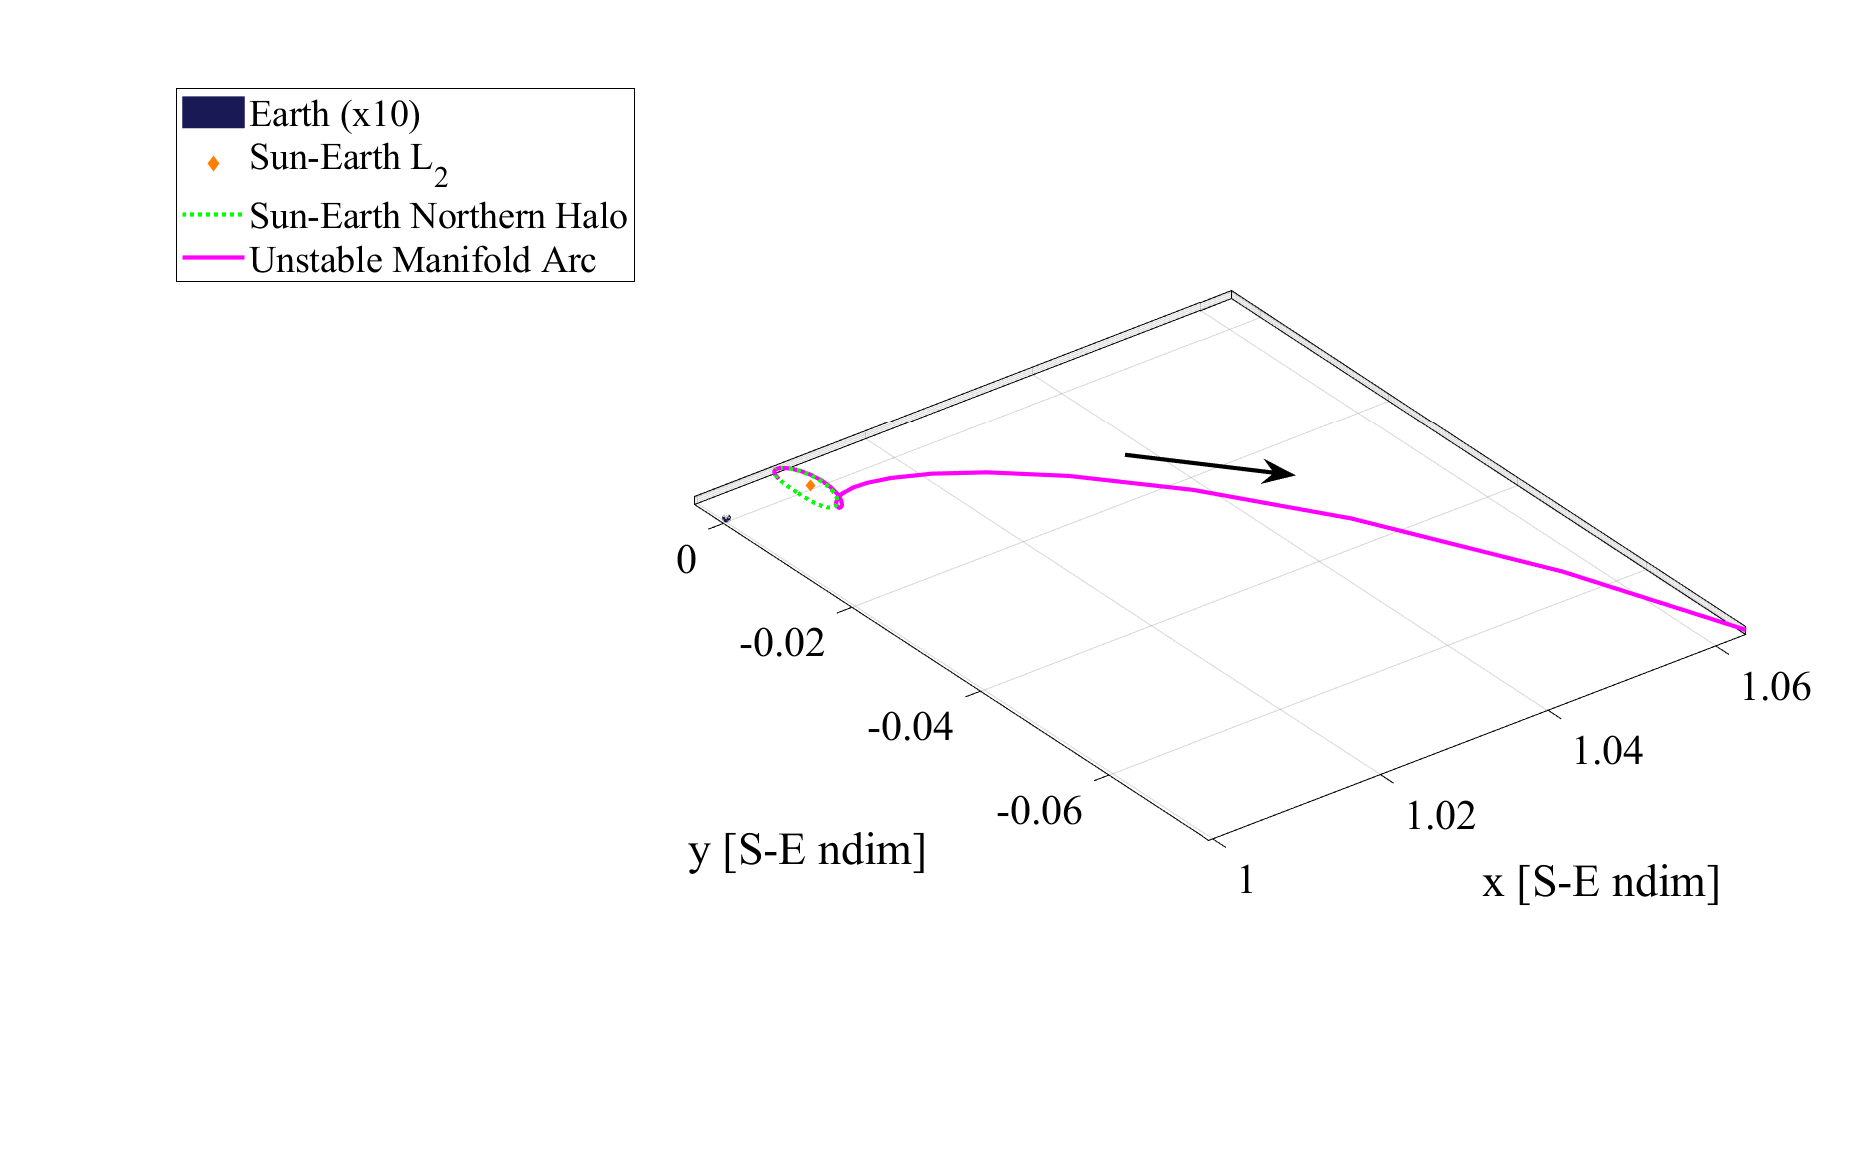
\includegraphics[width=0.9\textwidth]{figures/MinDvSE.pdf}
    \caption{MMAT departure CR3BP arc in the Sun-Earth barycentric rotating frame.}
    \label{fig:MMATSE}
\end{figure}

\begin{figure}[ht]
    \centering
    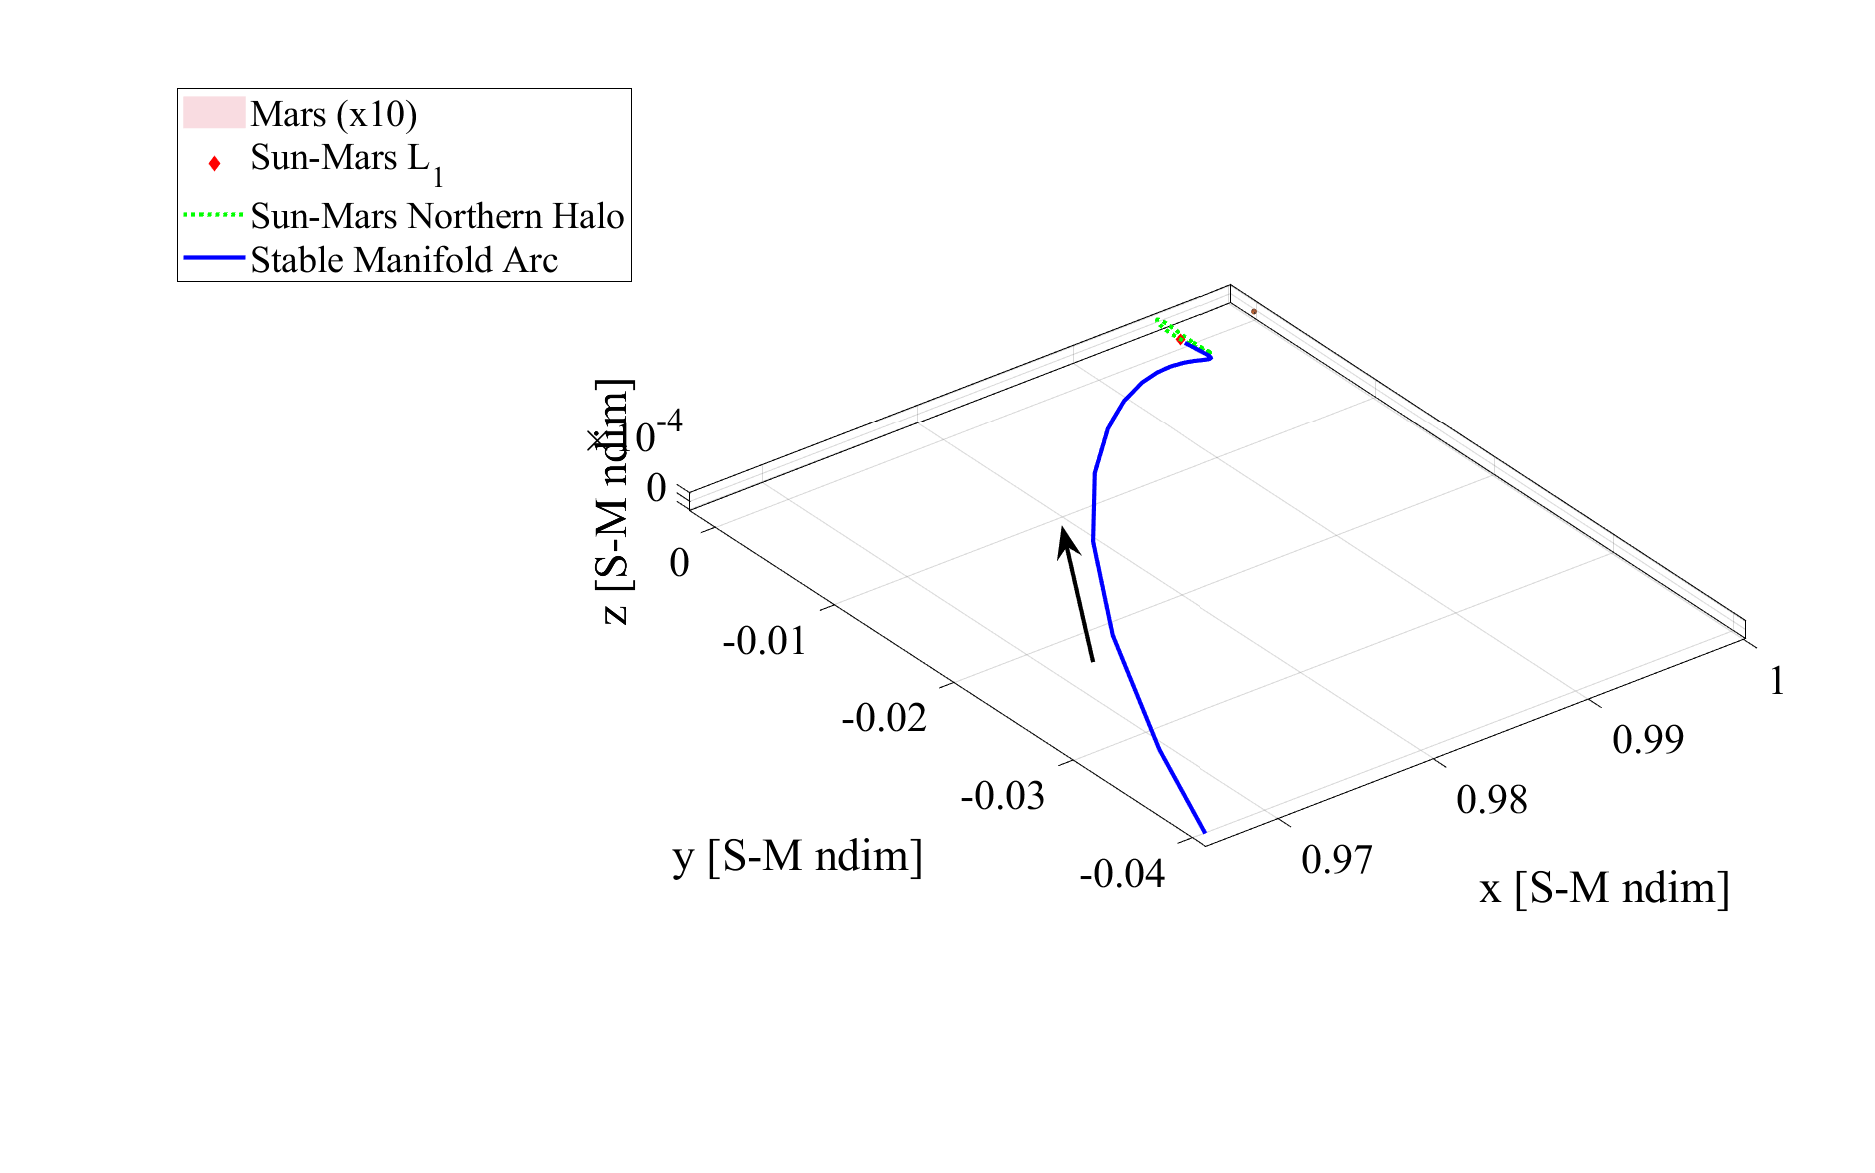
\includegraphics[width=0.9\textwidth]{figures/MinDvSM.pdf}
    \caption{MMAT arrival CR3BP arc in the Sun-Mars barycentric rotating frame.}
    \label{fig:MMATSM}
\end{figure}

In \cref{fig:MMATEvo}(a), the times-of-flight and maneuver magnitudes of the family members are
shown with respect to their initial phasing. Note that there are areas of initial epochs where
transfers could not be computed because the inequality in \cref{eq:MMAT} was not satisfied with
those orientations. Each successful epoch also has two transfer solutions corresponding to the two
arrival phasing solutions described above. The two groups of transfers in the figure correspond to 
the solutions where $n=0$ or $n=1$ satisfy \cref{eq:MMAT} and are similar due to the symmetry of
the possible bridge conic orientations for an intersection. The full time-of-flight for the
transfers is generally bounded between $3$ and $5.5$ years, while the magnitude of the two
maneuvers combined is between $4$ and $6$ km/s.

\cref{fig:MMATEvo}(b) shows the same transfers, now with the required initial Mars phasing
$\theta_{0_{Mars}}$. This plot can be used to associate each transfer with an actual launch date
where the Earth and Mars are in the specified locations in their respective orbits. Varying the
chosen manifold departure arc while keeping the initial epoch fixed creates families that would
appear as vertical lines in \cref{fig:MMATEvo}(b), providing additional launch date flexibility but
potentially at the cost of maneuver $\Delta v$.

\begin{figure}[ht]
    \begin{subfigure}[h]{0.495\linewidth}
        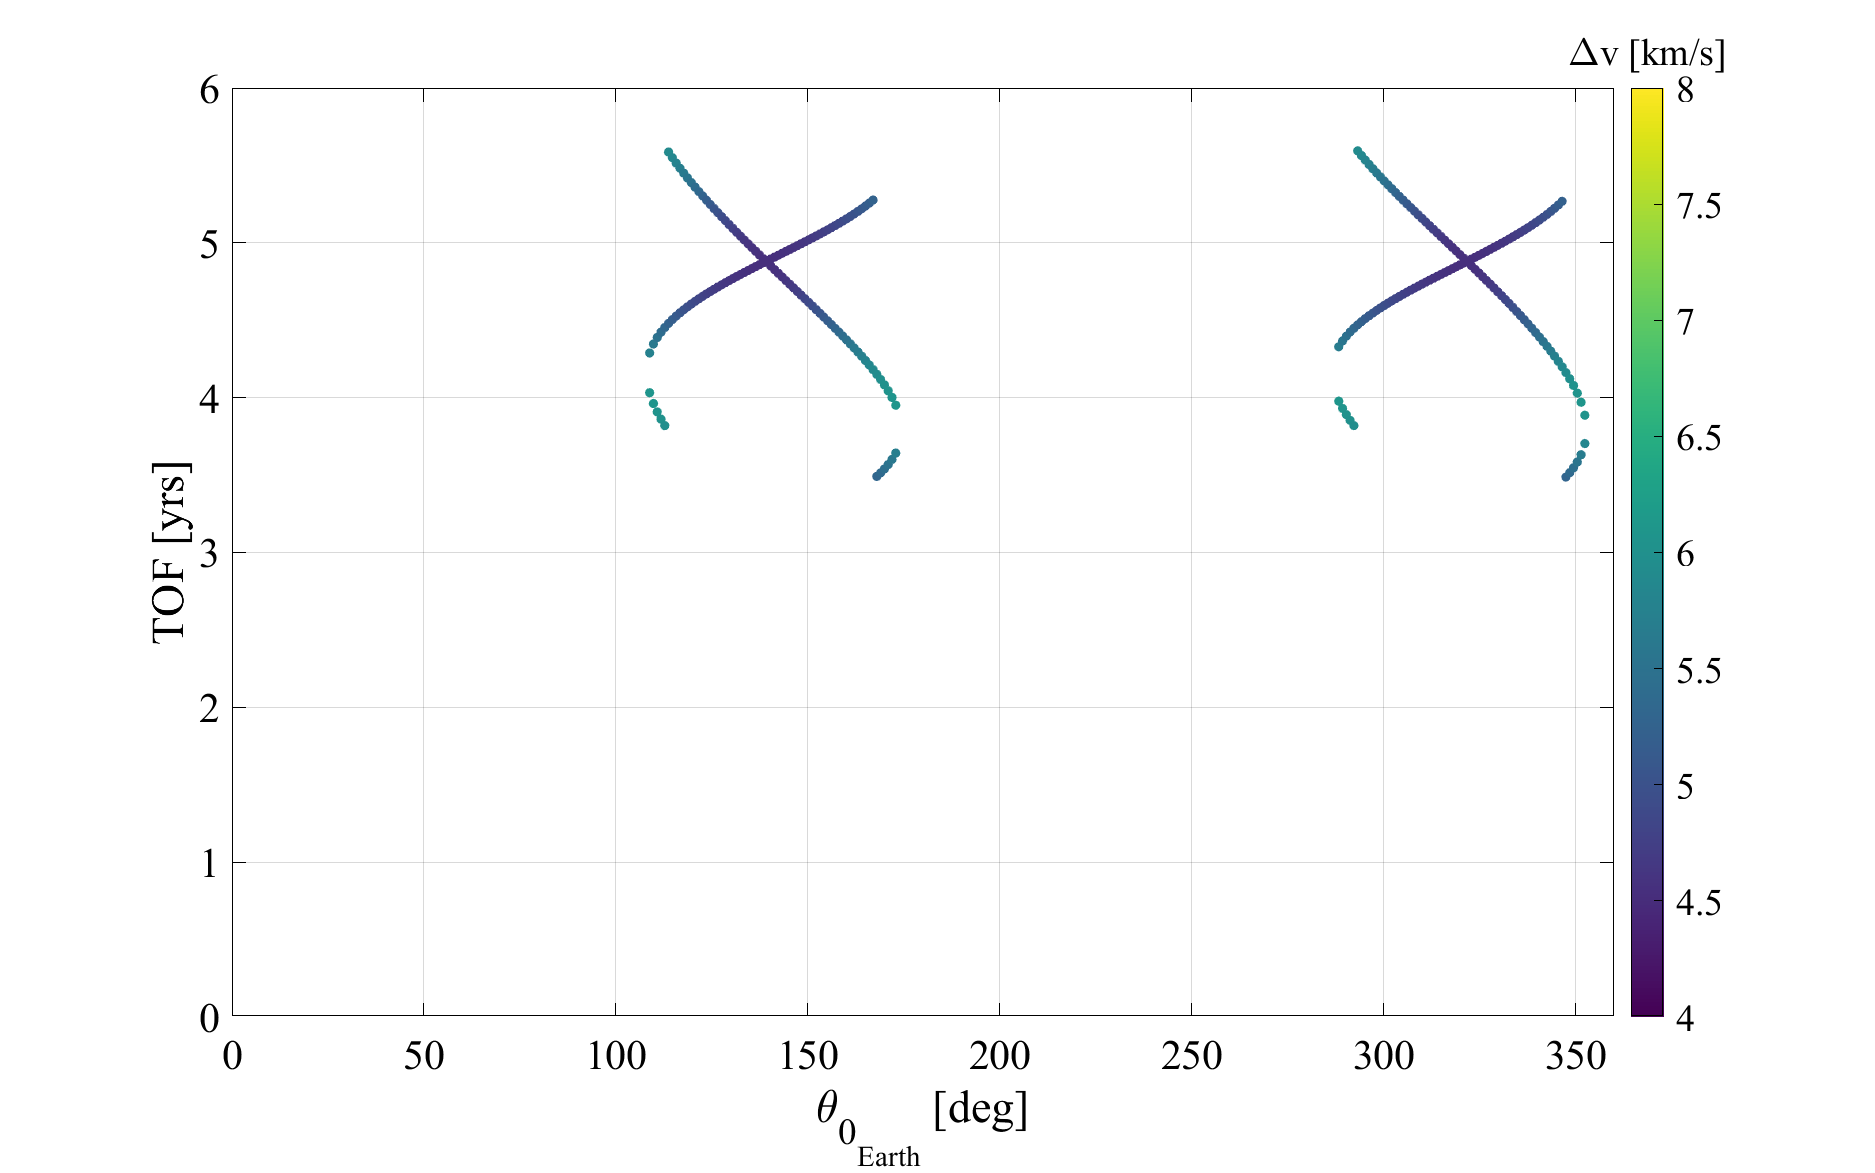
\includegraphics[width=\textwidth]{figures/MMATTOF.pdf}
        \caption{TOF and $\Delta v$}
    \end{subfigure}
    \hfill
    \begin{subfigure}[h]{0.495\linewidth}
        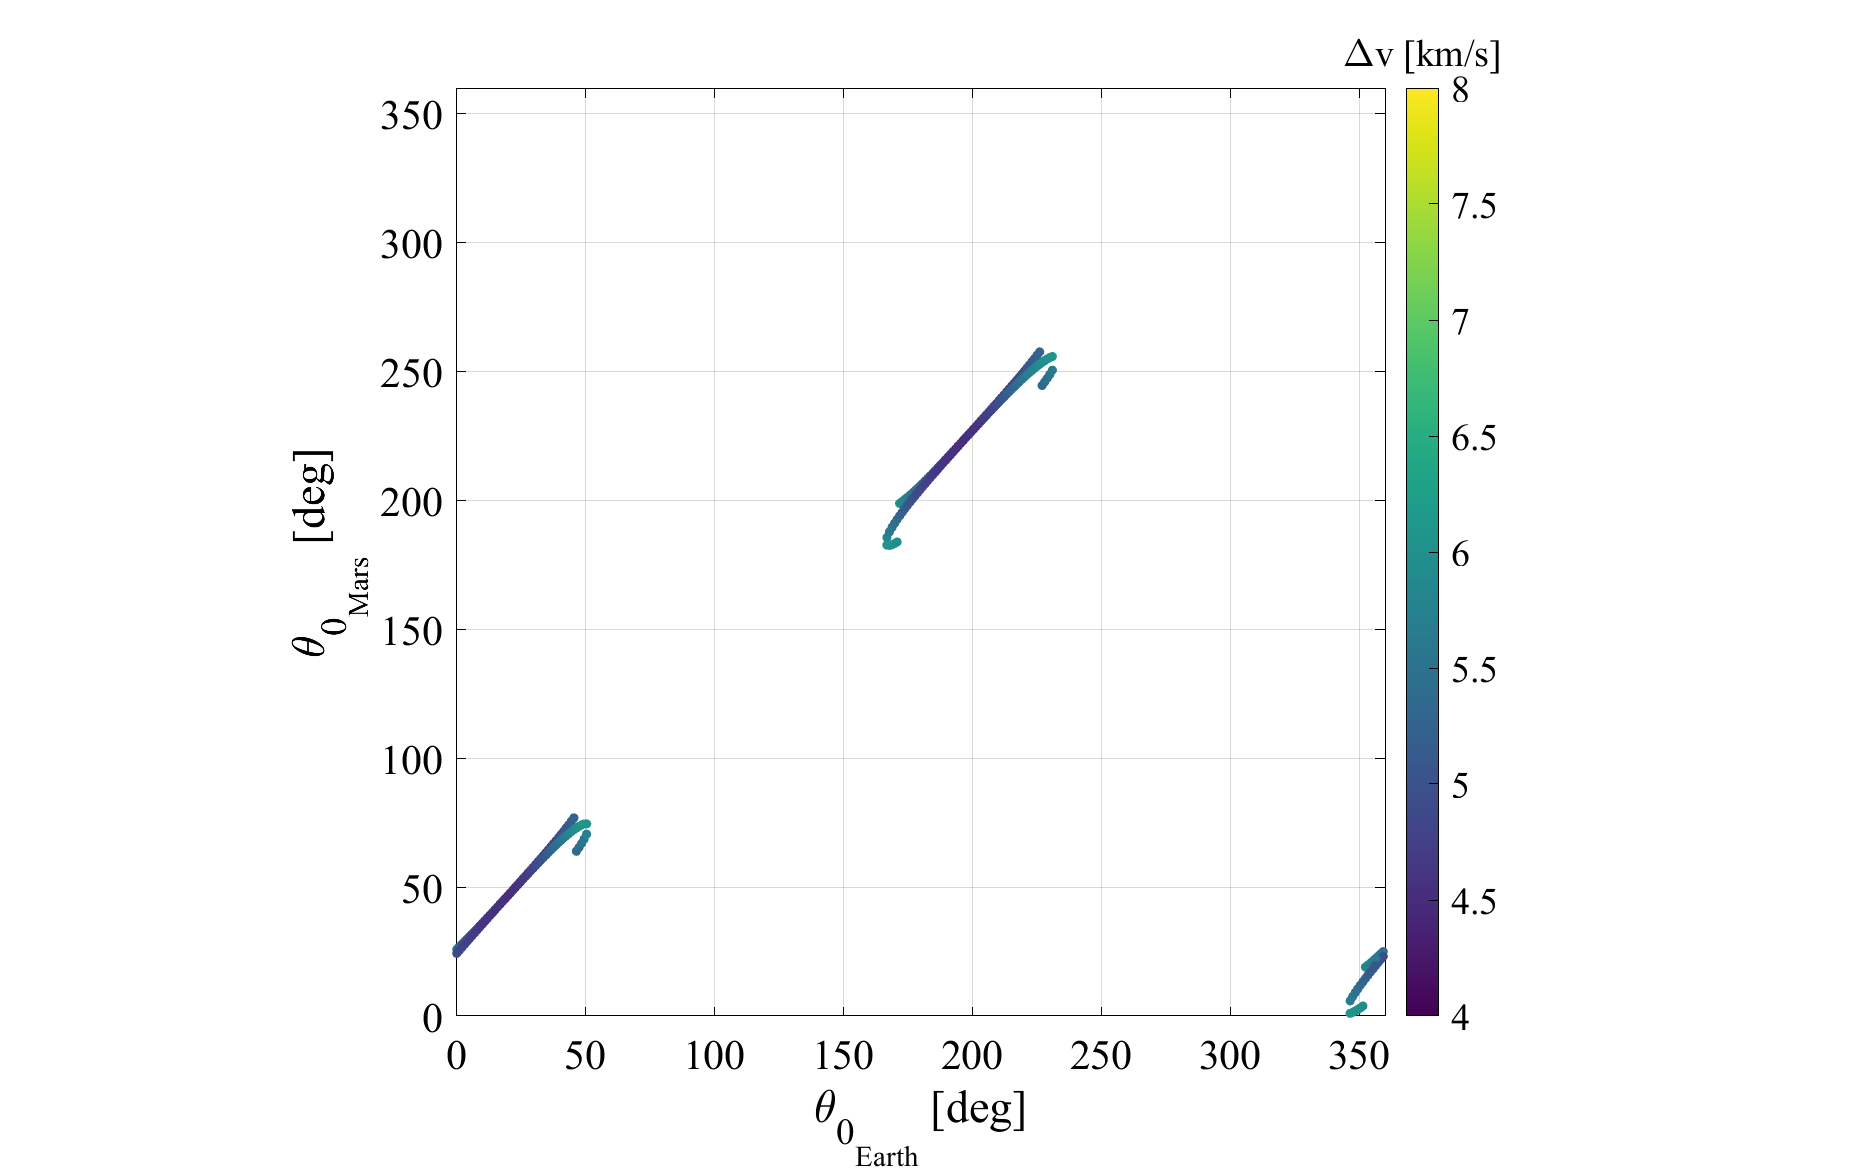
\includegraphics[width=\textwidth]{figures/MMATtheta.pdf}
        \caption{Required planet phasing}
    \end{subfigure}
    \caption{Evolution along the MMAT family continued by the initial epoch.}
    \label{fig:MMATEvo}
\end{figure}

The minimum-$\Delta v$ transfer from this family is shown in \cref{fig:MMATDv}. The total TOF of
the transfer is $1670$ days or $4.57$ years, with a total $\Delta v$ of $4.537$ km/s. In the
figure, the various arcs of the MMAT method are color-coded and the maneuvers are marked at the
beginning and end of the bridge conic arc. Note that the magenta departure CR3BP arc and the blue
arrival CR3BP arc are the same trajectories from \cref{fig:MMATSE} and \cref{fig:MMATSM}
respectively, just portrayed in the Ecliptic J2000 frame. This transfer can be compared with the
minimum-TOF transfer in \cref{fig:MMATTOF}. This transfer has a different initial epoch, which
shifts all of the arcs, and a much shorter arrival conic arc. The total TOF has decreased to $1160$
days or $3.18$ years, but the $\Delta v$ has increased to $5.298$ km/s. Note that the first
maneuver has the same magnitude; the increase comes from the second maneuver where the minimum-TOF
burn is less tangential to the bridge arc than the minimum-$\Delta v$ burn to shorten the arrival
conic arc time-of-flight. All of the other transfers in this family have similar geometries and
characteristics.

\begin{figure}[ht]
    \centering
    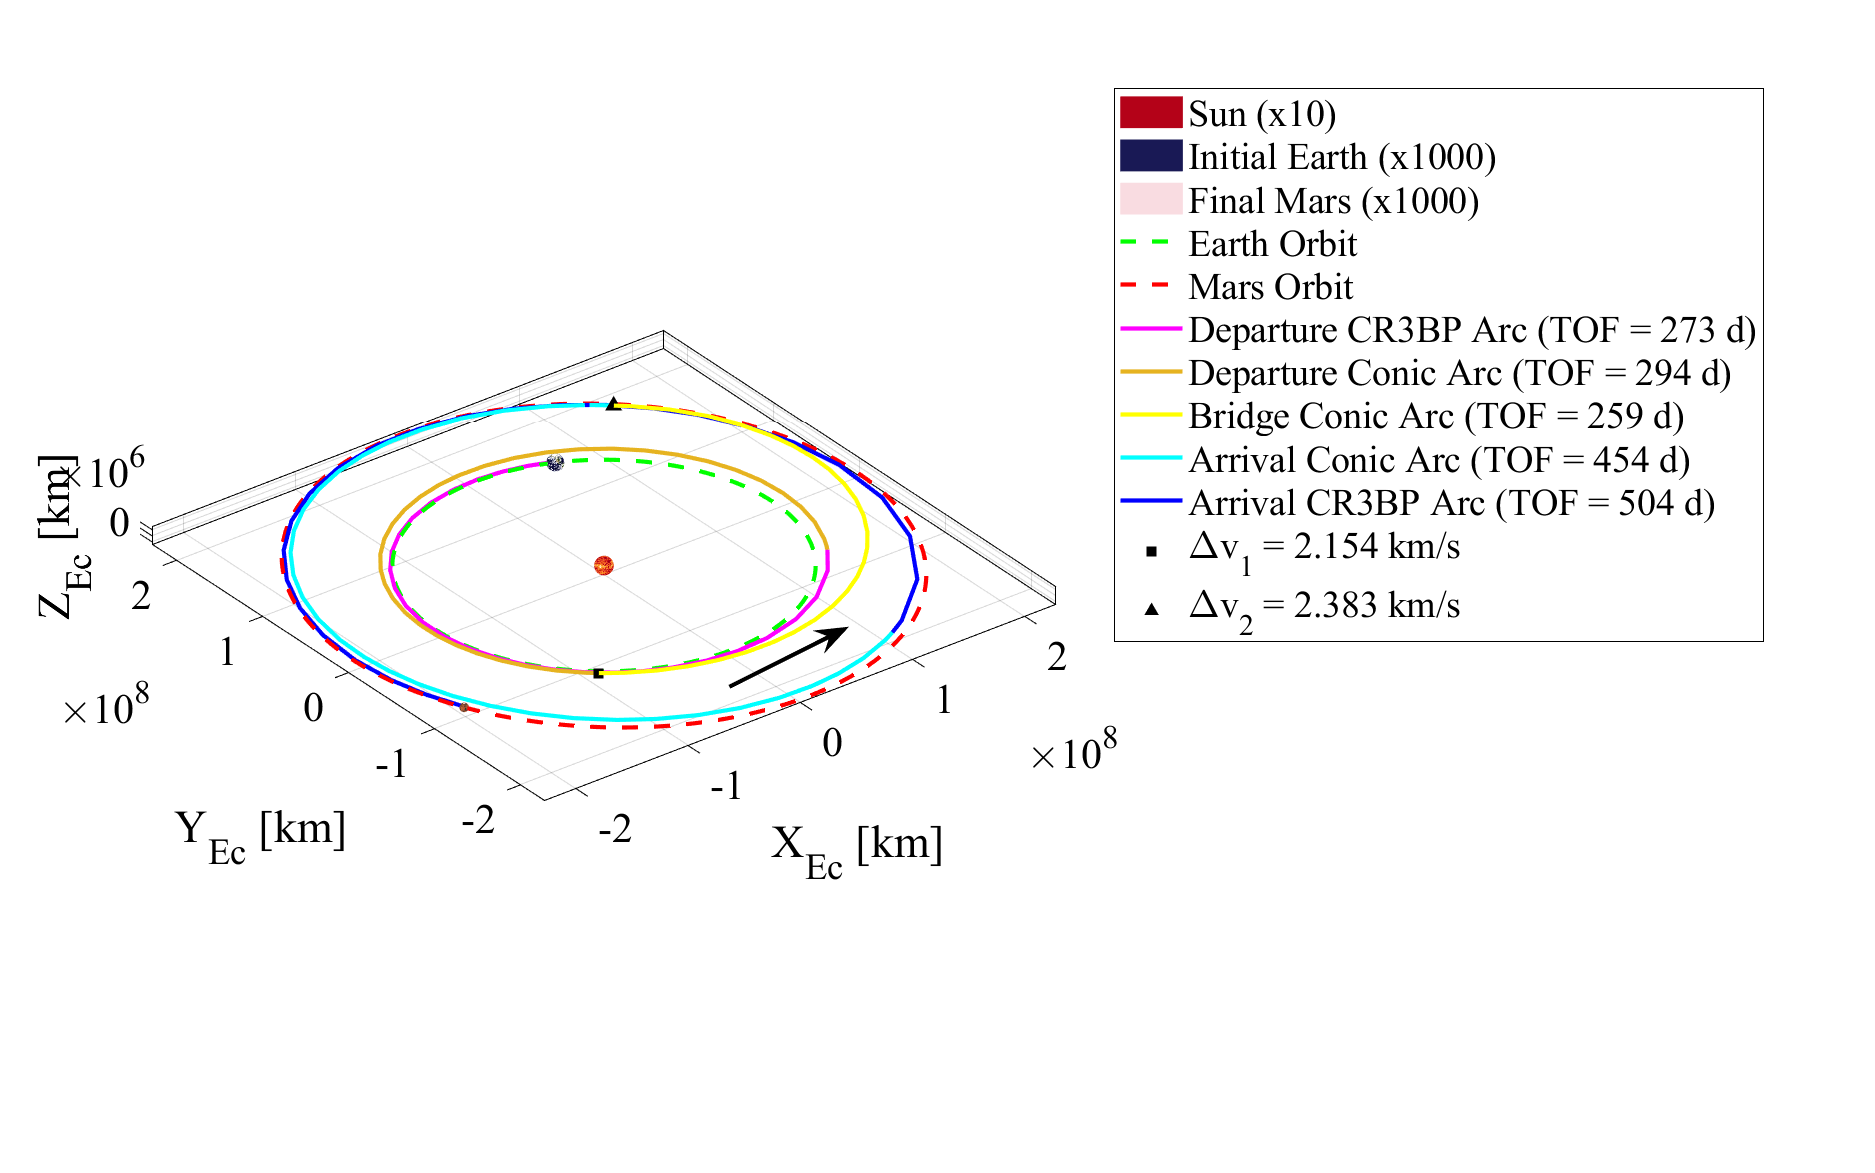
\includegraphics[width=0.9\textwidth]{figures/MinDvMMAT.pdf}
    \caption{Minimum-$\Delta v$ MMAT in the Sun-centered Ecliptic J2000 frame.}
    \label{fig:MMATDv}
\end{figure}

\begin{figure}[ht]
    \centering
    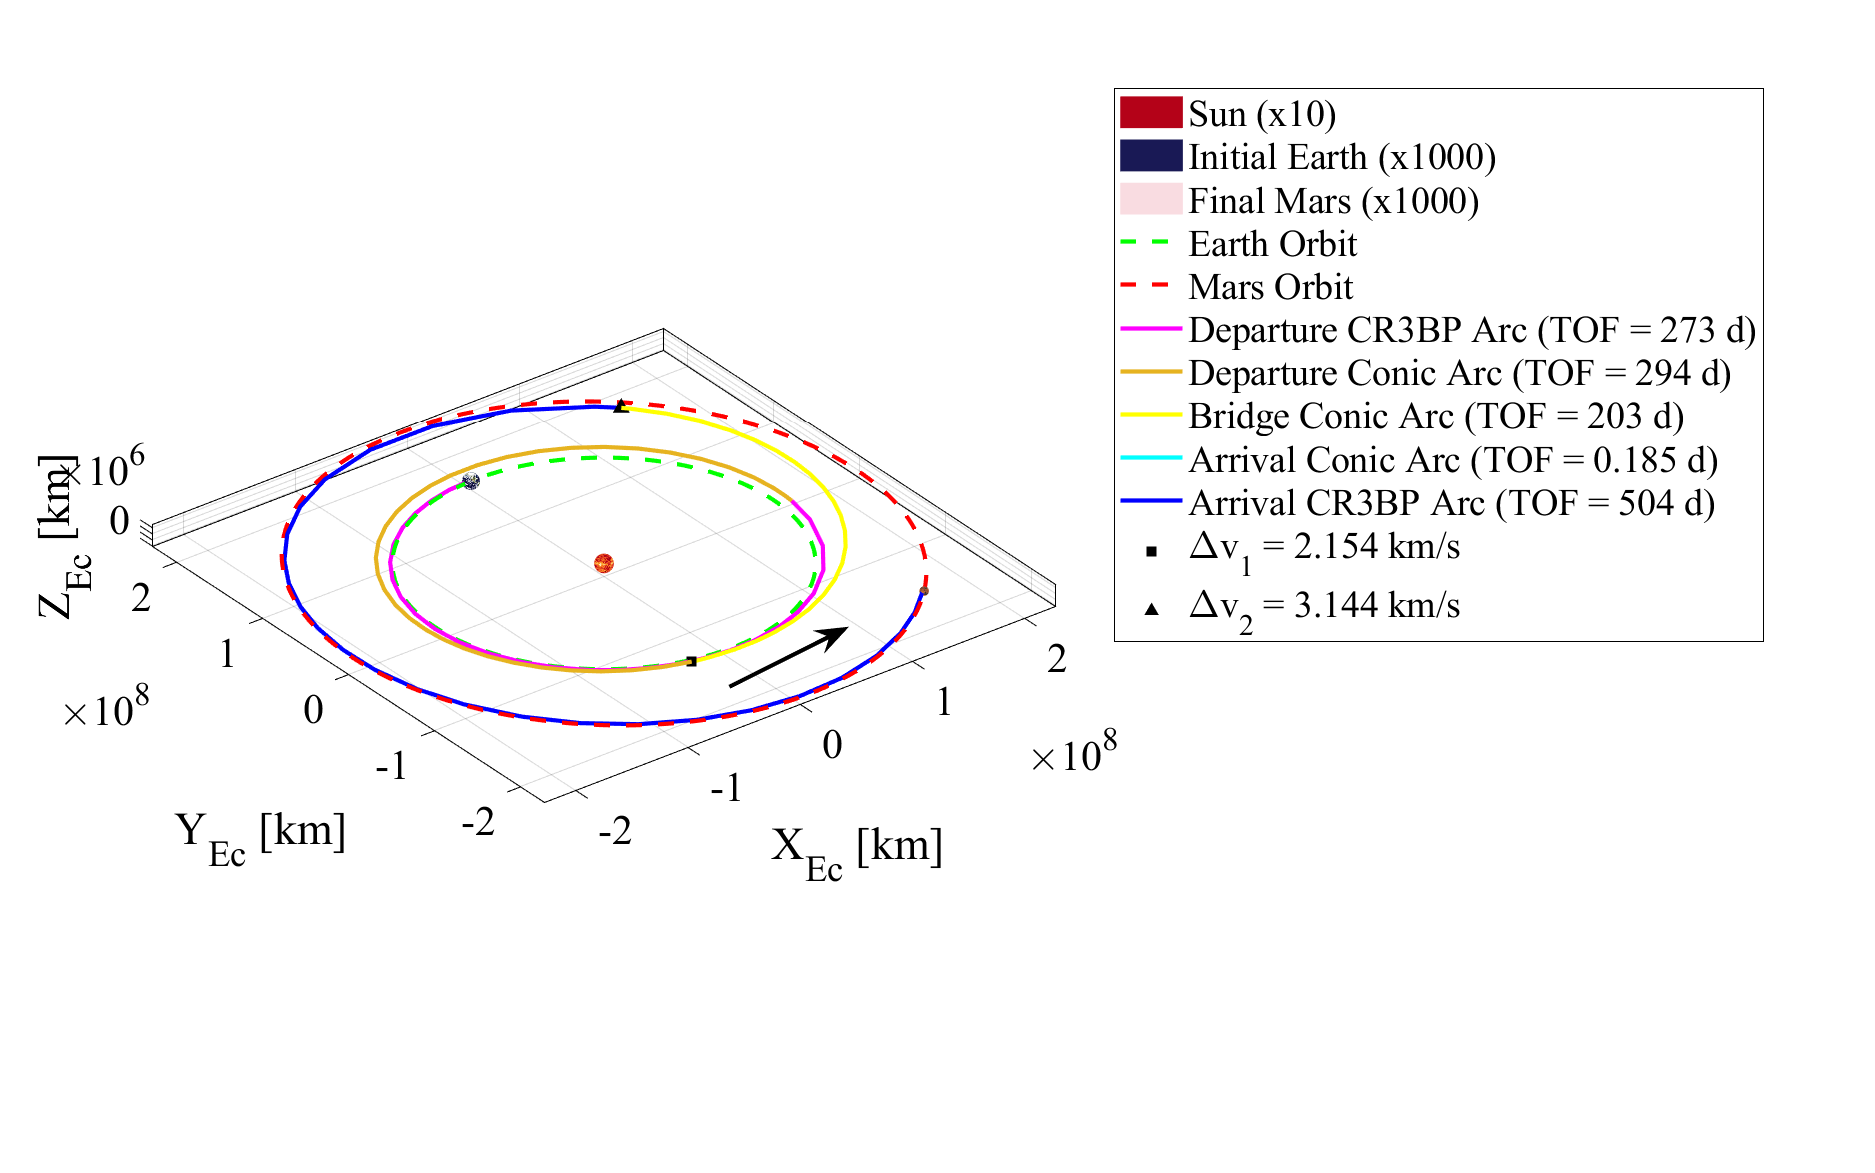
\includegraphics[width=0.9\textwidth]{figures/MinTOFMMAT.pdf}
    \caption{Minimum-TOF MMAT in the Sun-centered Ecliptic J2000 frame.}
    \label{fig:MMATTOF}
\end{figure}

\section{2BP Lambert Arcs}


\chapter{CISLUNAR DEPARTURE ORBIT COMPARISON}

\section{Transfers via Intermediate Sun-Earth Halos}

\section{Direct Transfers}

\section{Comparison to Lambert Arcs}


\chapter{CONCLUDING REMARKS}
For humanity to develop and maintain a constant presence at Mars and other deep-space locations, a
comprehensive understanding of multi-body dynamical systems theory and departure dynamics within
cislunar space is critical. This investigation develops a methodology for designing transfers from
unstable cislunar periodic orbits to deep-space targets utilizing invariant manifolds in the CR3BP.
By applying dynamical systems theory, this design approach links multiple CR3BP systems for
end-to-end transfers that exist in families of solutions, allowing for more flexible mission
designs. Additionally, in this investigation, various unstable cislunar periodic orbit families are
analyzed in the context of these interplanetary transfers to evaluate their departure
characteristics. The result is an improved understanding of invariant manifold departure behavior
in the Earth-Moon CR3BP, as well as a catalog of Mars transfer tradespaces. The end-to-end transfer
maneuver costs in this investigation are consistent with other lower-energy transfers in previous
literature and better than traditional approaches, although the time-of-flight increases
significantly. This section summarizes the contributions of this investigation and provides
several recommendations for future work.

\section{Investigation Summary}
\subsection{Low-Energy Cislunar-to-Mars Transfer Design Methodology}
Unstable periodic orbits in the CR3BP possess unstable and stable invariant manifolds that
asymptotically depart from or arrive onto the orbit and arcs from these manifolds are utilized to
construct ballistic transfers starting or terminating at these orbits. However, in the context of
interplanetary and deep-space transfers, the energy gaps between invariant manifolds of different
systems prevent direct connections between these manifolds, dictating the need for bridging arcs
or alternative strategies. The end-to-end cislunar-to-Mars transfer design methodology developed in
this investigation patches two planetary manifold arcs together with a heliocentric Keplerian
bridging arc employing the MMAT approach. Since this bridging leg of the trajectory is sufficiently
far away from both the Earth and Mars, the solar gravity is the dominating force considered and is
adequately modeled by the relative 2BP, leading to a semi-analytical method for computing this part
of the transfer. This approach is also able to incorporate the true orbital planes of Earth and
Mars, resulting in a higher model fidelity and robust framework for a transfer design to bridge
planetary systems. 

In addition to the MMAT methodology, some end-to-end transfers constructed in this investigation
stage in an intermediate $L_{2}$ halo orbit in the Sun-Earth CR3BP. Those solutions rely on
near-ballistic connections between unstable Earth-Moon and stable Sun-Earth invariant manifold arcs
for low-cost transfers in a blended CR3BP model. Solutions that instead directly depart the system
without connecting to a staging orbit still rely on this blended model, transitioning from one
CR3BP system to the other at the edge of the Moon sphere of influence. The successful meshing of
the blended CR3BP and patched 2BP-CR3BP dynamical models facilitates the end-to-end transfers
between Earth-Moon and Sun-Mars CR3BP periodic orbits.

Another major benefit of this new transfer methodology is that the transfers exist in families of
solutions. Through the exploitation of dynamical systems theory, there are a variety of ways to
continue the family of solutions. Each solution tradespace for the orbits employed in this
investigation, all of which are supplied in Appendix A, shows families of transfer solutions
continued by varying either the unstable departure manifold or the initial departure epoch. New
families could also be generated by varying the stable arrival manifold onto the Sun-Mars halo
orbit or the Jacobi constant of the intermediate staging orbit. By not relying on individual point
solutions that have to be recomputed whenever a parameter changes, the transfer methodology
developed in this investigation offers improved mission design flexibility while also providing a
broader view of the design tradespace.

\subsection{Intermediate Sun-Earth Staging Halo Orbits}
Since unstable invariant manifolds asymptotically depart from periodic orbits, the cislunar
manifold arcs take a long time to depart from the Earth-Moon system. Once they do, these manifold
arcs are propagated under the Sun-Earth dynamics until they leave the Earth SoI. In some cases, the
unstable invariant manifolds from Sun-Earth periodic orbits depart the Earth region with more
desirable characteristics. Consequently, for each cislunar departure orbit analyzed in this
investigation, transfers with direct manifold departures from the system are compared to those that
stage in an intermediate Sun-Earth $L_{2}$ northern halo orbit. This comparative analysis
identifies the optimal system departure strategy for each cislunar orbit.

In the context of the end-to-end transfer methodology developed in this investigation, it appears
that the direct departure transfers perform better overall than those that utilize a staging orbit
in terms of total maneuver $\Delta v$ cost and TOF. While staging orbit transfers for a few of the
selected orbits achieve a slightly lower average $\Delta v$, the direct transfers have lower
times-of-flight in every case analyzed. The TOF decrease can be on the order of $1$ year compared
to around $0.1$ km/s for maneuver costs. This conclusion is further reinforced by the cost function
analysis of the transfers, where all of the direct transfer families have lower cost function
values than those with staging orbits. Consequently, in this investigation, the transfers that
directly depart the Earth system appear to outperform those that stage in an intermediate Sun-Earth
halo orbit in terms of TOF and usually maneuver cost as well.

\subsection{Cislunar Departure Characteristics}
Each cislunar departure orbit included in this investigation provides families of transfer
solutions, evaluated in a tradespace between total maneuver $\Delta v$ and total TOF. For each
tradespace, a cost function is applied to determine the ten lowest-cost orbits in each family
(staging orbit and direct) based on mission design preferences. In this investigation, parameters
are selected such that decreases in TOF are valued more highly than decreases in $\Delta v$. The
characteristics of these ten lowest-cost transfers are compared between the different cislunar
departure orbits to identify characteristics across families and energy levels.

The timing and placement of the second MMAT maneuver are crucial in minimizing both the total
$\Delta v$ maneuver cost and TOF for these interplanetary transfers. For both types of transfers
developed in this investigation, the location of the second MMAT maneuver, which includes the
inclination change, is the dominating factor for the transfer total $\Delta v$ cost. The closer
this burn occurs to the periapsis of the heliocentric bridge conic arc, the lower the maneuver
cost. Additionally, in the case of transfers that directly depart the Earth vicinity, unstable
invariant manifold arcs that exit near the Sun-Earth $L_{2}$ point provide the minimum-$\Delta v$
solutions in the family. On the other hand, the main contributing factor for lowering total
transfer TOF is the relative phasing of the Keplerian conic arcs. When the true anomaly of the
arrival conic arc at the Mars SoI intersection is just after the intersection of the bridge and
arrival conic arcs, this minimizes the arrival conic arc TOF and consequently the total transfer
TOF. The minimum-TOF solutions in the families occur when the invariant manifold arcs exit near the
Sun-Earth $L_{1}$ Lagrange point; however, the lowest-cost transfers that balance the two
parameters still exit from $L_{2}$.

The selection of cislunar departure periodic orbit significantly influences both the maneuver cost
and TOF for interplanetary transfers. In terms of maneuver cost, the $L_{1}$ halo and vertical
orbit families, as well as the $L_{2}$ axial orbit family, provide the best options for staging
orbit transfers. For the transfers with direct departures, the $L_{1}$ Lyapunov and halo orbit
families result in the lowest-$\Delta v$ transfer options. The $L_{1}$ family departures leverage
close passes by the Moon to lessen the energy gap between invariant manifold arcs of two planetary
systems. When it comes to the transfer TOF, $L_{2}$ Lyapunov and halo orbit families perform the
best for staging orbit transfers, while $L_{2}$ halo, axial, and butterfly orbit families have the
fastest direct transfers. The $L_{2}$ orbit families often have invariant manifolds that depart the
Earth-Moon system faster and extend further than the $L_{1}$ orbit families. Applying the cost
function to find a balance between $\Delta v$ and TOF, this investigation identifies that transfers
from the $L_{2}$ Lyapunov, halo, and vertical orbit families with direct departures perform well at
various Jacobi constant levels. The best cislunar departure orbit identified in this investigation
is the $3.13$ $L_{2}$ Lyapunov orbit, whose lowest-cost transfers have an average maneuver cost of
$5.282$ km/s and a TOF of $3.92$ years. This analysis underscores the importance of selecting
appropriate cislunar departure orbits to achieve efficient deep-space transfers with a balance
between maneuver cost and TOF.

Employing the two interplanetary transfer methodologies developed in this investigation, all of the
included cislunar departure orbits have staging orbit and direct transfers with total maneuver
costs that are up to $1$ km/s less than the traditional Earth-Mars interplanetary transfer methods.
And while the times-of-flight of these transfers are significantly longer than traditional
interplanetary transfers due to the asymptotic nature of invariant manifolds, the transfers with
direct departures save up to $1$ year compared to the staging orbit transfers. The transfers
developed in this investigation confirm that invariant manifold arcs can be utilized to decrease
interplanetary transfer maneuver costs and highlight a few cislunar orbit families with desirable
departure characteristics.

\section{Recommendations for Future Work}
With increasing interest in interplanetary missions and the application of dynamic systems theory
in multi-body trajectory design, there are many potential avenues of future research to build off
the work done in this investigation. A few promising options are presented here:
\begin{itemize}
    \item   \textbf{Continue this analysis with cislunar departure orbits in a broader Jacobi
            constant range and transfers to other deep-space targets.}

            In the current investigation, cislunar departure orbits were limited to a Jacobi
            constant range of $2.98$-$3.13$. Many potentially useful unstable orbits and orbit
            families in the Earth-Moon CR3BP exist at Jacobi constant values outside of that range.
            For example, there are many families of resonant and period-multiplying orbits that
            were not examined in this investigation. A complete analysis of cislunar departure
            dynamics from unstable orbits would require an extension of the current analysis to
            these other orbits and families. This investigation also limited its scope by selecting
            a Sun-Mars $L_{1}$ northern halo orbit as its arrival destination. The methodologies
            developed are applicable for any unstable CR3BP arrival periodic orbit and should be
            verified with other arrival orbits and CR3BP deep-space target systems such as Venus or
            Jupiter.
    \item   \textbf{Explore cislunar departure dynamics from stable CR3BP orbits.}
    
            Unstable CR3BP departure and arrival periodic orbits are exclusively employed in this
            investigation to exploit their invariant manifolds for ballistic departures and
            arrivals. Unfortunately, the methodologies developed do not apply to stable CR3BP
            orbits due to their lack of these manifolds so other dynamical systems theory
            techniques are required. The utilization of impulsive maneuvers along the most
            stretching directions of a periodic orbit is a promising approach for stable orbit
            departure and could be applied as an alternative to invariant manifold arcs with the
            MMAT method. Muralidharan and Howell demonstrate the usefulness of such an approach
            with some applications within cislunar space\cite{Muralidharan:2022}. This approach
            opens alternative avenues for low-energy deep-space trajectory design by facilitating
            efficient departure from stable CR3BP orbits.
    \item   \textbf{Investigate strategies for incorporating dynamical systems theory and invariant
            manifolds into other interplanetary transfer design methodologies and optimization.}

            This investigation employed a combination of near-ballistic Earth-Moon to Sun-Earth
            transfers and the MMAT methodology to design interplanetary transfers, but this
            technique is not the only way to incorporate multi-body dynamical systems theory into
            deep-space trajectory design. Many other strategies exist that incorporate intentional
            Earth or Moon flybys or different maneuver counts and placements. It is possible that
            some of these methodologies could offer transfers with lower times-of-flight than those
            computed in this investigation. The transfers presented here, while they exist in
            families of solutions, are not optimized. Consequently, an exploration of other
            transfer methodologies that incorporates trajectory optimization is necessary to
            continue to improve interplanetary mission design.
    \item   \textbf{Employ other dynamical models to confirm the results of this investigation and
            further explore cislunar departure dynamics.}

            Since the gravitational effects of the Earth, Moon, and Sun are all considered at
            various stages in this investigation, depending on the dynamical model being applied,
            it would be beneficial to incorporate a 4-body model such as the BCR4BP to efficiently
            represent these dynamics. There is precedent for applying this model to the exploration
            of cislunar departure dynamics, and it would also simplify the construction of
            transfers between the Earth-Moon and Sun-Earth systems, as well as better facilitate
            the relative phasing between the celestial bodies\cite{Boudad:2021,Boudad:2022}. The
            inclusion of the solar gravitational influence in the cislunar region would also aid in
            the departure from stable cislunar orbits through pseudo-manifolds that stem from the
            inclusion of the Sun in the Earth-Moon dynamical model. Finally, the results of this
            investigation, as well as all of those proposed in this future work section, should be
            validated in a high-fidelity ephemeris force model. This validation will ensure that
            the transfer geometries persist under a more accurate representation of the dynamical
            regime while also providing insight into feasible launch dates and windows in the near
            future for these types of deep-space transfers. Transition to higher-fidelity dynamical
            models is the necessary next step for these transfers to be applied to real mission
            scenarios.
\end{itemize}


% Appendices

% Use :
%     ``\appendix''   for one appendix 
%     ``\appendices'' for more than one appendix.
\appendices

% Show list of variables if this is running in debug mode
\ifthenelse{\equal{debug}{\ZZbuildmode}} {
    \chapter*{User-Defined Variables}
\begin{center}
    \textit{Note: Currently does not support Greek letter sorting\todocomment{Would it be better ignore capitalization?}}
\end{center}


% Create database for the user-defined variables
\DTLnewdb{varDB}

% Populate database with variables, command,
%  and variables by which to srt them
\foreach \tuple in \paperVariables { 
    \DTLnewrow{varDB}
    \foreach \cmd [count=\i] in \tuple {
        \dtlexpandnewvalue
        \ifthenelse{\equal{\i}{1}}{
            \DTLnewdbentry{varDB}{Variable}{\cmd}
            \DTLnewdbentry{varDB}{VarCmd}{\expandafter\string\cmd}
        }{\DTLnewdbentry{varDB}{SortVar}{\cmd}}
    }
}
% Sort the database based on the SortVar entry
\DTLsort{SortVar}{varDB}

% Print out the sorted variables
\DTLforeach*{varDB}{\variable=Variable, \cmd=VarCmd, \sv=SortVar}{%
\noindent $\variable$: \cmd\\
}

}


%% A vita is optional for masters theses
% and required for doctoral dissertations.
% Reference: TM2017 page 13.

\begin{vita}
  [Put a brief autobiographical sketch here.]
\end{vita}
    


% Back content (vita, bib settings, etc.)
% -------------------- From Template -------------------
% Currently commented out (depends on if using BibLaTeX)

%
% This is only done if you are using BibLaTeX.
%
% \makeatletter  % commented out on 2022-01-26
%   \defbibenvironment{bibliography}
%     {%
%       \list
%         {%
%           \printtext[labelnumberwidth]%
%           {%
%             \printfield{prefixnumber}%
%             \printfield{labelnumber}%
%           }%
%         }%
%         {%
%           \setlength{\bibhang}{1in} %%%%% was 0pt
%           \setlength{\itemindent}{1in}%  -\leftmargin} %%%%% was 0pt
%           \setlength{\itemsep}{\bibitemsep}%
%           \setlength{\leftmargin}{0pt}%  .22in} % 0.42in}
%           \setlength{\parsep}{\bibparsep}%
%            \setlength{\rightmargin}{0.33in}%
%         }%
%     }
%     {\endlist}
%     {\item}
% \makeatother  % commented out on 2022-01-26



% \immediate\setlength{\labelnumberwidth}{1.5in} %%%%% was commented out
\setlength{\labelwidth}{1.5in}
\def\sllnsez{[999] }

{%
  % Make _ in URLs visible.
  % \def\t{\char'137}%
  \catcode`*=\active
  \def*{\char'137}%  \char'137 is _
  \PrintBibliography
}

\end{document}
